%\documentclass[11pt,professionalfonts,hyperref={pdftex,pdfpagemode=none,pdfstartview=FitH}]{beamer}
%\usepackage{times}
\documentclass[11pt,professionalfonts,aspectratio=169]{beamer}
\usefonttheme{serif}
\usepackage{defense_packages}
% custom macros for AAS paper


\newcommand{\linearize}[3]{\ensuremath{\left. \frac{\partial #1}{\partial #2} \right|_{#3} \delta #2}}
\newcommand{\norm}[1]{\ensuremath{\left\| #1 \right\|}}
\newcommand{\abs}[1]{\ensuremath{\left| #1 \right|}}
\newcommand{\Real}[1]{\ensuremath{\Re \left\{ #1 \right\}}}
\newcommand{\bracket}[1]{\ensuremath{\left[ #1 \right]}}
\newcommand{\braces}[1]{\ensuremath{\left\{ #1 \right\}}}
\newcommand{\parenth}[1]{\ensuremath{\left( #1 \right)}}
\newcommand{\pair}[1]{\ensuremath{\langle #1 \rangle}}
\newcommand{\met}[1]{\ensuremath{\langle\langle #1 \rangle\rangle}}
\newcommand{\refeqn}[1]{(\ref{eqn:#1})}
\newcommand{\reffig}[1]{Fig. \ref{fig:#1}}
\newcommand{\tr}[1]{\mathrm{tr}\ensuremath{\negthickspace\bracket{#1}}}
\newcommand{\trs}[1]{\mathrm{tr}\ensuremath{[#1]}}
\newcommand{\deriv}[2]{\ensuremath{\frac{\partial #1}{\partial #2}}}
\newcommand{\dderiv}[2]{\ensuremath{\frac{\partial^2 #1}{\partial^2 #2}}}
\newcommand{\dderivc}[3]{\ensuremath{\frac{\partial #1}{\partial #2 \partial #3}}}
\newcommand{\diff}[2]{\ensuremath{\frac{d #1}{d #2}}}
\newcommand{\ddiff}[2]{\ensuremath{\frac{d^2 #1}{d #2^2}}}
\newcommand{\dirDiff}[2]{\ensuremath{\mathbf{D}_{#2} #1 \cdot \delta #2}} % directional derivative
\newcommand{\SO}{\ensuremath{\mathsf{SO(3)}}}
\newcommand{\T}{\ensuremath{\mathsf{T}}}
\renewcommand{\L}{\ensuremath{\mathsf{L}}}
\newcommand{\so}{\ensuremath{\mathfrak{so}(3)}}
\newcommand{\SE}{\ensuremath{\mathsf{SE(3)}}}
\newcommand{\se}{\ensuremath{\mathfrak{se}(3)}}
\newcommand{\R}{\ensuremath{\mathbb{R}}}
\newcommand{\aSE}[2]{\ensuremath{\begin{bmatrix}#1&#2\\0&1\end{bmatrix}}}
\newcommand{\ase}[2]{\ensuremath{\begin{bmatrix}#1&#2\\0&0\end{bmatrix}}}
\newcommand{\D}{\ensuremath{\mathbf{D}}}
\newcommand{\Sph}{\ensuremath{\mathsf{S}}}
\renewcommand{\S}{\Sph}
\newcommand{\J}{\ensuremath{\mathbf{J}}}
\newcommand{\Ad}{\ensuremath{\mathrm{Ad}}}
\newcommand{\intp}{\ensuremath{\mathbf{i}}}
\newcommand{\extd}{\ensuremath{\mathbf{d}}}
\newcommand{\hor}{\ensuremath{\mathrm{hor}}}
\newcommand{\ver}{\ensuremath{\mathrm{ver}}}
\newcommand{\dyn}{\ensuremath{\mathrm{dyn}}}
\newcommand{\geo}{\ensuremath{\mathrm{geo}}}
\newcommand{\Q}{\ensuremath{\mathsf{Q}}}
\newcommand{\G}{\ensuremath{\mathsf{G}}}
\newcommand{\g}{\ensuremath{\mathfrak{g}}}
\newcommand{\Hess}[1]{\ensuremath{\mathrm{Hess} \, #1}}
\newcommand{\refprop}[1]{Proposition \ref{prop:#1}}
\newcommand{\Poincare}{Poincar\'e }
\newcommand{\vecbf}[1]{\bm{#1}}
\newcommand{\vb}[1]{\bm{#1}}
\newcommand{\vh}[1]{\hat{\bm{#1}}}
\newcommand{\slfrac}[2]{\left.#1\middle/#2\right.}

\DeclareSIUnit\px{px}

\newcommand{\vc}[1]{\ensuremath{#1}}

% relative macros
\newcommand{\rpos}{\ensuremath{x_r}}
\newcommand{\rvel}{\ensuremath{v_r}}
\newcommand{\ratt}{\ensuremath{R_r}}
\newcommand{\rdatt}{\ensuremath{\dot{R}_r}}
\newcommand{\rangvel}{\ensuremath{\Omega_r}}
\newcommand{\rhangvel}{\ensuremath{\hat{\Omega}_r}}


\usepackage[version=3]{mhchem}
\DeclareSIUnit\year{yr}
\newcommand{\hilight}[1]{\colorbox{green}{#1}}

\definecolor{mygray}{gray}{0.9}
\definecolor{RoyalBlue}{rgb}{0.25,0.41,0.88}
\def\Emph{\textcolor{RoyalBlue}}

\definecolor{tmp}{rgb}{0.804,0.941,1.0}
\setbeamercolor{numerical}{fg=black,bg=tmp}
\setbeamercolor{exact}{fg=black,bg=red}

\mode<presentation> 
{
    \usetheme[hideothersubsections,width=3.5\baselineskip]{Berkeley}
    \usefonttheme{serif}
    \setbeamercovered{transparent}
    \setbeamerfont{section in sidebar}{size=\scriptsize}
    \setbeamerfont{subsection in sidebar}{size=\tiny}
}

\makeatletter
\beamer@headheight=1.5\baselineskip

\setbeamertemplate{sidebar \beamer@sidebarside}%{sidebar theme}
  {
    \beamer@tempdim=\beamer@sidebarwidth%
    \advance\beamer@tempdim by -6pt%
    \insertverticalnavigation{\beamer@sidebarwidth}%
    \vfill
    \ifx\beamer@sidebarside\beamer@lefttext%
    \else%
      \usebeamercolor{normal text}%
      \llap{\usebeamertemplate***{navigation symbols}\hskip0.1cm}%
      \vskip2pt%
    \fi%
}%

\setbeamertemplate{footline}%{split theme}
{%
  \leavevmode%
  \begin{beamercolorbox}[wd=1\paperwidth,ht=2.5ex,dp=1.125ex,leftskip=.3cm,rightskip=.3cm]{title in head/foot}
%    \usebeamerfont{title in head/foot}\mypaper\hfill \insertframenumber/\inserttotalframenumber
    \usebeamerfont{title in head/foot}\insertshorttitle \hfill \insertframenumber/\inserttotalframenumber
  \end{beamercolorbox}
} 
\setbeamertemplate{blocks}[rounded][shadow=true]
\setbeamertemplate{title page}[default][shadow=true,rounded=true]
\setbeamercolor{box}{fg=black,bg=yellow}
\setbeamertemplate{navigation symbols}{}
\makeatother


\title[Asteroid Reconstruction]{\large\textbf Real Time Adaptive Shape Reconstruction for Asteroid Landing}

\author{\vspace*{-0.3cm}}
   
\institute{
	\footnotesize
	{\normalsize\bf{Shankar Kulumani}}\\
	\vspace*{0.2cm}
  	\textbf{Department of Mechanical \& Aerospace Engineering}\\ \vspace*{0.5cm}
 	\begin{figure} %figure%
       	
\includegraphics[width=0.75\textwidth]{gw_txh_2cs_pos}
  	\end{figure}
}
\date{20180819}

\logo{
\includegraphics[scale=0.2]{figures/gw_atx_2cs_rev.pdf}}

\begin{document}
%=======================================================%

\setcounter{framenumber}{-1}
\begin{frame} %-----------------------------%
  \titlepage
\end{frame}   %-----------------------------%

% !TEX Root = ../presentation.tex

\section{Introduction}

\subsection{Motivation}
\begin{frame}[t]{Why send spacecraft to small bodies?}
    \begin{itemize}
        \item<1-> Some properties only available at the small body
            \begin{itemize}
                \item High fidelity gravitational model
                \item Surface samples or return missions
            \end{itemize}
        \item<2-> Gain experience for future missions
            \begin{itemize}
                \item Weak gravitational field allows for less costly manuevers
                \item Asteroid tours for future deep-space human missions
            \end{itemize}
        \item<3-> Avoiding future impacts
            \begin{itemize}
                \item Local spacecraft can aid in ground based tracking
                \item Mitigation: Gravity tractors, kinetic impactors, solar sails
            \end{itemize}
    \end{itemize}

\end{frame}

\begin{frame}{Asteroid Missions}
\begin{itemize}
    \item Science - insight into the early formation of the solar system
    \item Mining - vast quantities of useful materials
    \item Impact - high risk from hazardous near-Earth asteroids
\end{itemize}    

\begin{center}
    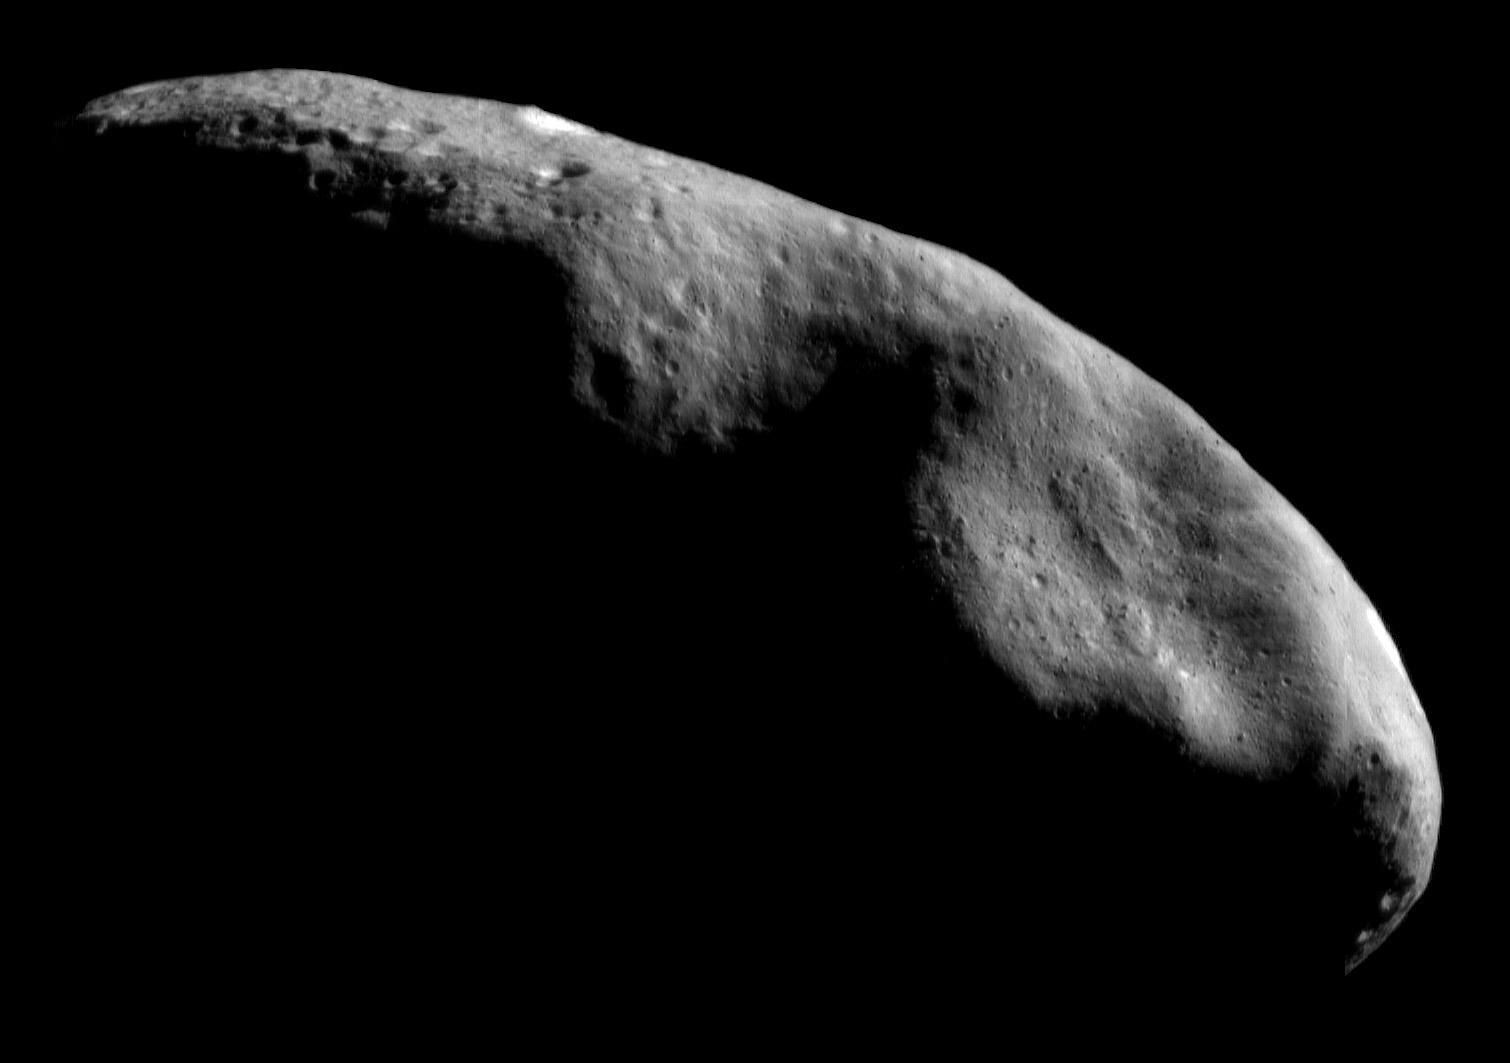
\includegraphics[height=0.5\textheight,width=0.5\textwidth,keepaspectratio]{figures/defense/near_mos_20001203_full.jpg}
    ~
    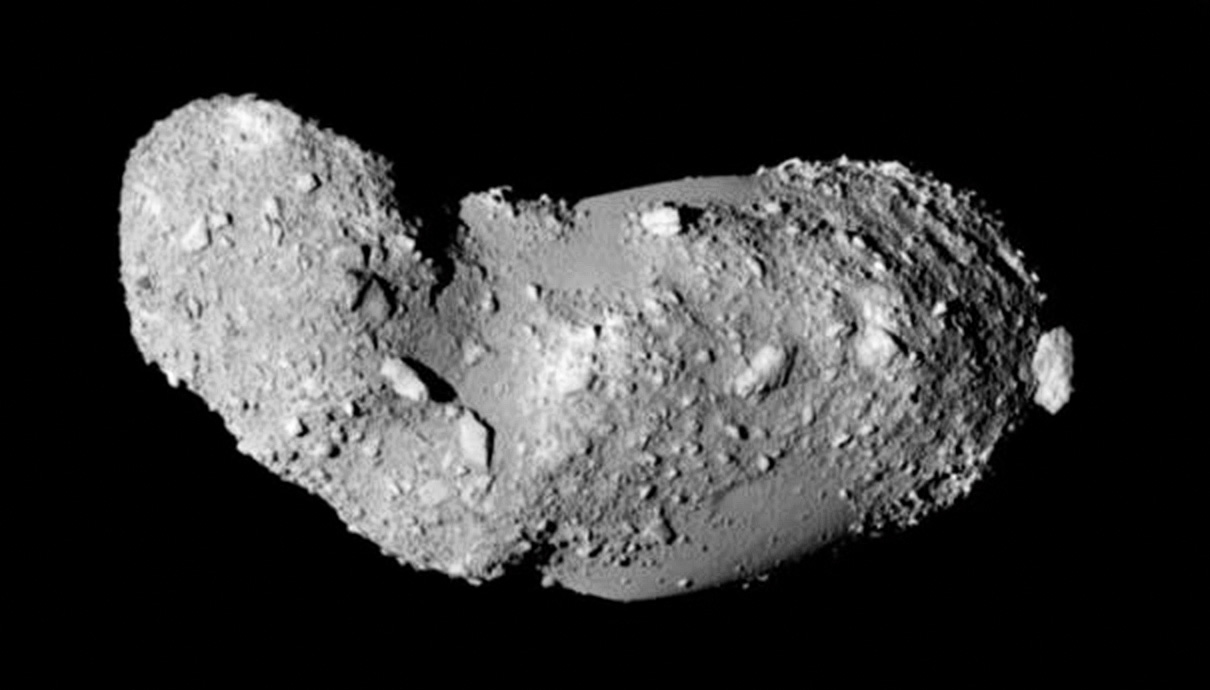
\includegraphics[height=0.5\textheight,width=0.5\textwidth,keepaspectratio]{figures/defense/Itokawa8_hayabusa_1210.jpg}
\end{center}
\end{frame}

\begin{frame}{Asteroid Mining}
    \begin{itemize}
      \item Useful materials can be extracted from asteroids to support:
      \begin{itemize}
          \item Propulsion, construction, life support, agriculture, and precious/strategic metals
      \end{itemize}
      \item Commercialization of near-Earth asteroids is feasible
    \end{itemize}

\pause

\begin{center}
\small
    \begin{tabular}{|l|r|r|}
        \hline 
        Element & Price (\SI{}{\$\per\kilo\gram}) & Sales (\SI{}{\$M\per yr}) \\
        \hline \hline 
        Phosphorous (P) & \num{0.08}  & \num{2167} \\
        Gallium (Ga) & \num{300.00}  & \num{1544} \\
        Germanium (Ge) & \num{745.00} & \num{6145} \\
        \hline \hline 
        Platinum (Pt) & \num{12394.00} & \num{1705} \\
        Gold (Au) & \num{12346.00} & \num{49} \\
        Osmium (Os) & \num{12860.00} & \num{307} \\
        \hline
    \end{tabular}
\end{center}

\end{frame}


\begin{frame}[t]{Problem statement}
    \begin{itemize}
        \item Ground based systems only provide a coarse shape estimate
        \item Spacecraft operations, e.g.\ landing, requires an accurate gravity model
        \item The gravity model accuracy is based on the accuracy of the shape
    \end{itemize}
    \pause
    \begin{center}
    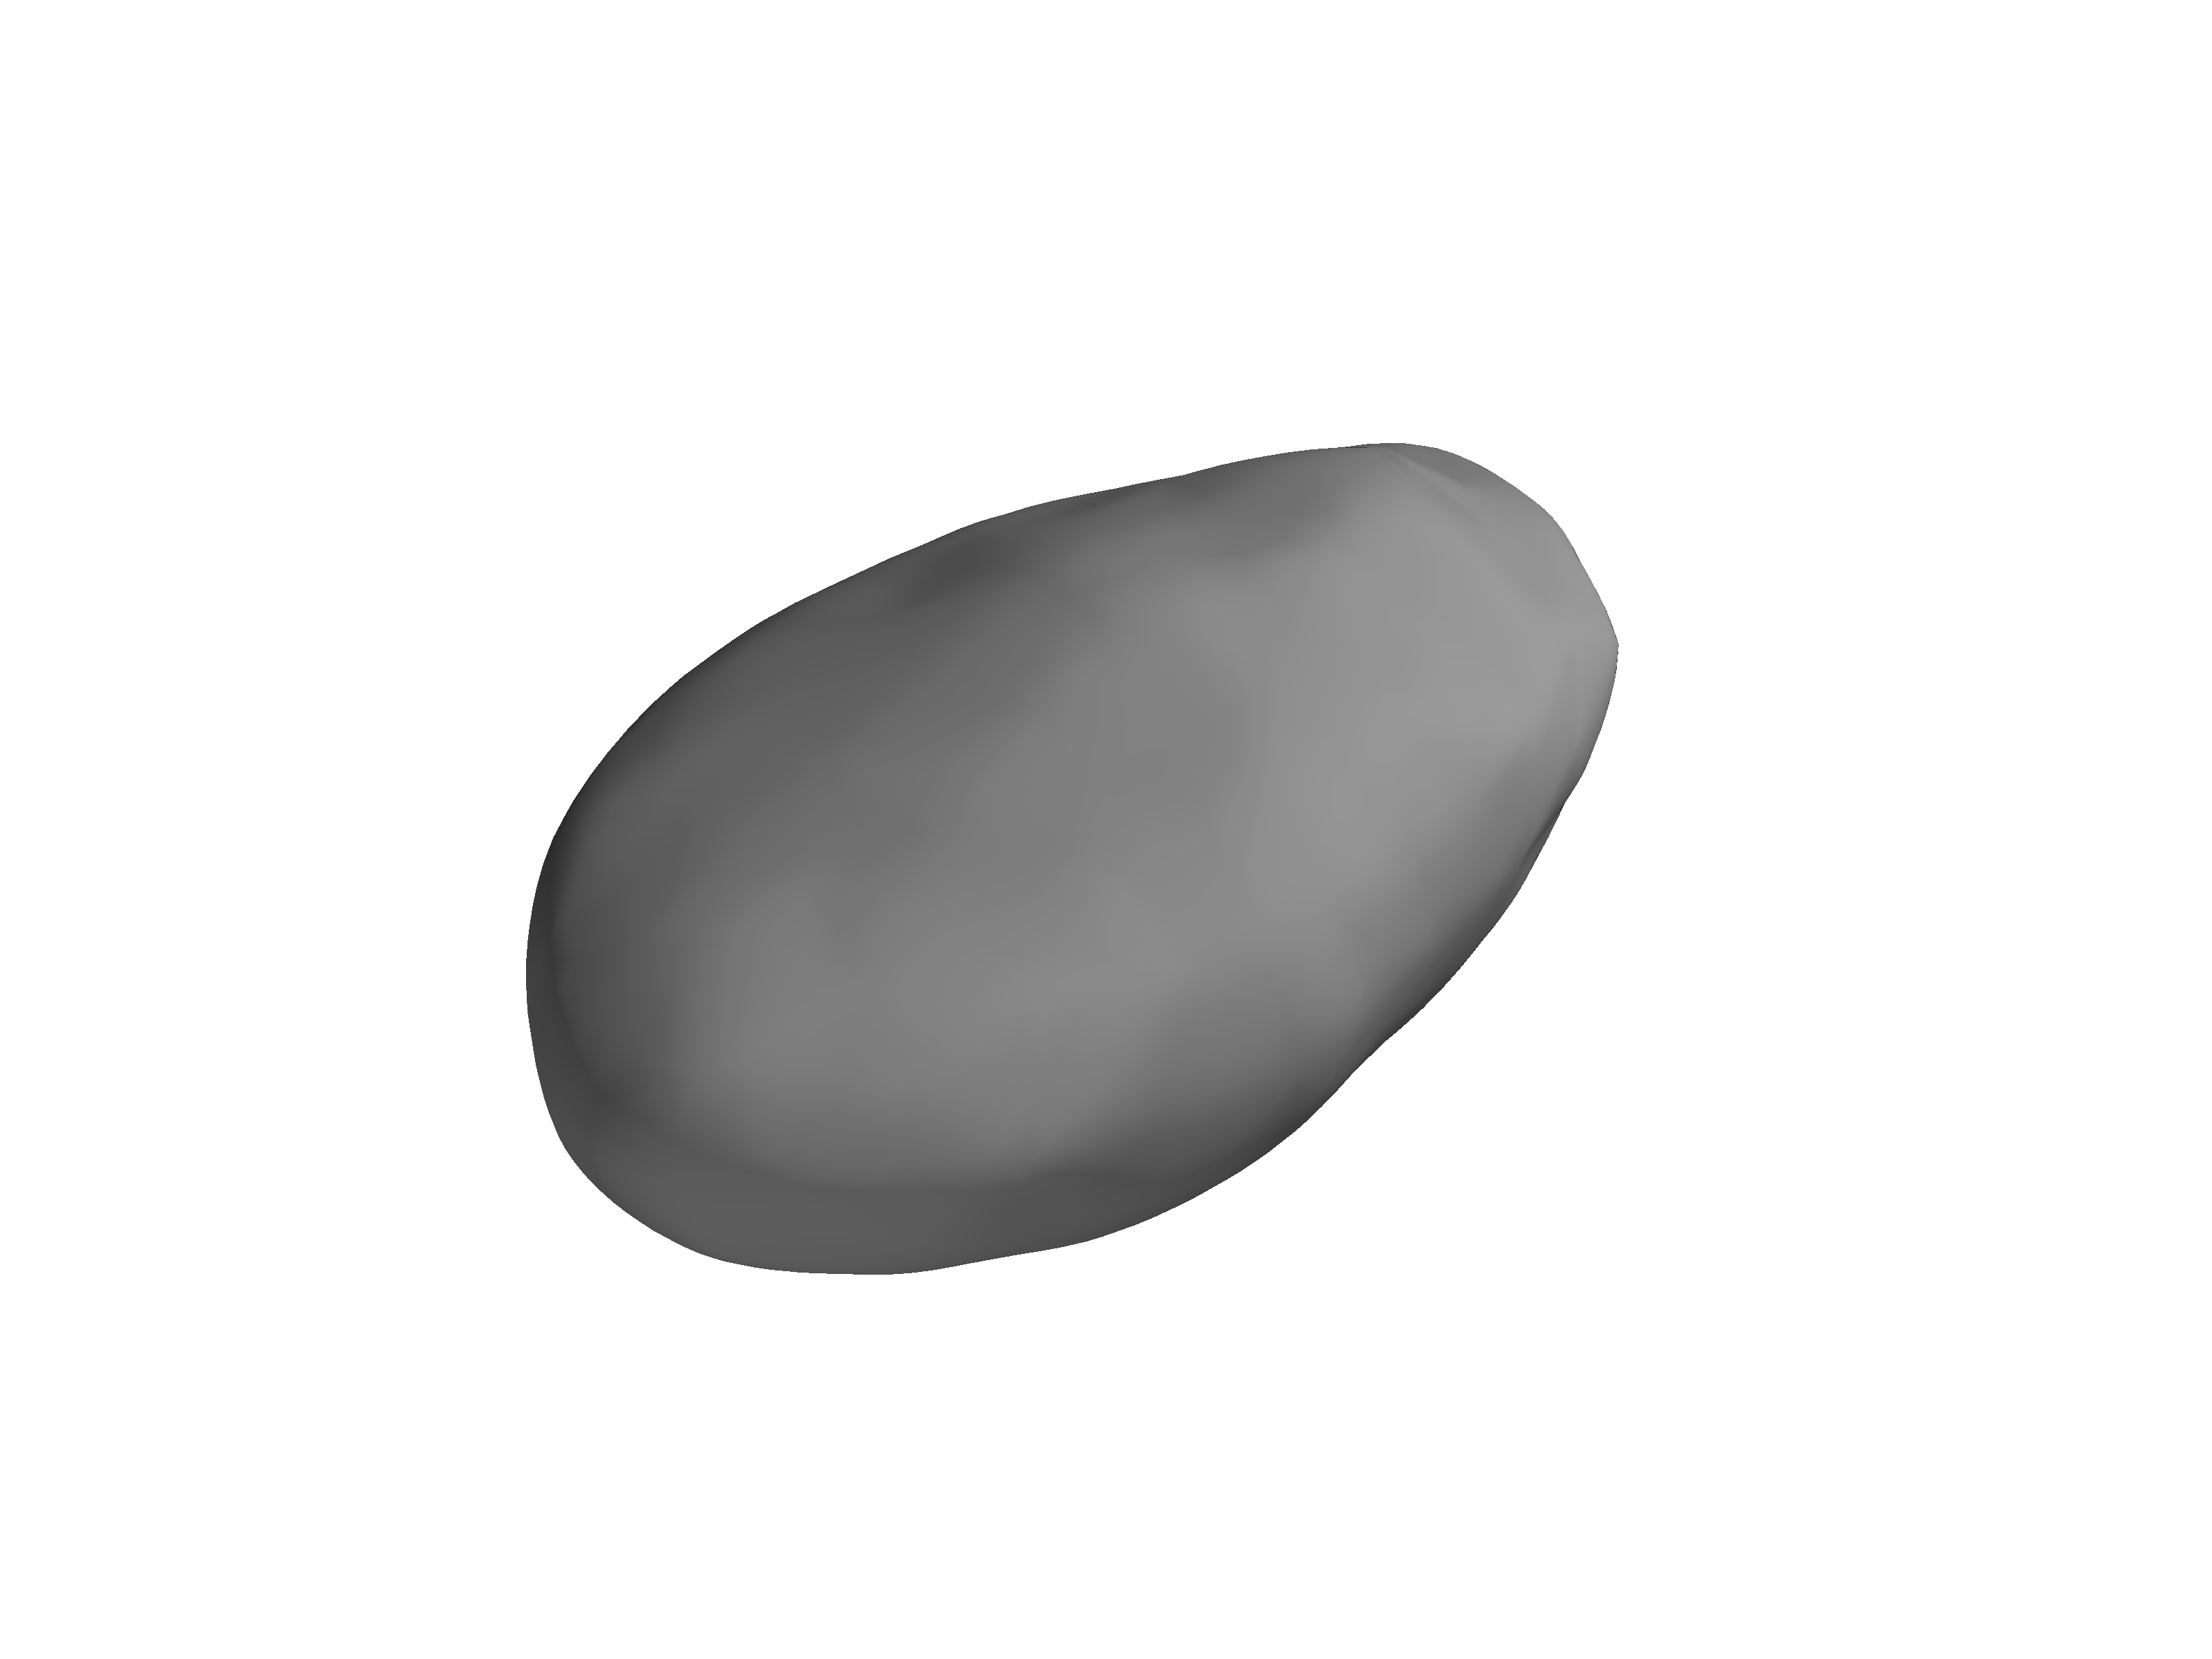
\includegraphics[trim={25cm 15cm 25cm 15cm},clip,width=0.35\textwidth,height=0.5\textheight,keepaspectratio]{figures/mathematical_background/itokawa_radar_isometric.jpg}~
    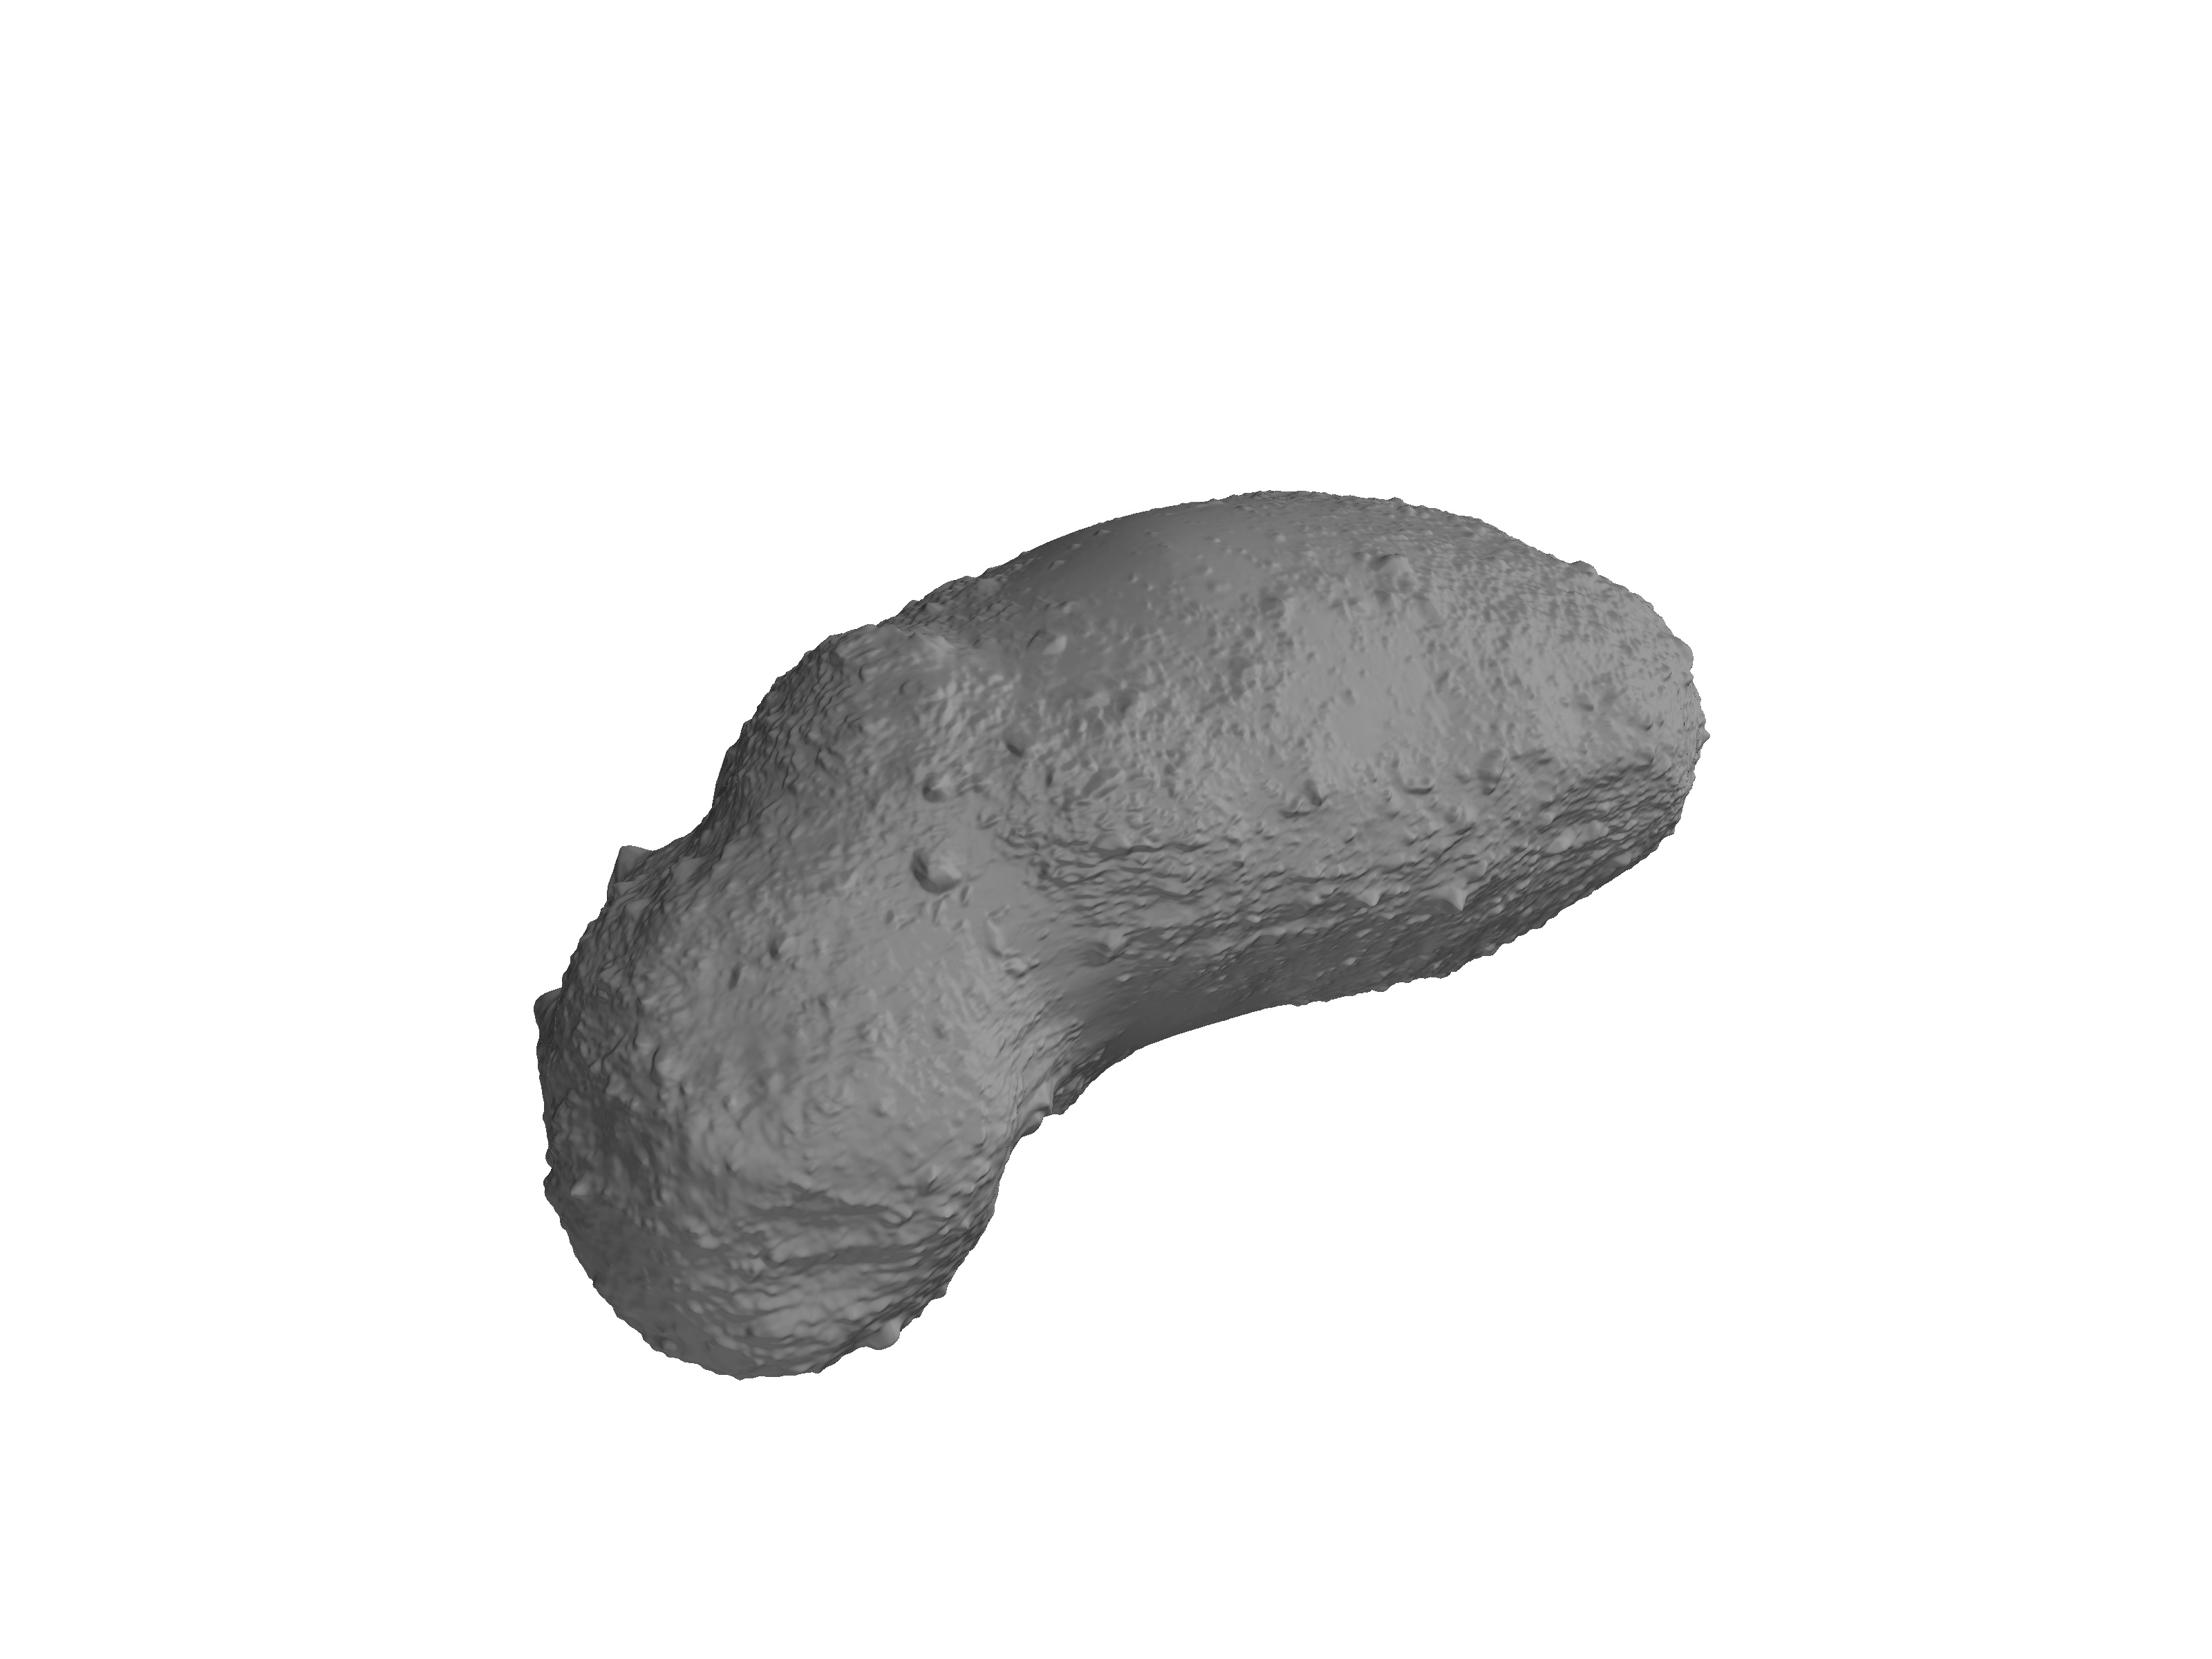
\includegraphics[trim={25cm 12cm 25cm 15cm},clip,width=0.35\textwidth,height=0.5\textheight,keepaspectratio]{figures/mathematical_background/itokawa_isometric.jpg}
    \end{center}
    \begin{block}{}
        \begin{center}
            \begin{enumerate}
                \item Need an accurate shape before arrival
                \item Only in-situ measurements can provide the required detail
            \end{enumerate}
        \end{center}
    \end{block}
    
\end{frame}





% !TEX root = ../../defense.tex

\section{System Model}

\begin{frame}{Reference Frames}

    \begin{columns}
        \begin{column}{0.5\textwidth}
            \begin{enumerate}
                \item \( \vc{e}_i \in \R^3 \) : inertial reference frame fixed in space
                \item \( \vc{f}_i \in \R^3 \) : small body fixed frame aligned with principle axes of the body
                \item \( \vc{b}_i \in \R^3 \) : spacecraft fixed frame with \( b_1 \) aligned with the symmetry axis
            \end{enumerate}
            
            \begin{block}{}
                Spacecraft state is defined on the Special Euclidean group

                \[ \parenth{R, \vc{x}} \in \SE \]
            \end{block}
        \end{column}
        \begin{column}{0.5\textwidth}
            \begin{scaletikzpicturetowidth}{2\columnwidth}
                \resizebox{\columnwidth}{!}{%
                %set the plot display orientation
%synatax: \tdplotsetdisplay{\theta_d}{\phi_d}
\tikzsetnextfilename{ref_frames}
\tdplotsetmaincoords{60}{110}
%start tikz picture, and use the tdplot_main_coords style to implement the display 
%coordinate transformation provided by 3dplot
\begin{tikzpicture}[scale=5,tdplot_main_coords]
%define polar coordinates for some vector
\pgfmathsetmacro{\rvec}{.8}
\pgfmathsetmacro{\thetavec}{30}
\pgfmathsetmacro{\phivec}{60}
\pgfmathsetmacro{\Px}{0.2}
\pgfmathsetmacro{\Py}{0.346}
\pgfmathsetmacro{\Pz}{0.693}
\pgfmathsetmacro{\b}{0.5}
\pgfmathsetmacro{\d}{0.3}

%set up some coordinates 
%-----------------------
\coordinate (O) at (0,0,0);
\coordinate (Ptikz) at (\Px, \Py, \Pz);
%determine a coordinate (P) using (r,\theta,\phi) coordinates.  This command
%also determines (Pxy), (Pxz), and (Pyz): the xy-, xz-, and yz-projections
%of the point (P).
%syntax: \tdplotsetcoord{Coordinate name without parentheses}{r}{\theta}{\phi}
% \tdplotsetcoord{P}{\rvec}{\thetavec}{\phivec}
%draw figure contents
%--------------------

%draw the main coordinate system axes
\draw[thick,-Latex] (0,0,0) -- (1,0,0) node[anchor=north east]{$e_1$};
\draw[thick,-Latex] (0,0,0) -- (0,1,0) node[anchor=north west]{$e_2$};
\draw[thick,-Latex] (0,0,0) -- (0,0,1) node[anchor=south]{$e_3 = f_3$};

%draw a vector from origin to point (P) 
\draw[-stealth,color=red, -Latex] (O) -- node [below right] {$ r $} ($(\Px, \Py, \Pz) $);

%draw the angle \phi, and label it
%syntax: \tdplotdrawarc[coordinate frame, draw options]{center point}{r}{angle}{label options}{label}
\tdplotdrawarc{(O)}{0.2}{0}{\phivec}{anchor=north}{$\Omega_A t$}


%set the rotated coordinate system so the x'-y' plane lies within the
%"theta plane" of the main coordinate system
%syntax: \tdplotsetthetaplanecoords{\phi}
\tdplotsetthetaplanecoords{\phivec}

% draw the asteroid frame
% \draw[thick,->,tdplot_rotated_coords] (0,0,0) -- (1,0,0) node[anchor=north east]{$f_3$};
\draw[thick,-Latex,tdplot_rotated_coords] (0,0,0) -- (0,1,0) node[anchor=north west]{$f_1$};
% \draw[thick,->,tdplot_rotated_coords] (0,0,0) -- (0,0,1) node[anchor=north west]{$f_2$};

%draw some dashed arcs, demonstrating direct arc drawing
\draw[dashed,tdplot_rotated_coords] (\rvec,0,0) arc (0:90:\rvec);
\draw[dashed] (\rvec,0,0) arc (0:90:\rvec);

%set the rotated coordinate definition within display using a translation
%coordinate and Euler angles in the "z(\alpha)y(\beta)z(\gamma)" euler rotation convention
%syntax: \tdplotsetrotatedcoords{\alpha}{\beta}{\gamma}
\tdplotsetrotatedcoords{\phivec}{\thetavec}{0}

%translate the rotated coordinate system
%syntax: \tdplotsetrotatedcoordsorigin{point}
\tdplotsetrotatedcoordsorigin{(Ptikz)}

%use the tdplot_rotated_coords style to work in the rotated, translated coordinate frame
\draw[thick,tdplot_rotated_coords,-Latex] (0,0,0) -- (\b,0,0) node[anchor=north west]{$b_1$};
\draw[thick,tdplot_rotated_coords,-Latex] (0,0,0) -- (0,\b,0) node[anchor=west]{$b_2$};
\draw[thick,tdplot_rotated_coords,-Latex] (0,0,0) -- (0,0,\b) node[anchor=south]{$b_3$};

% transform the first dumbbell
% rot to main
\tdplottransformrotmain{\d}{0}{0};
\tdplottransformmainscreen{\tdplotresx}{\tdplotresy}{\tdplotresz};
\pgfmathsetmacro{\DMonescreenx}{\tdplotresx};
\pgfmathsetmacro{\DMonescreeny}{\tdplotresy};

\tdplottransformrotmain{-\d}{0}{0};
\tdplottransformmainscreen{\tdplotresx}{\tdplotresy}{\tdplotresz};
\pgfmathsetmacro{\DMtwoscreenx}{\tdplotresx};
\pgfmathsetmacro{\DMtwoscreeny}{\tdplotresy};

% transform P to screen coordinates and then add
\tdplottransformmainscreen{\Px}{\Py}{\Pz};
\pgfmathsetmacro{\Pscreenx}{\tdplotresx};
\pgfmathsetmacro{\Pscreeny}{\tdplotresy};

\draw[ultra thick, color=blue, tdplot_rotated_coords] (-\d, 0, 0) -- (\d, 0, 0);

\shade[ball color=red, tdplot_screen_coords, opacity=0.3] (\Pscreenx, \Pscreeny) circle (0.03);
\shade[ball color=blue,tdplot_screen_coords] ($(\Pscreenx, \Pscreeny) + (\DMonescreenx, \DMonescreeny) + (0, 0.015)$) circle (0.03);
\shade[ball color=blue,tdplot_screen_coords] ($(\Pscreenx, \Pscreeny) + (\DMtwoscreenx, \DMtwoscreeny) + (0, -0.015)$ ) circle (0.03);

\end{tikzpicture}


            }
            \end{scaletikzpicturetowidth}
        \end{column}
    \end{columns}
\end{frame}

\begin{frame}{Spacecraft Model}
    \begin{itemize}
        \item Spacecraft modeled as a rigid dumbbell
        \item Two masses \( m_1, m_2 \in \R^1 \) connected by a rigid massless link \( l \in \R^1\)
        \item Effectively captures the mass distribution of a spacecraft
    \end{itemize}

    \resizebox{\textwidth}{!}{%
        %% helper macros

\newcommand\pgfmathsinandcos[3]{%
  \pgfmathsetmacro#1{sin(#3)}%
  \pgfmathsetmacro#2{cos(#3)}%
}
\newcommand\LongitudePlane[3][current plane]{%
  \pgfmathsinandcos\sinEl\cosEl{#2} % elevation
  \pgfmathsinandcos\sint\cost{#3} % azimuth
  \tikzset{#1/.style={cm={\cost,\sint*\sinEl,0,\cosEl,(0,0)}}}
}
\newcommand\LatitudePlane[3][current plane]{%
  \pgfmathsinandcos\sinEl\cosEl{#2} % elevation
  \pgfmathsinandcos\sint\cost{#3} % latitude
  \pgfmathsetmacro\yshift{\cosEl*\sint}
  \tikzset{#1/.style={cm={\cost,0,0,\cost*\sinEl,(0,\yshift)}}} %
}

\newcommand\DrawLongitudeCircle[4][1]{
\LongitudePlane{\angEl}{#2}
\tikzset{current plane/.prefix style={scale=#1}}
% angle of "visibility"
\pgfmathsetmacro\angVis{
atan(sin(#2)*cos(\angEl)/sin(\angEl))} %
\draw[shift={(#3, #4)}][current plane]
(\angVis:1) arc (\angVis:\angVis+180:1);
\draw[shift={(#3, #4)}][current plane,dashed]
(\angVis-180:1)arc(\angVis-180:\angVis:1);
}
\newcommand\DrawLatitudeCircle[4][1]{
\LatitudePlane{\angEl}{#2}
\tikzset{current plane/.prefix style={scale=#1}}
\pgfmathsetmacro\sinVis{
sin(#2)/cos(#2)*sin(\angEl)/cos(\angEl)}
% angle of "visibility"
\pgfmathsetmacro\angVis{
asin(min(1,max(\sinVis,-1)))}
\draw[shift={(#3, #4)}][current plane]
(\angVis:1) arc (\angVis:-\angVis-180:1);
\draw[shift={(#3, #4)}][current plane,dashed]
(180-\angVis:1)arc(180-\angVis:\angVis:1);
}

%% document-wide tikz options and styles

\tikzset{%
  >=latex, % option for nice arrows
  inner sep=0pt,%
  outer sep=2pt,%
  mark coordinate/.style={inner sep=0pt,outer sep=0pt,minimum size=3pt,
    fill=black,circle}%
}

\tikzsetnextfilename{dumbbell}
\begin{tikzpicture} % "THE GLOBE" showcase

\def\R{2} % sphere radius
\def\angEl{35} % elevation angle
\def\angAz{-105} % azimuth angle
\def\length{4} % distance from COM to M_1
\def\opacity{0.2}

% centers of the masses
\coordinate (m1) at (\length, 0);
\coordinate (m2) at (-\length, 0);

\draw [ thick, dashed, -Latex] (m2) -- ($ (m1) + (3, 0) $) node [below right] {$b_1$};
\draw [thick, dashed, -Latex] (0, 0) -- (0, \R) node [above right] {$b_2$};
% TODO Make a macro to draw a sphere at a sphefic point
\filldraw[ball color=blue, opacity=\opacity] (m1) circle (\R);
\foreach \t in {-45, 0, 45} { \DrawLatitudeCircle[\R]{\t}{\length}{0} }
\foreach \t in {-30, -60,...,-150} { \DrawLongitudeCircle[\R]{\t}{\length}{0} }

\filldraw[ball color=blue, opacity=\opacity] (m2) circle (\R);
\foreach \t in {-60,-30,...,60} { \DrawLatitudeCircle[\R]{\t}{-\length}{0} }
\foreach \t in {-5,-35,...,-175} { \DrawLongitudeCircle[\R]{\t}{-\length}{0} }

% draw from origin to center of m1
\draw[thick,-Latex] node [below right] {$\zeta$} (0, 0) --  (m1);
\draw[thick,-Latex] (m1) -- ++(30:\R) node [above right] {$\eta$};

% draw the radiaii of each mass
% \draw[thick,-Latex] (m1) -- ++(130:\R) node [above right] {$r_1$};

\end{tikzpicture}


    }
\end{frame}
\subsection{EOMs}



\begin{frame}{Equations of Motion}
    Hamilton's principle used to derive equations of motion in four forms:
    \begin{enumerate}
        \item Inertial vs. Relative 
        \item Lagrangian vs. Hamiltonian
    \end{enumerate}
    True motion of the system is a stationary point of the action integral
    \begin{align*}
        \mathcal{G} &= \int_{t_0}^{t_f} T(\dot q) - V(q) dt\\
        \pause
        \delta \mathcal{G} &= \int_{t_0}^{t_f} \delta T - \delta V dt = 0
    \end{align*}
\end{frame}

\begin{frame}{Inertial EOMs in Lagrangian Form}
    The kinetic and potential energy of the dumbbell in the inertial frame
    \begin{align*}
        T\parenth{\dot{x}, \Omega} &= \frac{1}{2} m \norm{\dot{\vc{x}}}^2 + \frac{1}{2} \tr{\vh{\Omega} J_d \vh{\Omega}^T} , \\
        V( x, R ) &=  - m_1 U \parenth{R_A^T \parenth{\vc{x} + R \vc{\rho}_1}} - m_2 U \parenth{R_A^T \parenth{\vc{x} + R \vc{\rho}_2}}. 
    \end{align*}
    \pause
    The stationary point of the action integral gives:
    \begin{align*}
        \dot{x} &= v, \\
        \parenth{m_1 + m_2} \dot{v} &= - \sum_{i=0}^2 m_i R_A \deriv{U}{z_i} + u_f, \\
        \dot{R} &= R \Omega, \\
        J \dot{\Omega} + \hat{\Omega} J \Omega &= \sum_{i=0}^2 m_i \hat{\rho}_i R^T R_A \deriv{U}{z_i} + u_m. 
    \end{align*}
\end{frame}

\subsection{Gravity}

\begin{frame}{Gravitational Models}
    \begin{center}
        \tikzsetnextfilename{newton_gravity}
\begin{tikzpicture}
    \coordinate (m1) at (0, 0);
    \coordinate (m2) at (8, 0);

    \shade[ball color=blue, opacity=0.7] (m1) circle (1.5);
    \shade[ball color=red, opacity=0.7] (m2) circle (1);

    \node[ above] at (m1) {$m_1$};
    \node[above] at (m2) {$m_2$};

    \draw[-Latex] (m1) -- ++(3, 0) node[below ] {$r$}; 
    \draw[-Latex] (m2) -- ++(-2, 0) node[above] {$F_g$};
\end{tikzpicture}

    \end{center}
    \pause
    \begin{itemize}
        \item Newton's law of gravity only applies to spherical bodies
        \item Variety of methods to represent irregular bodies
            \begin{itemize}
                \item Spherical Harmonic - not valid when close to body
                \item Constant Density Ellipsoid - only valid for ellipsoids
                \item \Emph{Polyhedron Potential} - function of shape model 
            \end{itemize}
    \end{itemize}
\end{frame}

\begin{frame}{Polyhedron Gravitation Model}

\begin{columns}
\begin{column}{0.5\textwidth}
\begin{itemize}
    \item Polyhedron: solid with flat polygonal faces
    \item Assumes a constant density
    \item Gravity depends on the shape model
\end{itemize}
\end{column}
\begin{column}{0.5\textwidth}
    \resizebox{\columnwidth}{!}{%
    \tikzsetnextfilename{polyhedron_faces}

\begin{tikzpicture}[line join=bevel,z=-5.5]
	% \draw[help lines] (-10,-10) grid (10,10); %grid
    \coordinate (A1) at (0,0,-3);
    \coordinate (A2) at (-3,0,0);
    \coordinate (A3) at (0,0,3);
    \coordinate (A4) at (3,0,0);
    \coordinate (B1) at (0,3,0);
    \coordinate (C1) at (0,-3,0);
    
    \coordinate (Acenter) at (-1, 1, 1);
    \coordinate (Bcenter) at (1, 1, 1);

    \draw (A1) -- (A2) -- (B1) -- cycle;
    \draw (A4) -- (A1) -- (B1) -- cycle;
    \draw (A1) -- (A2) -- (C1) -- cycle;
    \draw (A4) -- (A1) -- (C1) -- cycle;
    \draw [fill opacity=0.7,fill=green!80!blue] (A2) -- (A3) -- (B1) -- cycle;
    \draw [fill opacity=0.7,fill=orange!80!black] (A3) -- (A4) -- (B1) -- cycle;
    \draw [fill opacity=0.7,fill=green!30!black] (A2) -- (A3) -- (C1) -- cycle;
    \draw [fill opacity=0.7,fill=purple!70!black] (A3) -- (A4) -- (C1) -- cycle;

    \shade[ball color=blue] (A3) circle (0.1) node [below left] {$v_1$};
    \shade[ball color=blue] (B1) circle (0.1) node [above] {$v_2$};
    \shade[ball color=blue] (A2) circle (0.1) node [left] {$v_3$};

    \draw[ultra thick, -Latex] (A3) --node[right] {$h_1$}  (B1);
    \draw[ultra thick, -Latex] (B1) --node[above left] {$h_2$}  (A2);
    \draw[ultra thick, -Latex] (A2) --node[above ] {$h_3$}  (A3);
    \draw[ultra thick, -Latex] (Acenter) -- ++(-2, 2, 2) node[left] {$n_A$};
    \draw[ultra thick, -Latex] (Bcenter) -- ++(2, 2, 2) node[right] {$n_B$};
    

\end{tikzpicture}

}
\end{column}
\end{columns}
\pause
\begin{align*}
    U(\vc{r}) =& \frac{1}{2} G \sigma \sum_{e \in \text{edges}} \vc{r}_e \cdot \vc{E}_e \cdot \vc{r}_e \cdot L_e - \frac{1}{2}G \sigma \sum_{f \in \text{faces}} \vc{r}_f \cdot \vc{F}_f \cdot \vc{r}_f \cdot \omega_f 
\end{align*}
\end{frame}

% !TEX root = ../presentation.tex

\section{Shape Reconstruction}
\begin{frame}{Asteroid Shape Modeling}
    \begin{itemize}
        \item<1-> Ground radar used to compute the 3D shape of the asteroid
        \begin{itemize}
            \item Computationally intensive estimation algorithm completed on the ground 
            \item The result is still coarse and only an approximation solution
            \item Not accurate enough for low altitude or landing operations
        \end{itemize}
    \item<2-> Estimating the asteroid shape is the first step of any mission
    \begin{itemize}
        \item Months or years are devoted solely to mapping the surface
        \item Laser ranging used to accurately measure relative distance 
        \item All data is sent to the ground for processing (time and manpower intensive)
    \end{itemize}
    \end{itemize}
    
    \onslide<3->{
        \begin{block}{}
            \begin{center}
                Efficient Shape Reconstruction
            \end{center}
        \end{block}
    }
\end{frame}

\begin{frame}{Problem Statement}
\begin{enumerate}
    \item<1-> Compute the surface shape from range measurements
        \begin{itemize}
            \item Real time and incrementally build the shape
        \end{itemize}
    \item<2-> Utilize shape model in dynamics and controller
        \begin{itemize}
            \item Coupled equations of motion 
            \item Nonlinear controller for maneuvering and landing
        \end{itemize}
    \item<3-> Autonomously navigate around asteroid 
        \begin{itemize}
            \item Locate areas of poor knowledge for measurement
            \item Avoid obstacles or hazards
        \end{itemize}
\end{enumerate}
\end{frame}

\subsection{Background}

\begin{frame}{LIDAR Measurements }
    \begin{itemize}
        \item<1-> Laser pulse used to measure relative distance to surface
        \item<1-> Accurate timing gives the round trip time of flight
            \begin{align*}
                d = \frac{\Delta t}{2 c}
            \end{align*}
    \end{itemize}
    \begin{center}
        \only<1>{
            \resizebox{!}{0.6\textheight}{
                \tikzsetnextfilename{laser_range_finder}
\begin{tikzpicture}[
    block/.style={rectangle,thick,
        draw=blue!50,
        fill=blue!20, 
        rounded corners, 
        text centered, 
        minimum height = 3em, 
        minimum width=6em},
        on grid=false,
        node distance=3em,
        auto,
    ]

    \node [block, blur shadow] (detector) {Detector};
    \node [block, below = of detector, blur shadow] (amplifier) {Amplifier};
    \node [block, right = of amplifier, blur shadow] (transmitter) {Transmitter};
    \node [block, below = of $(amplifier)!0.5!(transmitter)$, blur shadow] (timer)  {Clock};
    \node [block, right = of detector, blur shadow] (beamsplitter) {Optics};
    \node [block, right = of beamsplitter, blur shadow] (target) {Target};
    
    \node [below = of timer] (system) {};

    \draw[-Latex] (amplifier) |- node[left] {\scriptsize Stop pulse}  (timer.west);
    \draw[-Latex] (transmitter.south) |- node[right] {\scriptsize Start pulse} (timer.east);
    \draw[-Latex] (detector.south) -- (amplifier.north);

    \draw[-Latex] (transmitter.north) -- (beamsplitter.south);
    \draw[->,decorate,
        decoration={snake,amplitude=.4mm,segment length=2mm,post length=1mm}] (beamsplitter.350) -- (target.190);
    \draw[->,decorate,
        decoration={snake,amplitude=.4mm,segment length=2mm,post length=1mm}] (target.170) -- (beamsplitter.10);

    \draw[-Latex] (beamsplitter) -- (detector);
    \draw[-Latex] (timer) -- node[left] {\scriptsize $\Delta t$} (system);
\end{tikzpicture}

            }
        }
        \only<2>{
            \tikzsetnextfilename{frustrum}
\begin{tikzpicture}[scale=1.7]

    \pgfmathsetmacro{\posalongpath}{0.37}
    \pgfmathsetmacro{\distance}{6};
    \pgfmathsetmacro{\nearplane}{0.37};
    \pgfmathsetmacro{\hfov}{15};
    \pgfmathsetmacro{\wfov}{15};
    \pgfmathsetmacro{\H}{\distance*tan(\hfov/2)};
    \pgfmathsetmacro{\W}{\distance*tan(\wfov/2)};
    \pgfmathsetmacro{\dlength}{1};

    \pgfmathsetmacro{\conex}{1};
    \pgfmathsetmacro{\coney}{0};
    \pgfmathsetmacro{\conez}{0};

    \pgfmathsetmacro{\ctwox}{0};
    \pgfmathsetmacro{\ctwoy}{1};
    \pgfmathsetmacro{\ctwoz}{0};

    \pgfmathsetmacro{\cthreex}{0};
    \pgfmathsetmacro{\cthreey}{0};
    \pgfmathsetmacro{\cthreez}{1};
    
    \coordinate (V) at (0,0,0);
    \coordinate (A) at ($ (\distance * \conex, \distance * \coney, \distance * \conez) + (-\W * \ctwox, -\W * \ctwoy, -\W * \ctwoz) + ( \H * \cthreex, \H * \cthreey, \H * \cthreez) $);
    \coordinate (B) at ($ (\distance * \conex, \distance * \coney, \distance * \conez) + (\W * \ctwox, \W * \ctwoy, \W * \ctwoz) + ( \H * \cthreex, \H * \cthreey, \H * \cthreez) $);
    \coordinate (C) at ($ (\distance * \conex, \distance * \coney, \distance * \conez) + (\W * \ctwox, \W * \ctwoy, \W * \ctwoz) + ( -\H * \cthreex, -\H * \cthreey, -\H * \cthreez) $);
    \coordinate (D) at ($ (\distance * \conex, \distance * \coney, \distance * \conez) + (-\W * \ctwox, -\W * \ctwoy, -\W * \ctwoz) + ( -\H * \cthreex, -\H * \cthreey, -\H * \cthreez) $);

    \coordinate (m1) at ($ (V) + (\dlength * \conex, \dlength * \coney, \dlength * \ctwoz )$);
    \coordinate (m2) at ($ (V) - (\dlength * \conex, \dlength * \coney, \dlength * \ctwoz )$);

    \path (A) -- (V) coordinate[pos=\posalongpath] (A-V);
    \path (B) -- (V) coordinate[pos=\posalongpath] (B-V);
    \path (C) -- (V) coordinate[pos=\posalongpath] (C-V);
    \path (D) -- (V) coordinate[pos=\posalongpath] (D-V);
    
    % labels of points
    \node[below] at (A) {$A$};
    \node[above] at (B) {$B$};
    \node[above] at (C) {$C$};
    \node[right] at (D) {$D$};
    
    \shade[ball color=red] (A) circle (0.05);
    \shade[ball color=red] (B) circle (0.05);
    \shade[ball color=red] (C) circle (0.05);
    \shade[ball color=red] (D) circle (0.05);

    \draw[red!50!black, dashed] (V) -- (A-V) (V) -- (B-V) (V) -- (C-V) (V) -- (D-V);
    % \draw[red!50!black] (A) -- (A-V) (B) -- (B-V) (C) -- (C-V) (D) -- (D-V);
    \draw[red!50!black, -Latex] (A-V) -- (A);
    \draw[red!50!black, -Latex] (B-V) -- (B);
    \draw[red!50!black, -Latex] (C-V) -- (C);
    \draw[red!50!black, -Latex] (D-V) -- (D);
    \fill[red,opacity=0.5,draw=red!80!black,thick] (A) -- (B) -- (C) -- (D) -- cycle;
    \fill[blue,opacity=0.5,draw=blue!80!black,thick] (A-V) -- (B-V) -- (C-V) -- (D-V) -- cycle; 
    
    \draw[blue!50!black, ultra thick] (m1) -- (m2);
    \shade[ball color=blue] (m1) circle (0.2);
    \shade[ball color=blue] (m2) circle (0.2);

\end{tikzpicture}

        }
        \only<3>{
            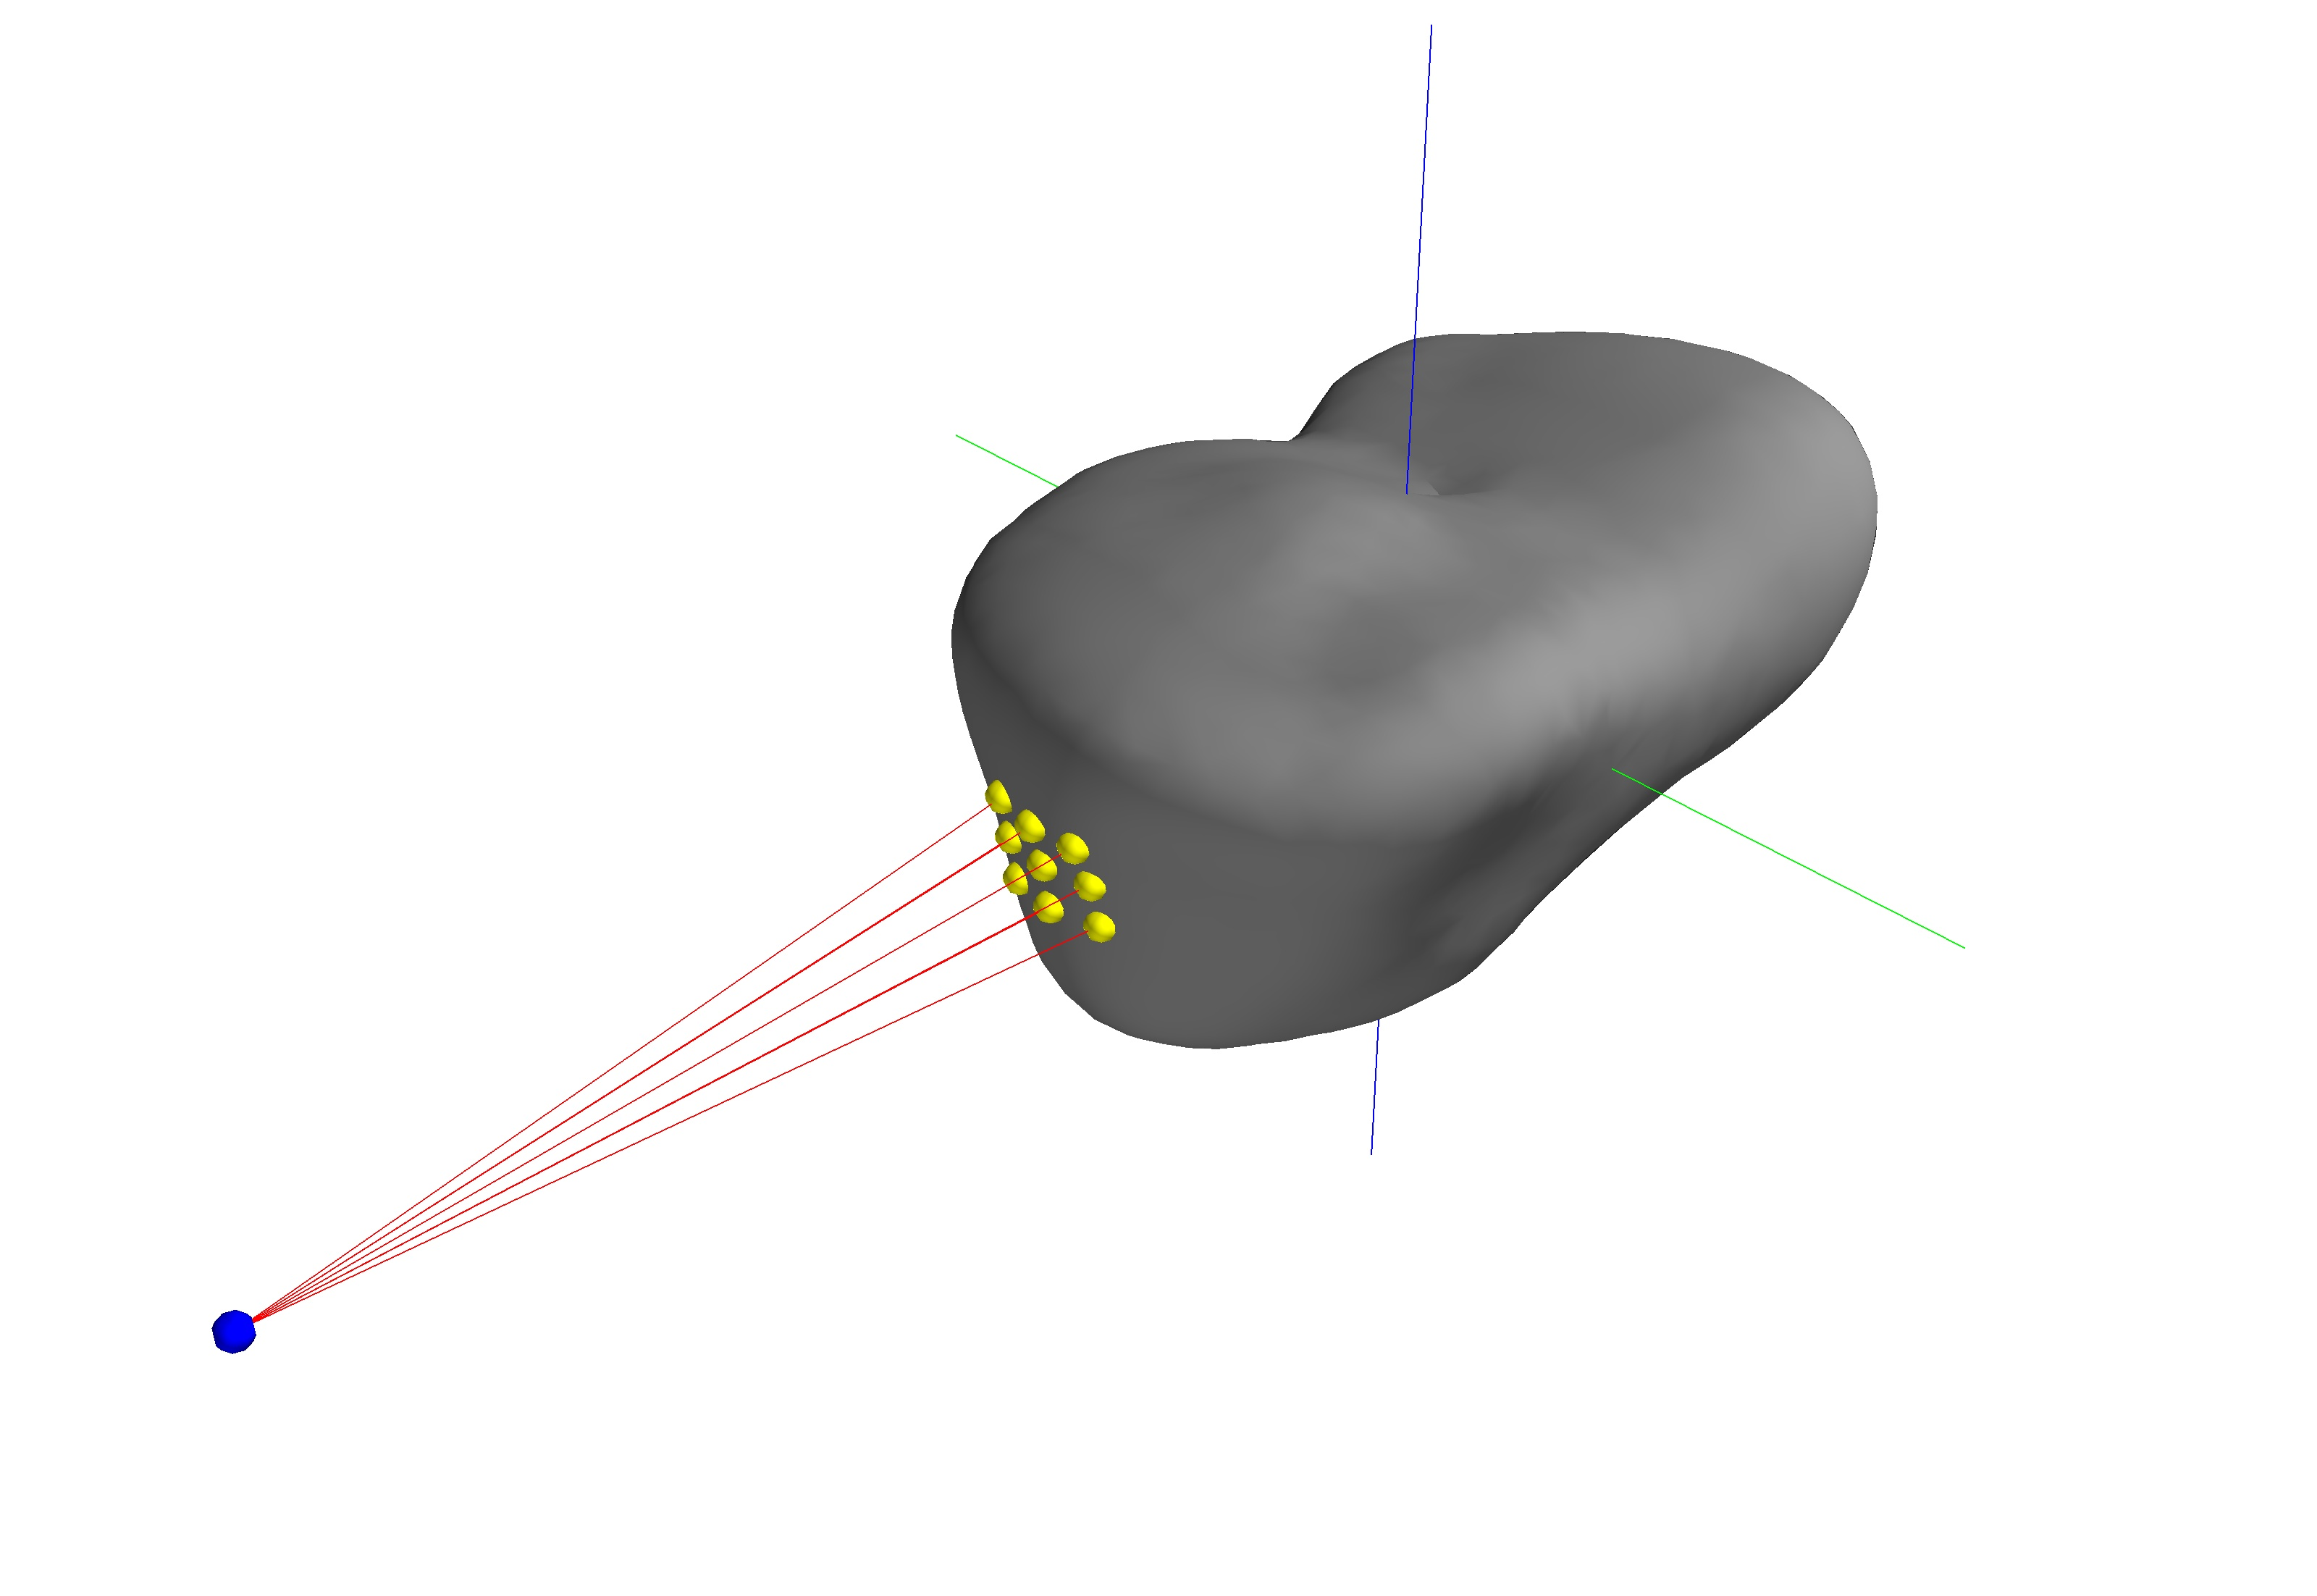
\includegraphics[width=0.75\textwidth,height=0.7\textheight,keepaspectratio]{figures/castalia_raycasting_plot.jpg}
        }
    \end{center}
\end{frame}

\begin{frame}{Bayesian Shape Reconstruction}
    \begin{itemize}
        \item<1-> Framework for combining prior and new data 
            \begin{itemize}
                \item Each vertex has an uncertainty -- \( w_i\) in the radial distance
                \item Each measurement contains error -- \( w_{j, i} \) with respect to each vertex
            \end{itemize}
            \begin{align*}
                v_i \sim \mathcal{N}(r_i, w_i^2) , \quad
                p_{j,i} \sim \mathcal{N}(r_{j,i}, w_{j,i}^2)
            \end{align*}
        \item<2-> New data used to update each vertex and reduce uncertainty
    \begin{align*}\label{eq:posterior_probability}
        \mathcal{N} \parenth{\frac{w_{j, i}^2 r_i + w_i^2 r_{j, i}}{w_i^2 + w_{j, i}^2} , \frac{w_i^2  w_{j, i}^2}{w_i^2 +  w_{j, i}^2}} .
    \end{align*}
    \end{itemize}
\end{frame}

\subsection{Shape Reconstruction}
\begin{frame}{Geographos Reconstruction}
    \begin{itemize}
        \item Potentially hazardous Apollo group asteroid discovered in 1951
    \end{itemize}
    
    \begin{center}
        \href{https://youtu.be/Fy3b80CP2-0}{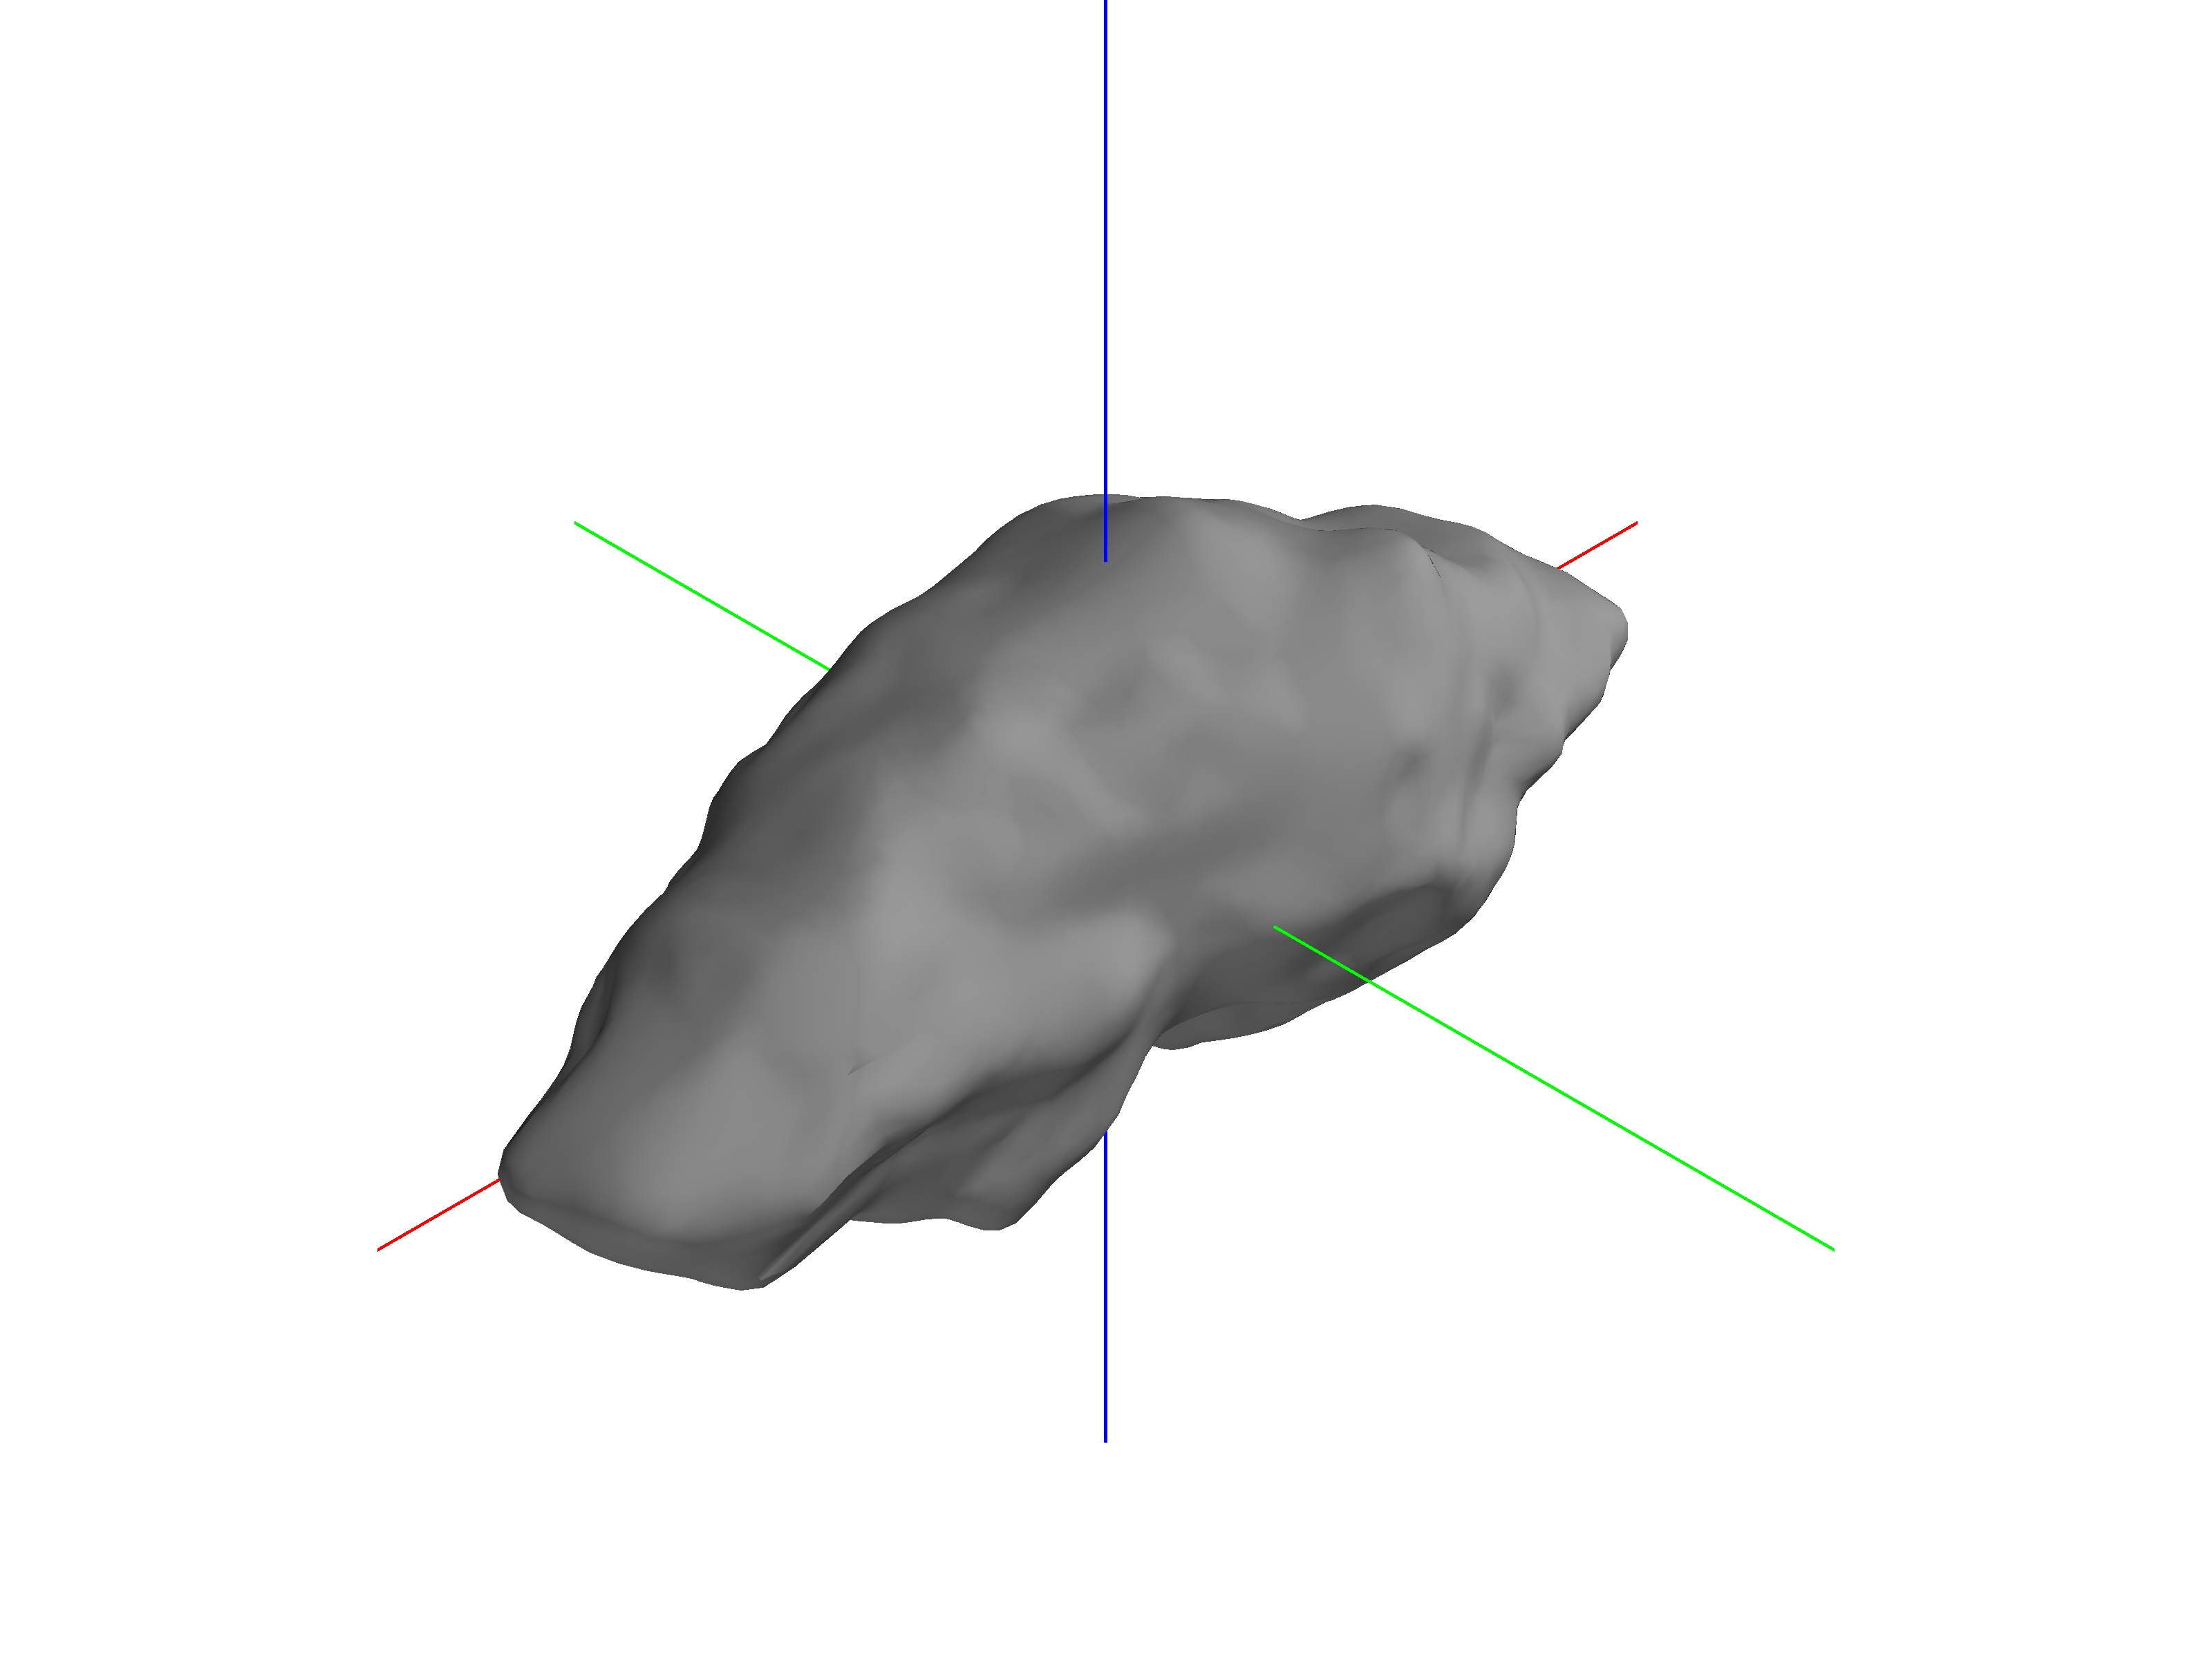
\includegraphics[trim={20cm 15cm 20cm 15cm},clip,keepaspectratio,width=0.5\textwidth]{figures/mesh_update/geographos/partial_7489.jpg}}%
        \href{https://youtu.be/UqISXOuV0ZQ}{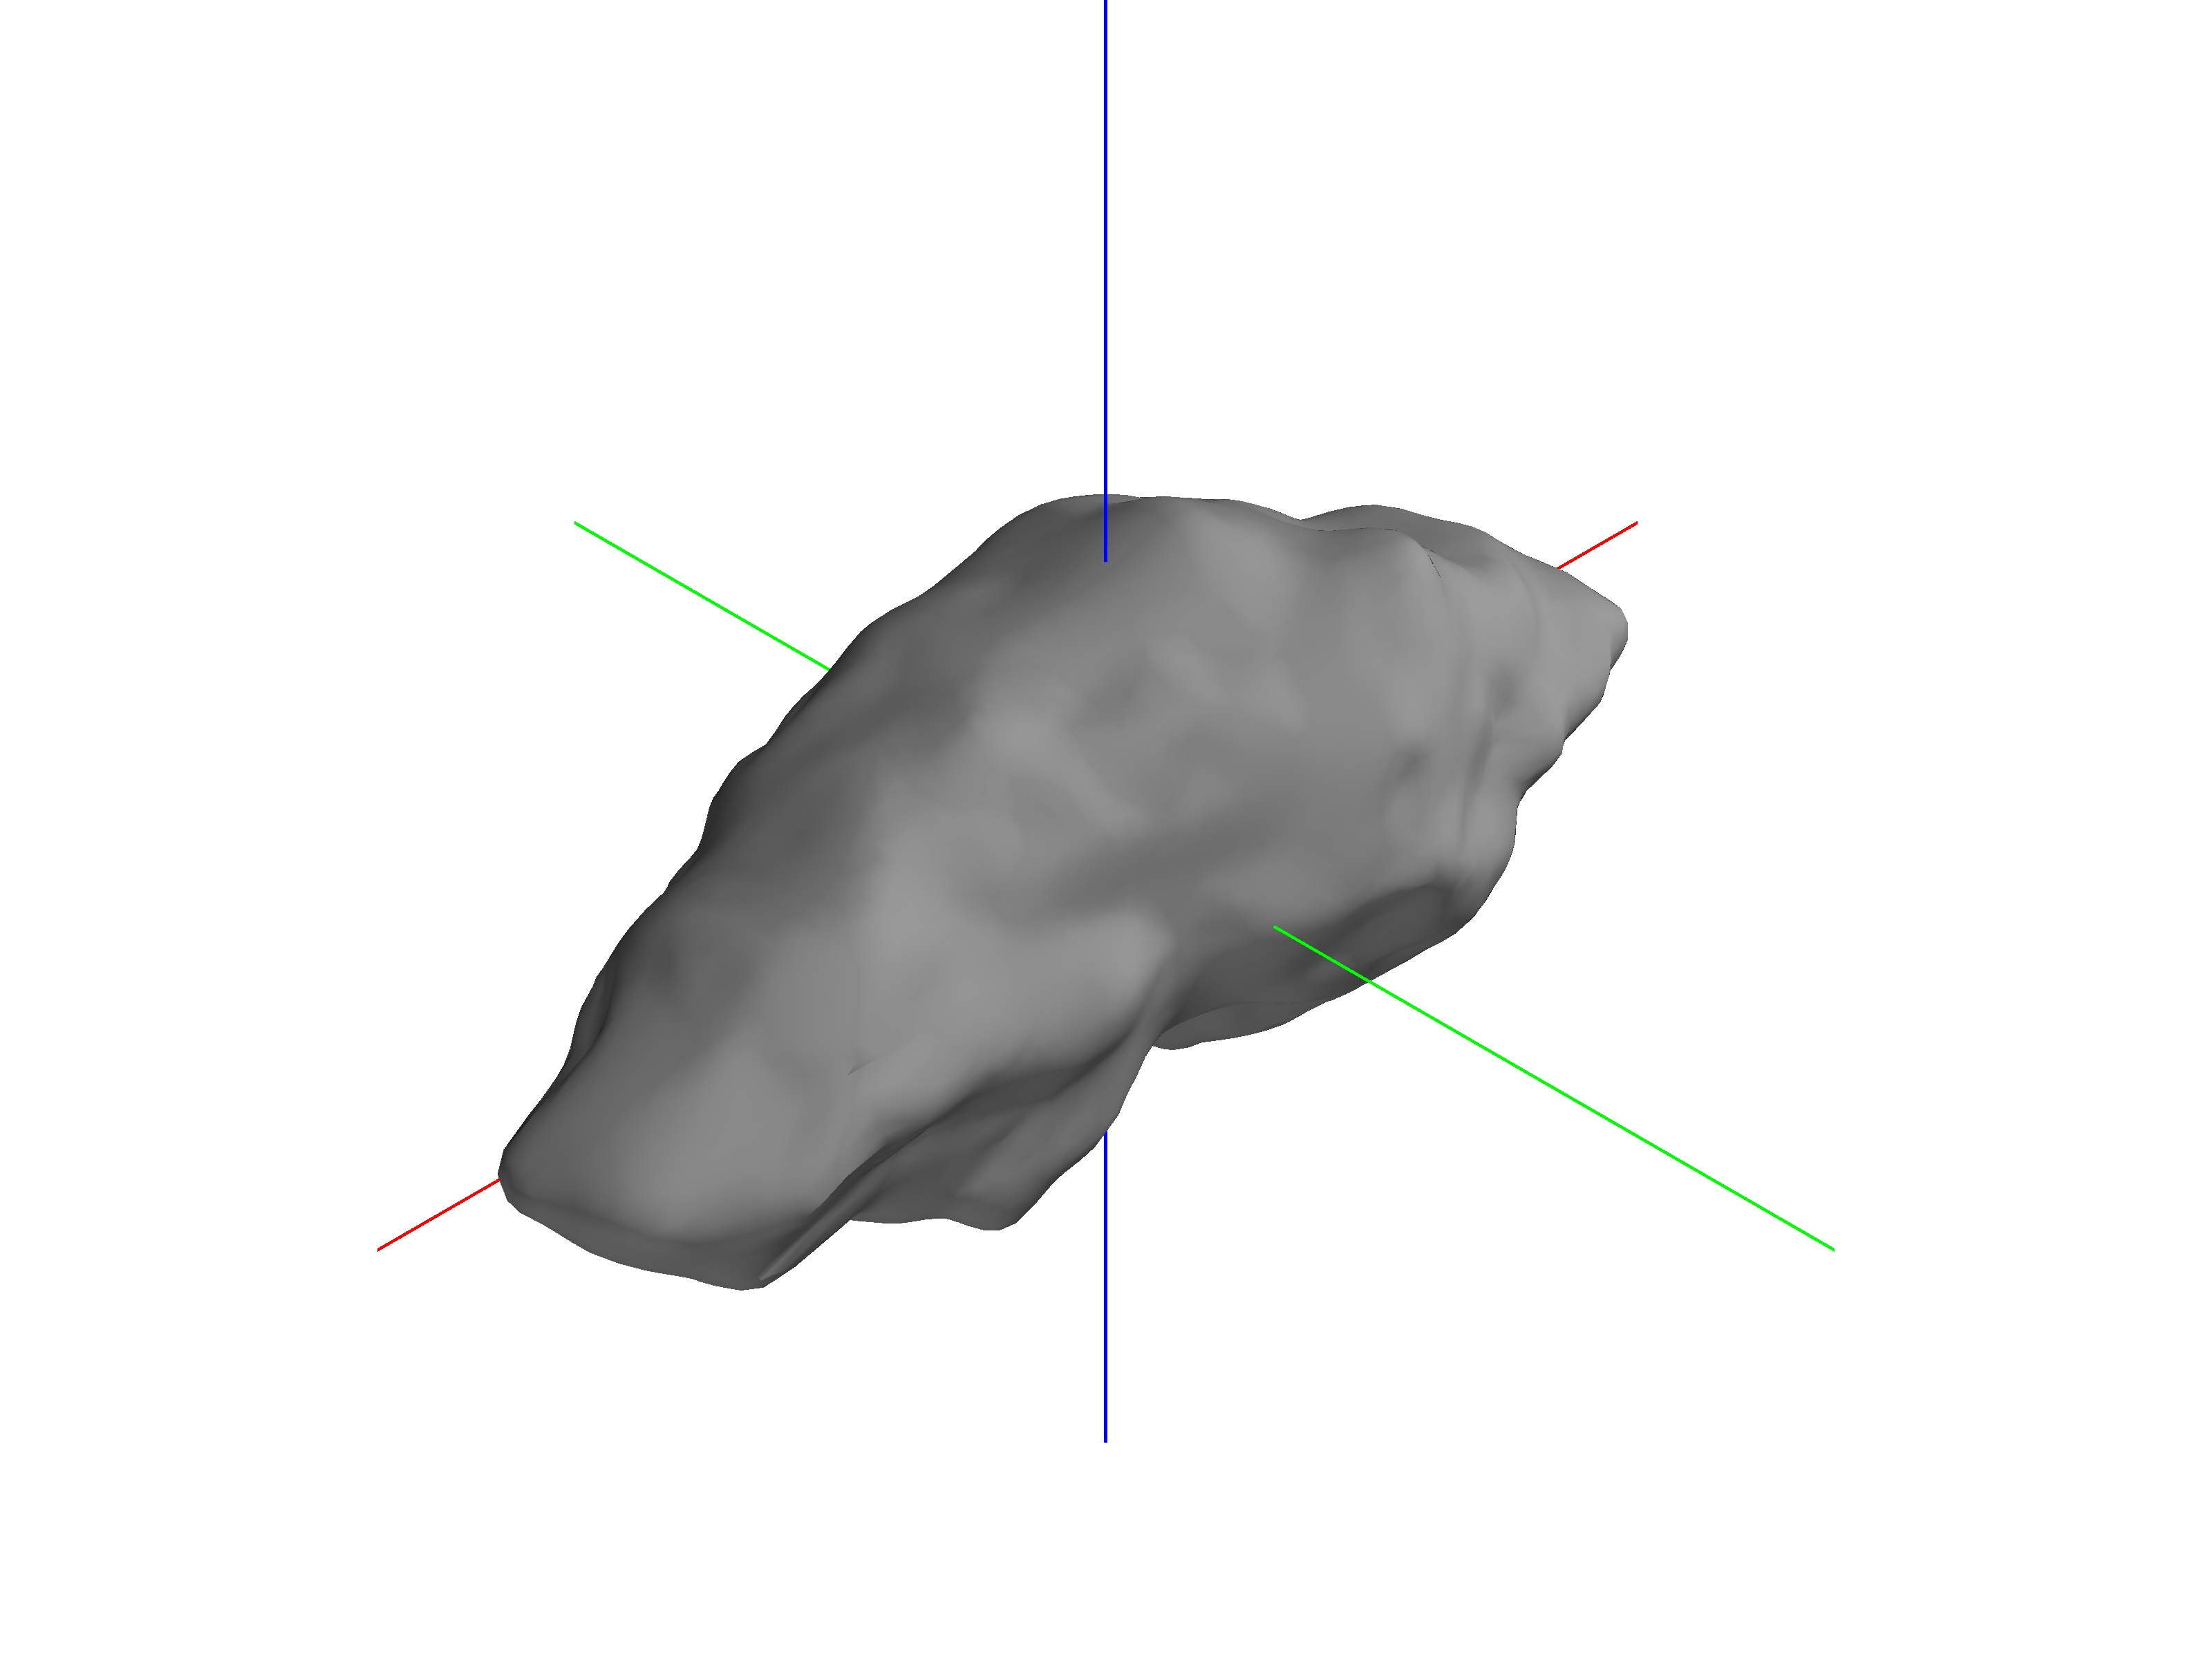
\includegraphics[trim={20cm 15cm 20cm 15cm},clip,keepaspectratio,width=0.5\textwidth]{figures/mesh_update/geographos/partial_7489.jpg}}
\end{center}

\end{frame}

\begin{frame}{Golevka Reconstruction}
    \begin{itemize}
        \item Potentially hazardous Apollo group asteroid discovered in 1995
    \end{itemize}
    \begin{center}
        \href{https://youtu.be/D5JJo1XfOeg}{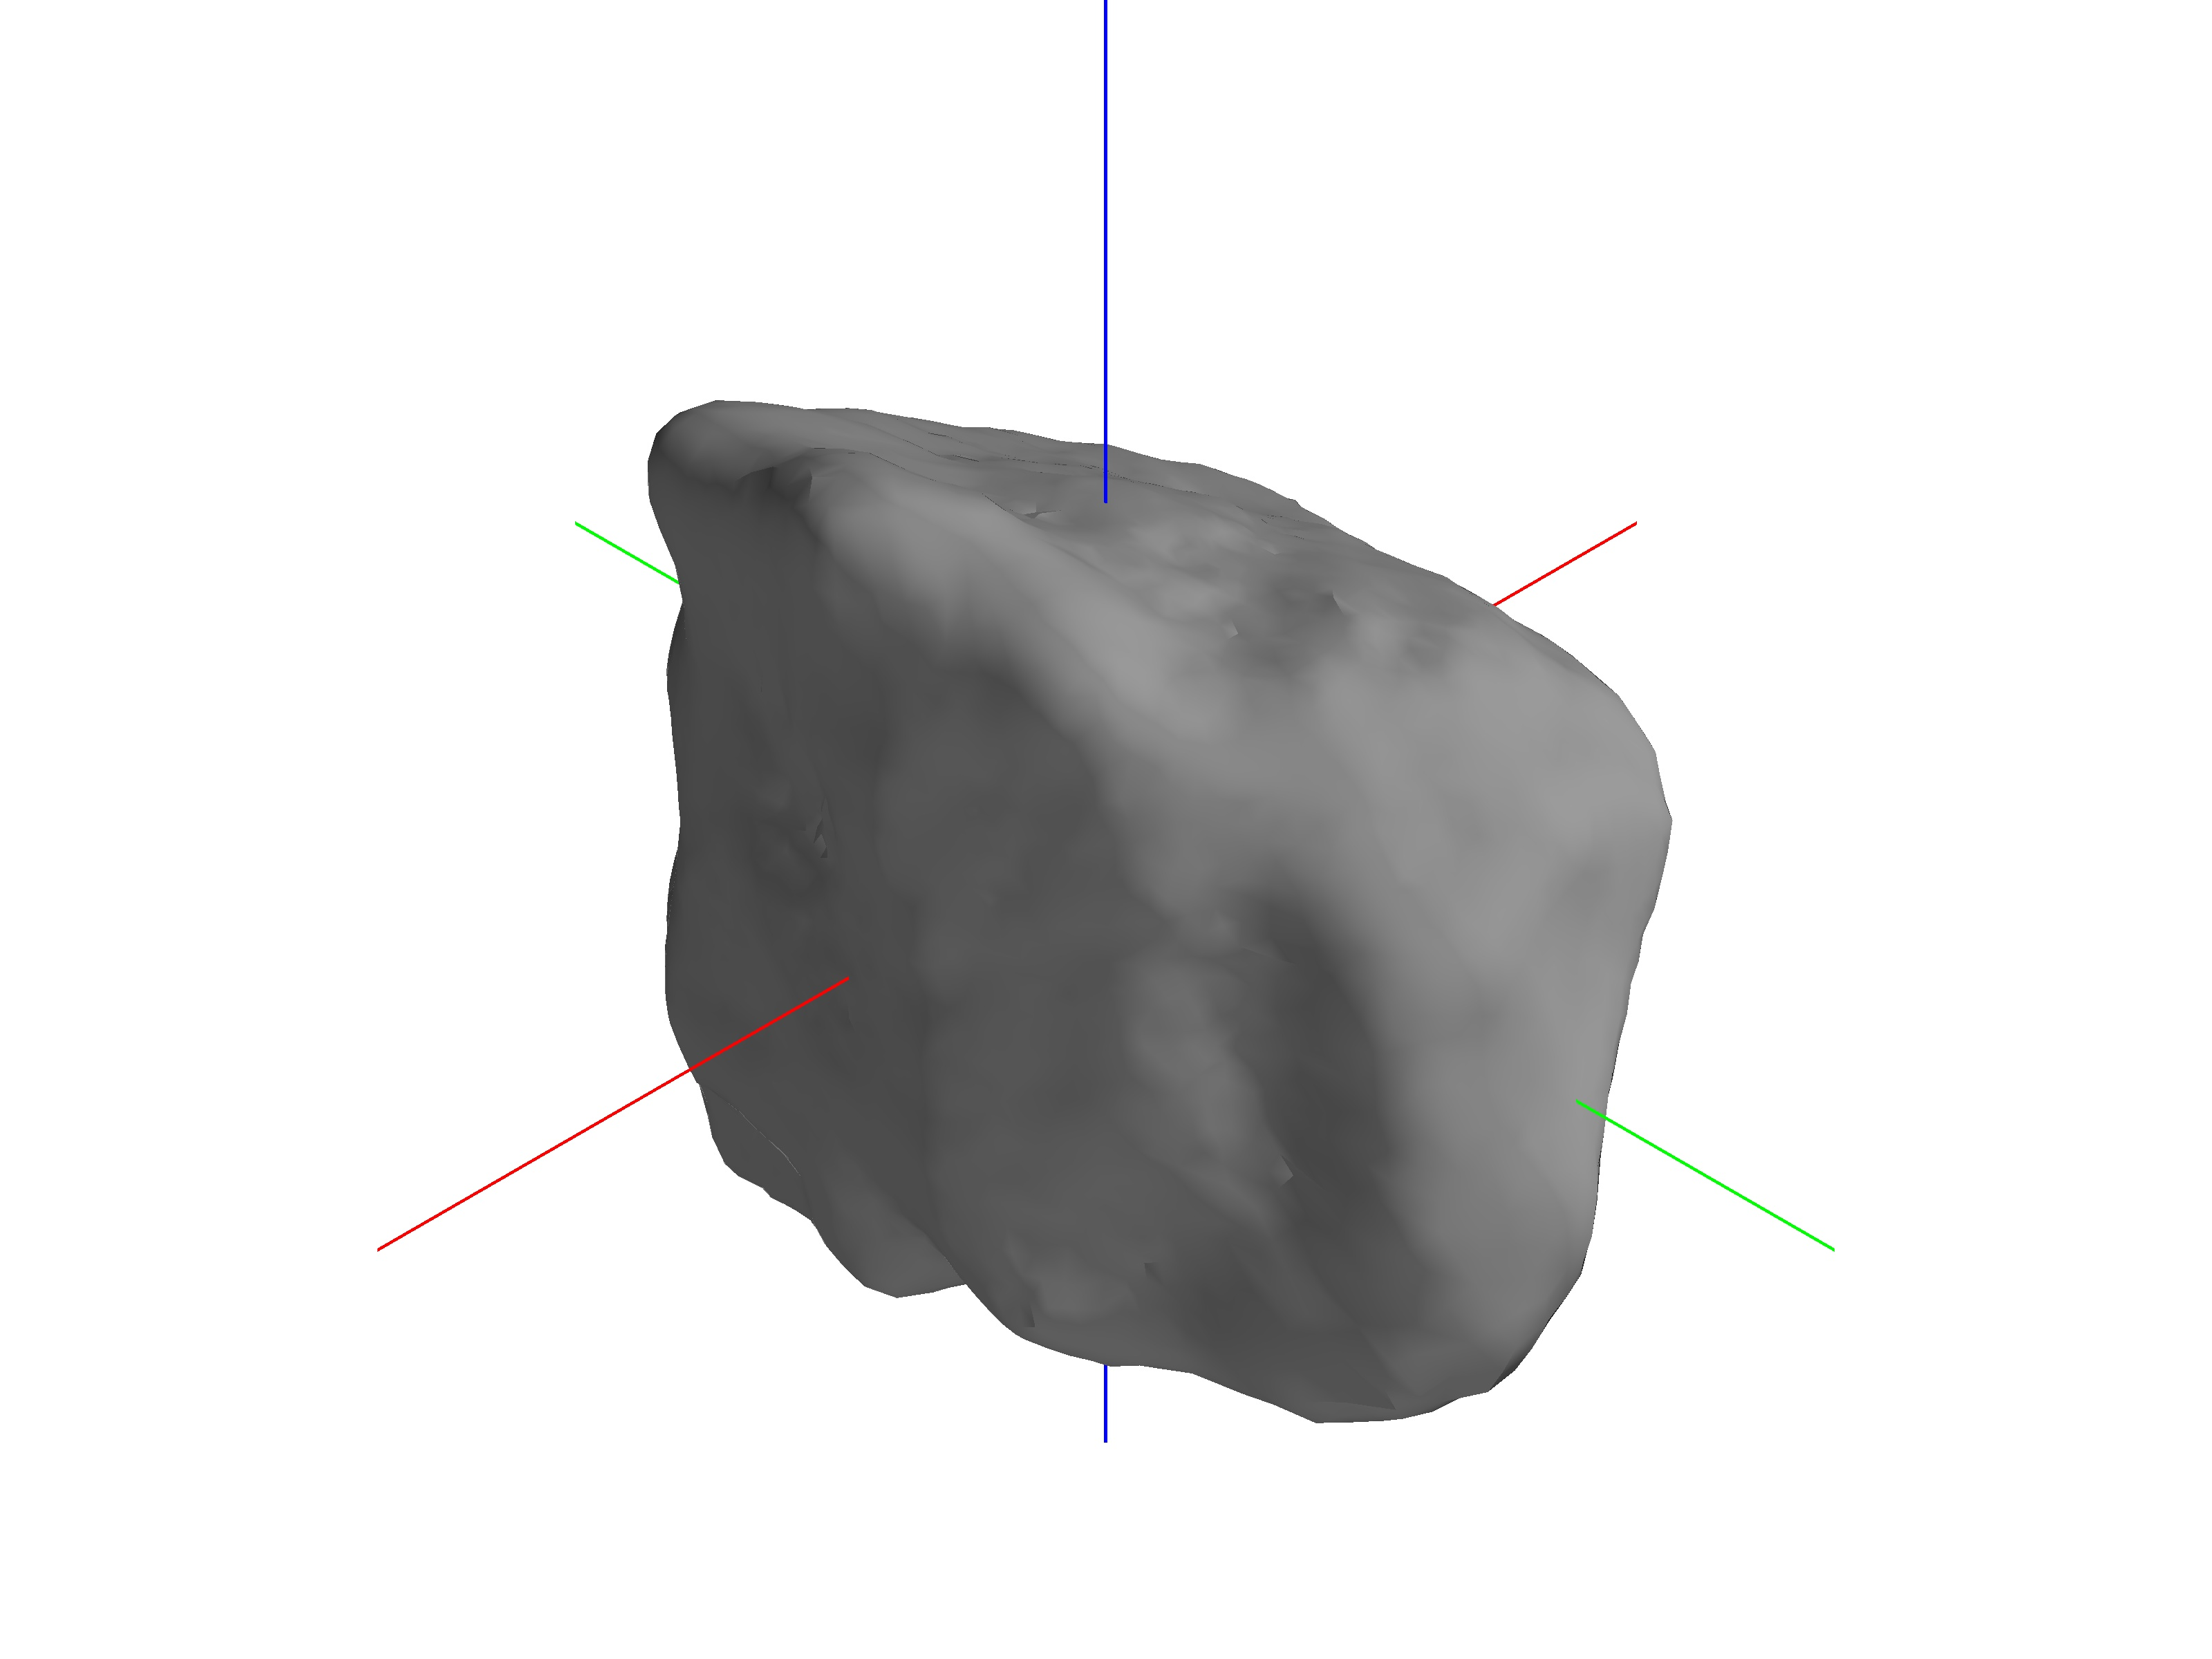
\includegraphics[trim={20cm 10cm 20cm 10cm},clip,keepaspectratio,width=0.5\textwidth]{figures/mesh_update/golevka/partial_5285.jpg}}%
        \href{https://youtu.be/OoaWECewMVI}{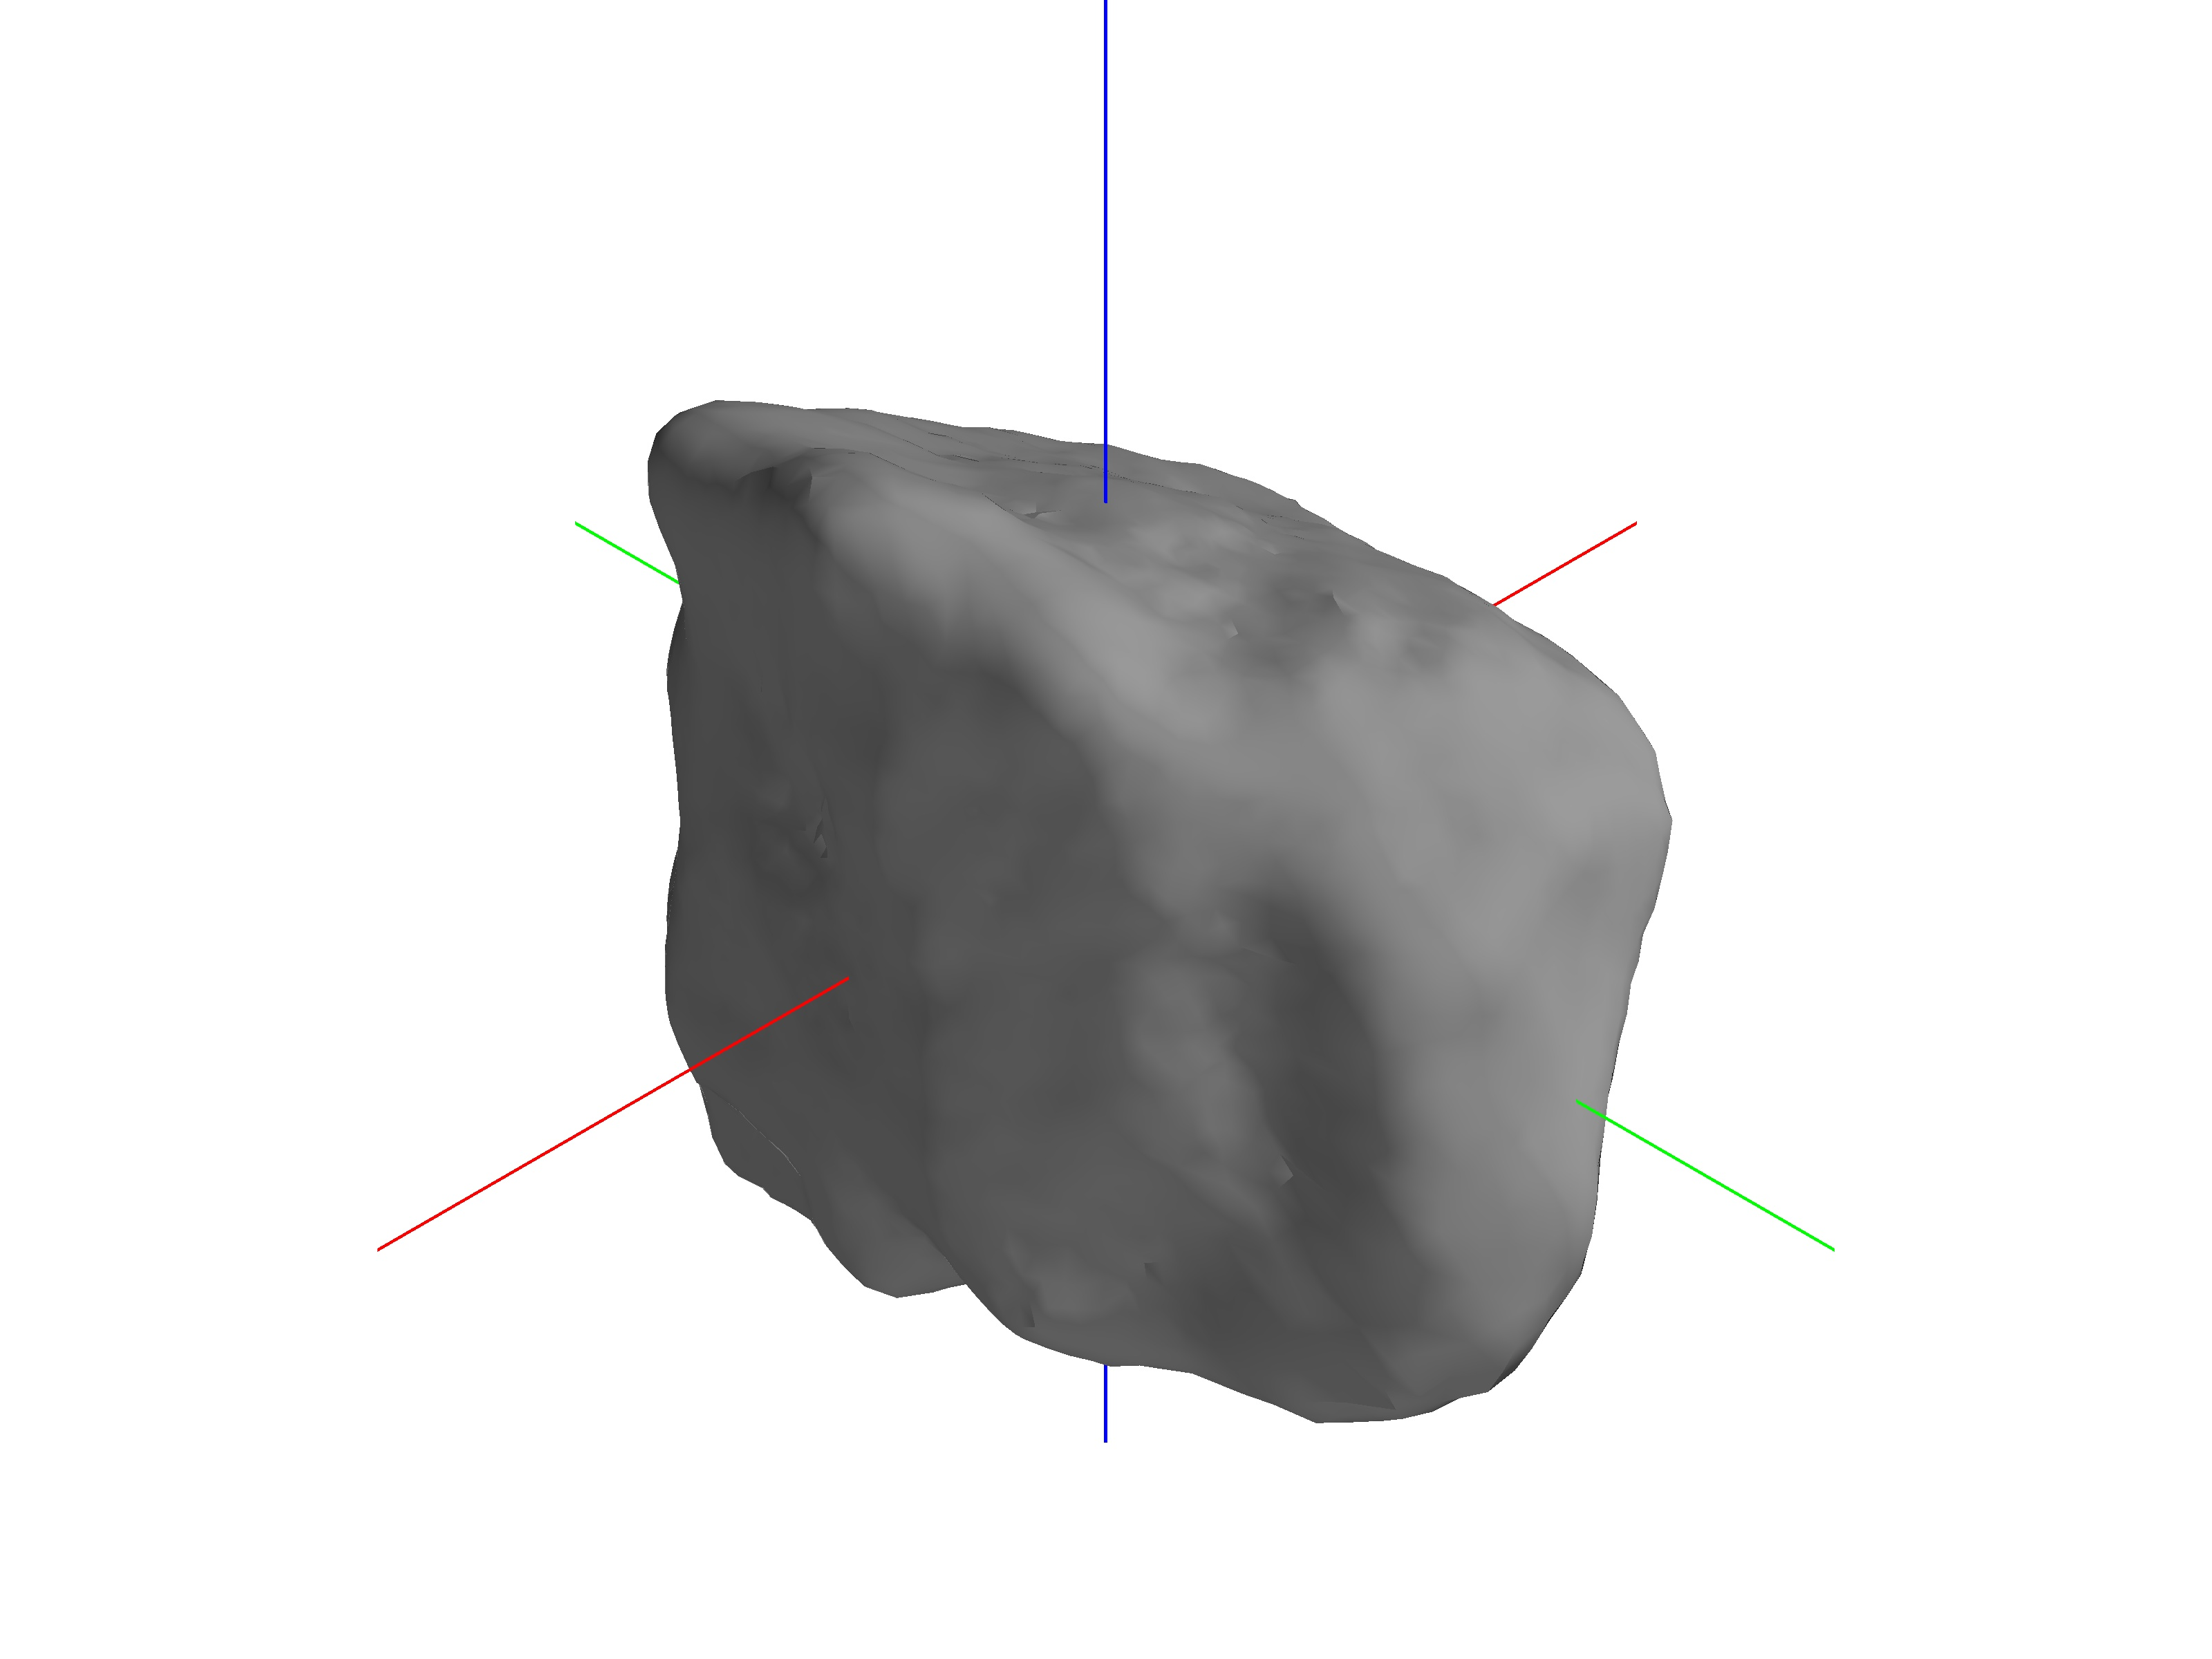
\includegraphics[trim={20cm 10cm 20cm 10cm},clip,keepaspectratio,width=0.5\textwidth]{figures/mesh_update/golevka/partial_5285.jpg}}
\end{center}
\end{frame}

\subsection{Guidance}
\begin{frame}{Optimal Guidance}
    \begin{itemize}
        \item Cost function used to determine future states which provides best measurements
        \item User selected weighting between: uncertainty, distance, and control effort
            % \begin{align*}
            %     J_i (\ipos, \iatt, \aatt) = \alpha_w J_{w_i} + \alpha_d J_{d_i}(\rpos) + \alpha_c J_{c_i}(\rpos)
            % \end{align*}
    \end{itemize}
\begin{center}
        \href{https://youtu.be/ZJY9nPXhyxw}{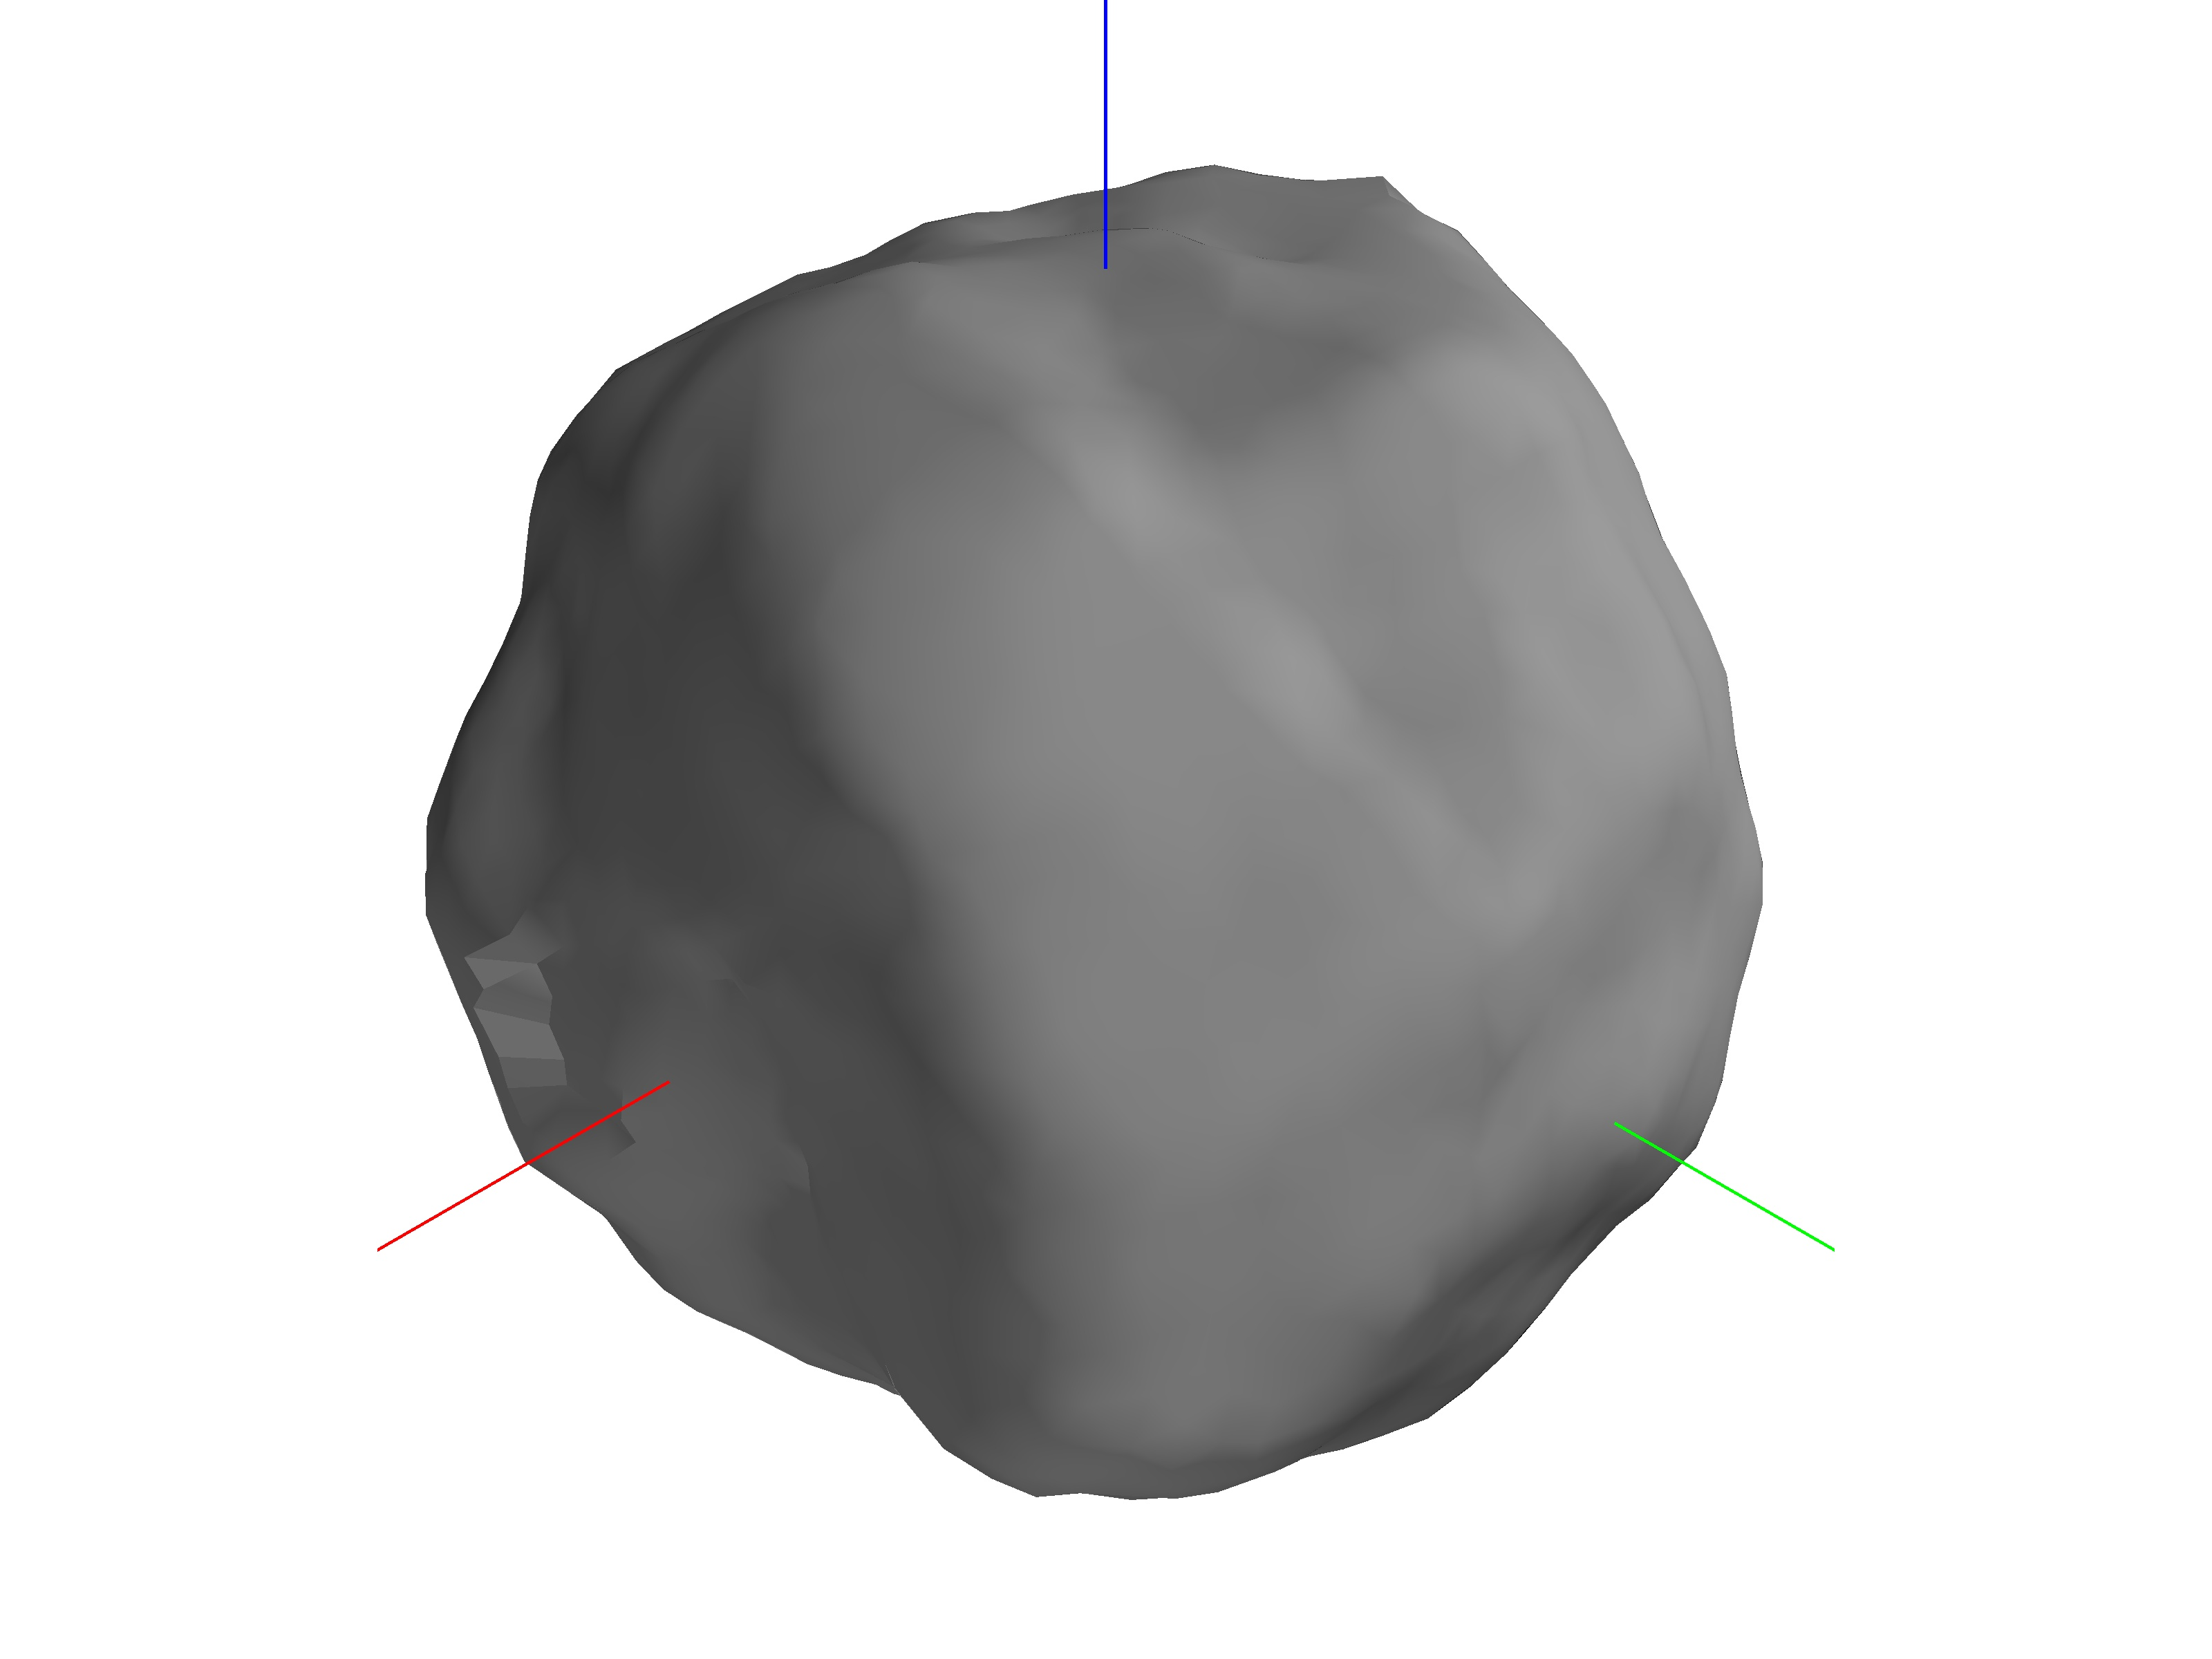
\includegraphics[trim={20cm 8cm 20cm 8cm},clip,keepaspectratio,width=0.5\textwidth,height=0.6\textheight]{figures/dynamic_exploration/52760/partial_14998.jpg}}%
        \href{https://youtu.be/VF8dp8D5nVA}{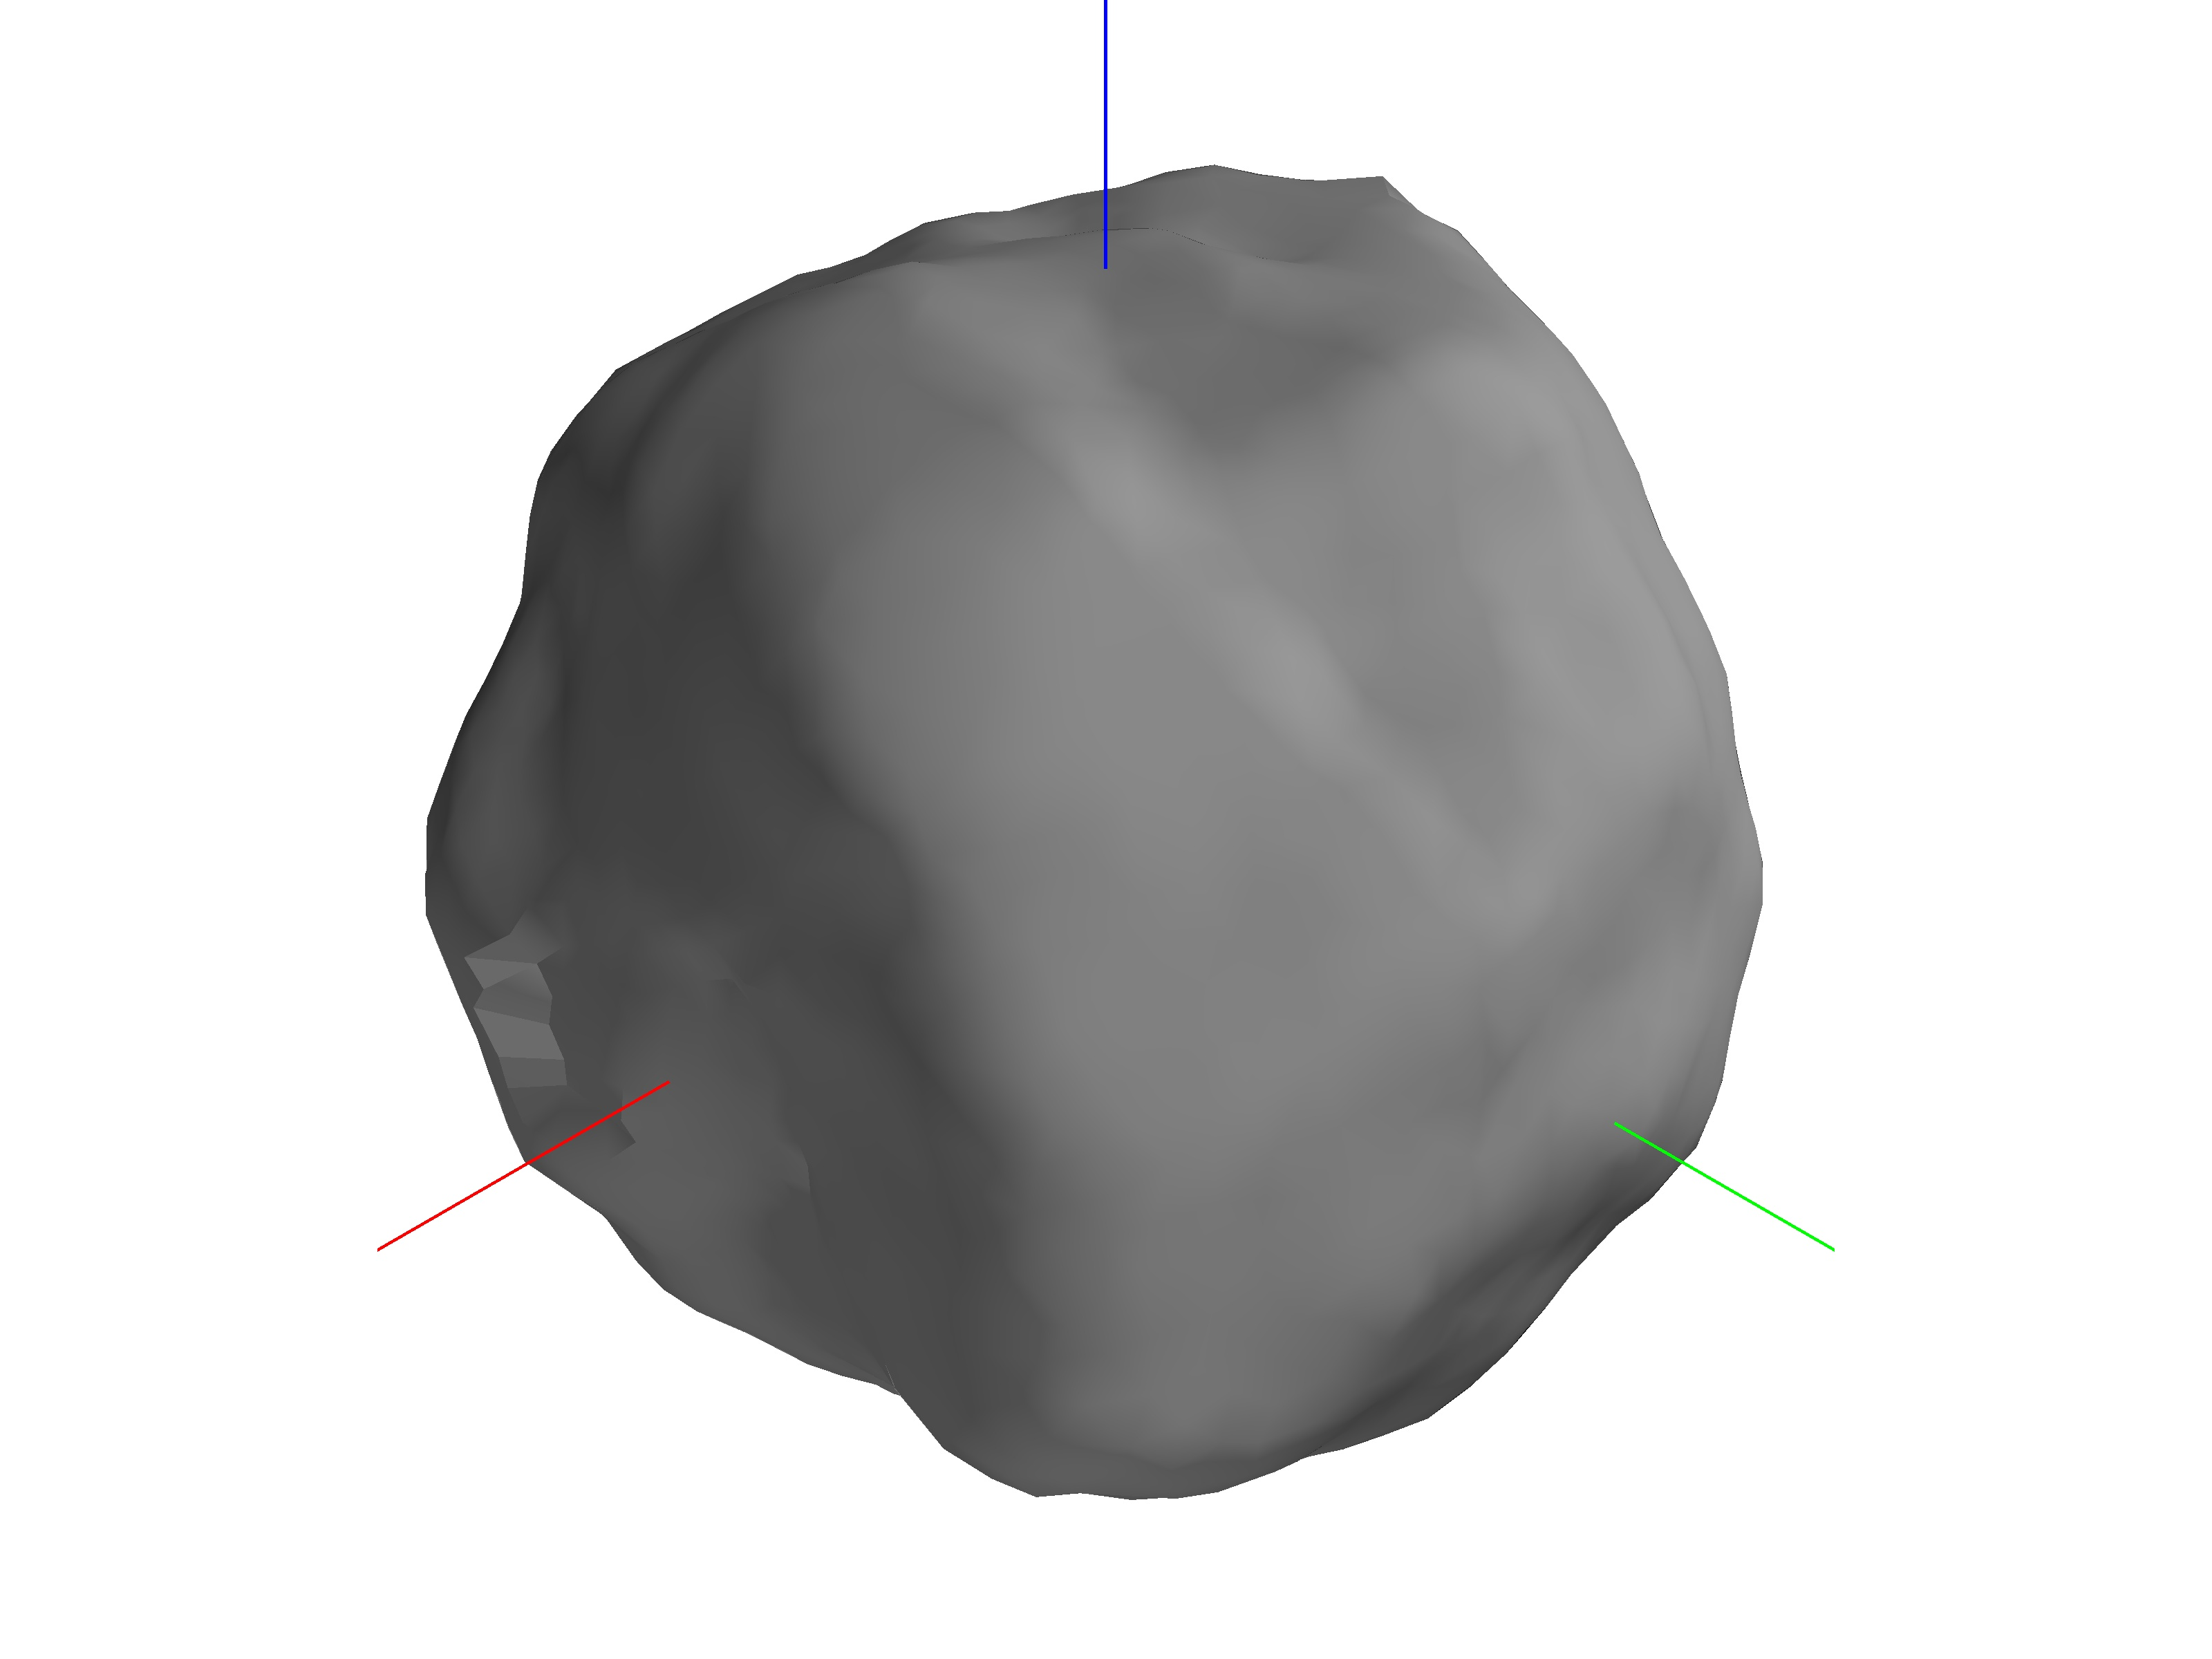
\includegraphics[trim={20cm 8cm 20cm 8cm},clip,keepaspectratio,width=0.5\textwidth,height=0.6\textheight]{figures/dynamic_exploration/52760/partial_14998.jpg}}
\end{center}
\end{frame}

\subsection{Refinement}
\begin{frame}{Landing Site Selection}
    \begin{itemize}
        \item The shape estimate provides sufficient detail to determine the surface slope
            \begin{align*}
                \cos \parenth{ \pi - \phi } = \frac{\vc{n}_f \cdot U_m}{\norm{U_m}},
            \end{align*}
        \item The desired landing area selected to minimize: slope and distance
        \item Desired landing area used for multi-resolution refinement
    \end{itemize}
    \pause
    \begin{center}
        \only<1>{
        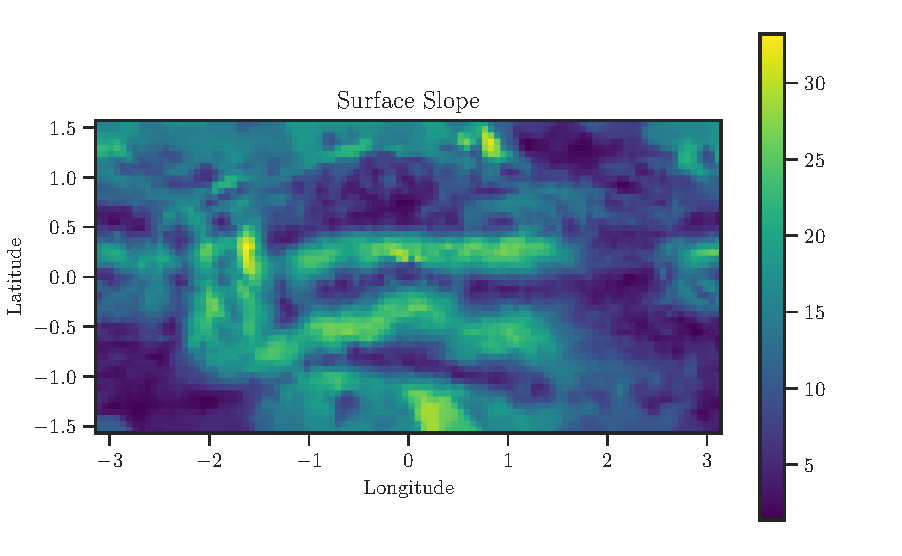
\includegraphics[width=0.5\textwidth]{figures/dynamic_exploration/castalia/refine/slope.pdf}%
        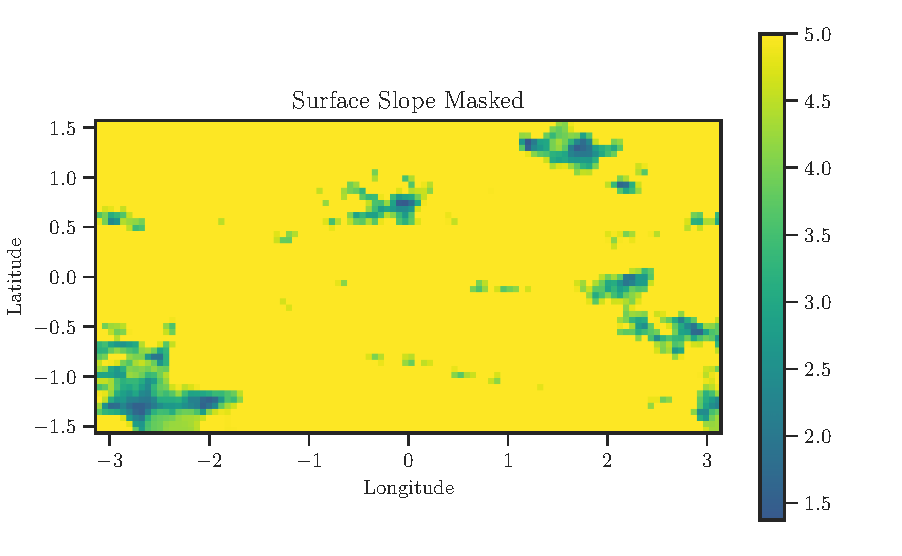
\includegraphics[width=0.5\textwidth,keepaspectratio]{figures/dynamic_exploration/castalia/refine/slope_masked.pdf}
    }
    \only<2>{
        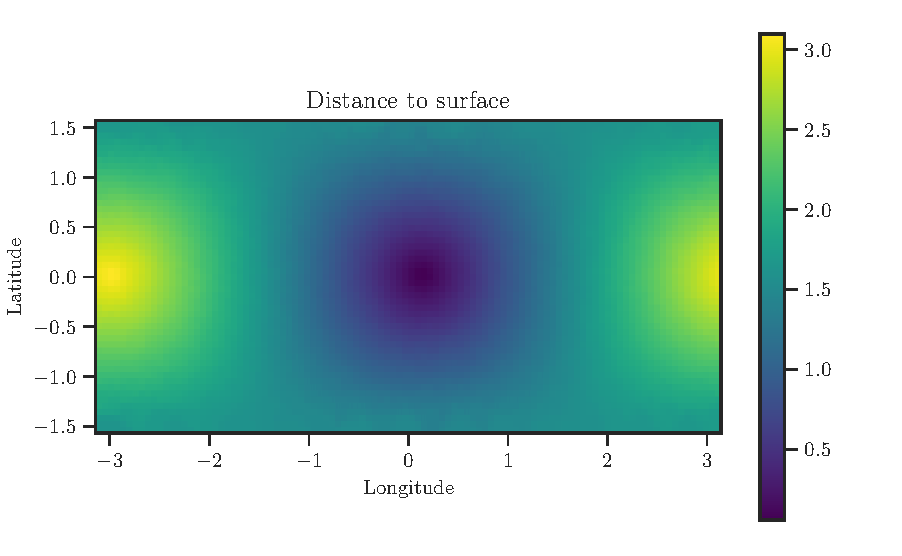
\includegraphics[width=0.5\textwidth]{figures/dynamic_exploration/castalia/refine/dist.pdf}%
        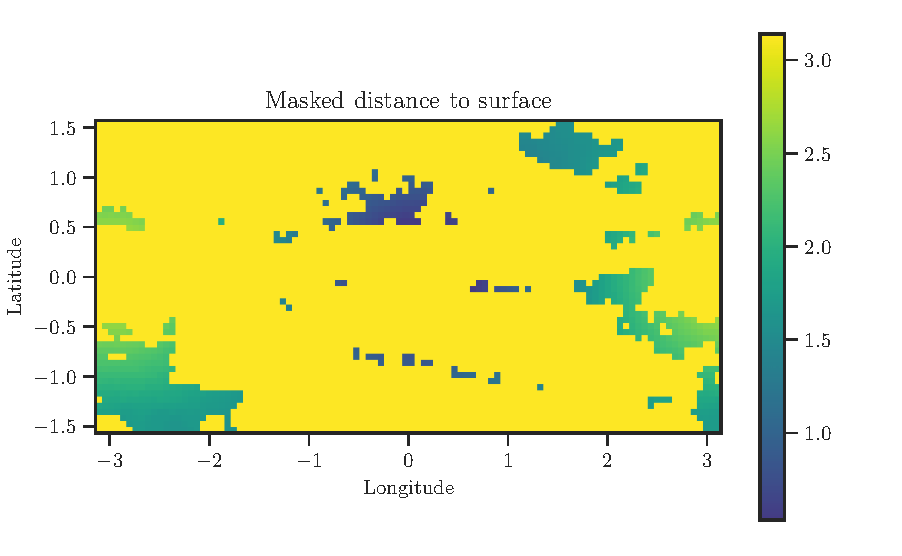
\includegraphics[width=0.5\textwidth,keepaspectratio]{figures/dynamic_exploration/castalia/refine/dist_masked.pdf}
    }
    \only<3>{
        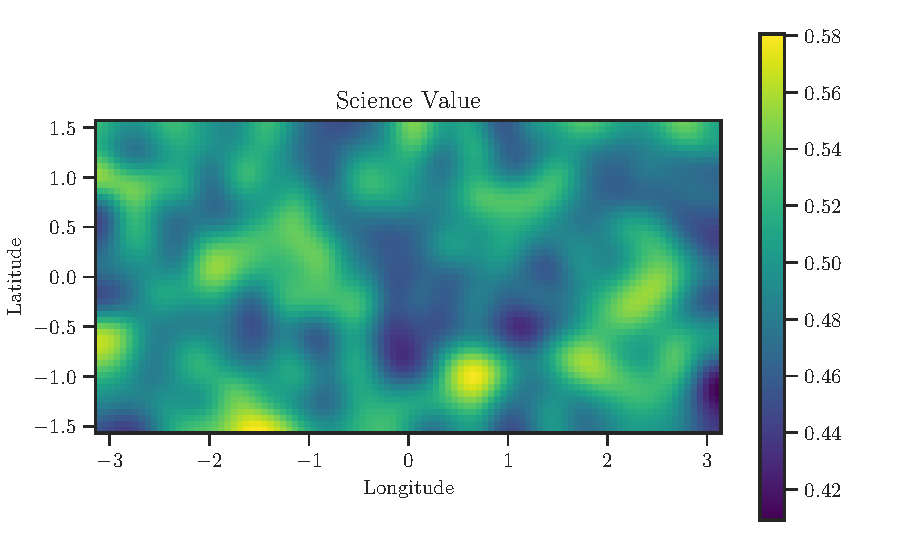
\includegraphics[width=0.5\textwidth]{figures/dynamic_exploration/castalia/refine/science.pdf}%
        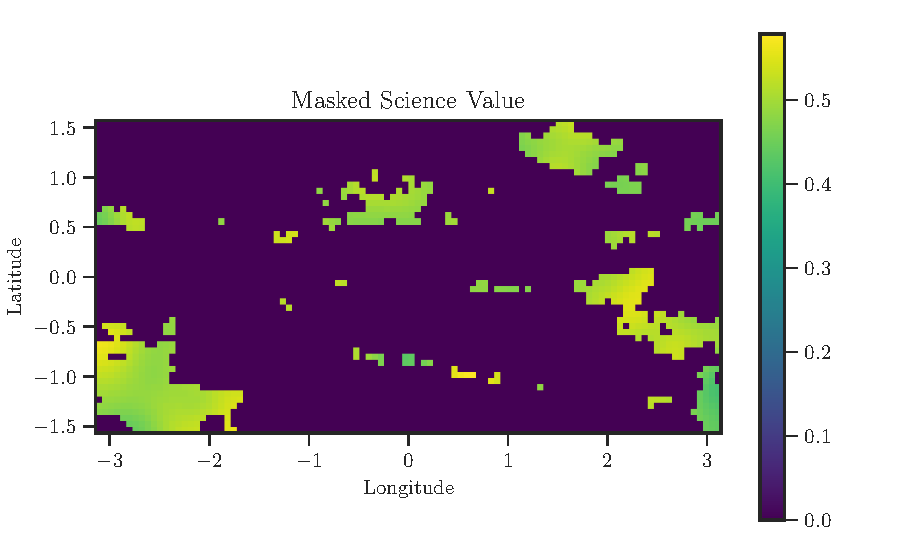
\includegraphics[width=0.5\textwidth,keepaspectratio]{figures/dynamic_exploration/castalia/refine/science_masked.pdf}
    }
    \only<4>{
        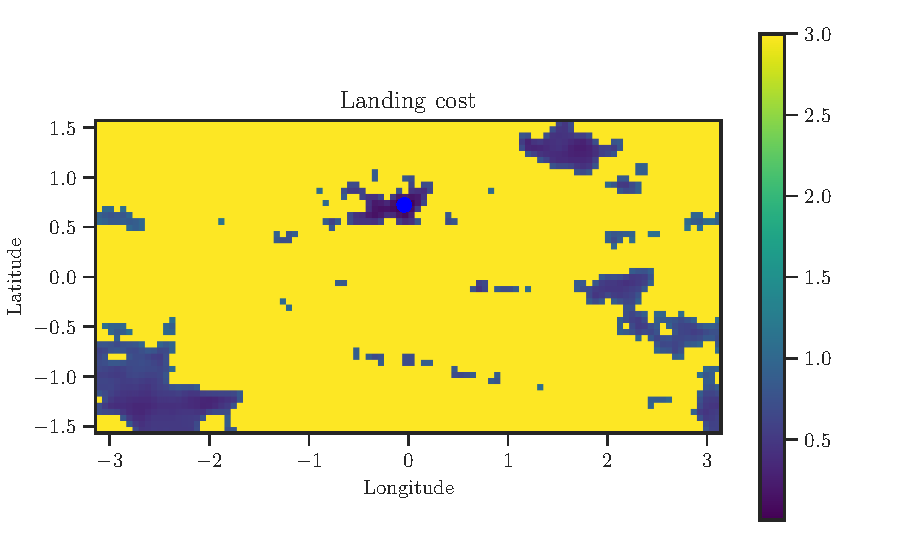
\includegraphics[width=0.5\textwidth]{figures/dynamic_exploration/castalia/refine/cost.pdf}%
    }
    \end{center}
\end{frame}

\begin{frame}{Multi-resolution Refinement}
    \begin{itemize}
        \item The mesh resolution limits the size of captured features
        \item A uniform high resolution mesh would be computationally intractable
    \end{itemize}
    \begin{center}%
        \only<1>{
            
\includegraphics[height=0.7\textheight]{figures/isotropic/original_cube.jpg}%
            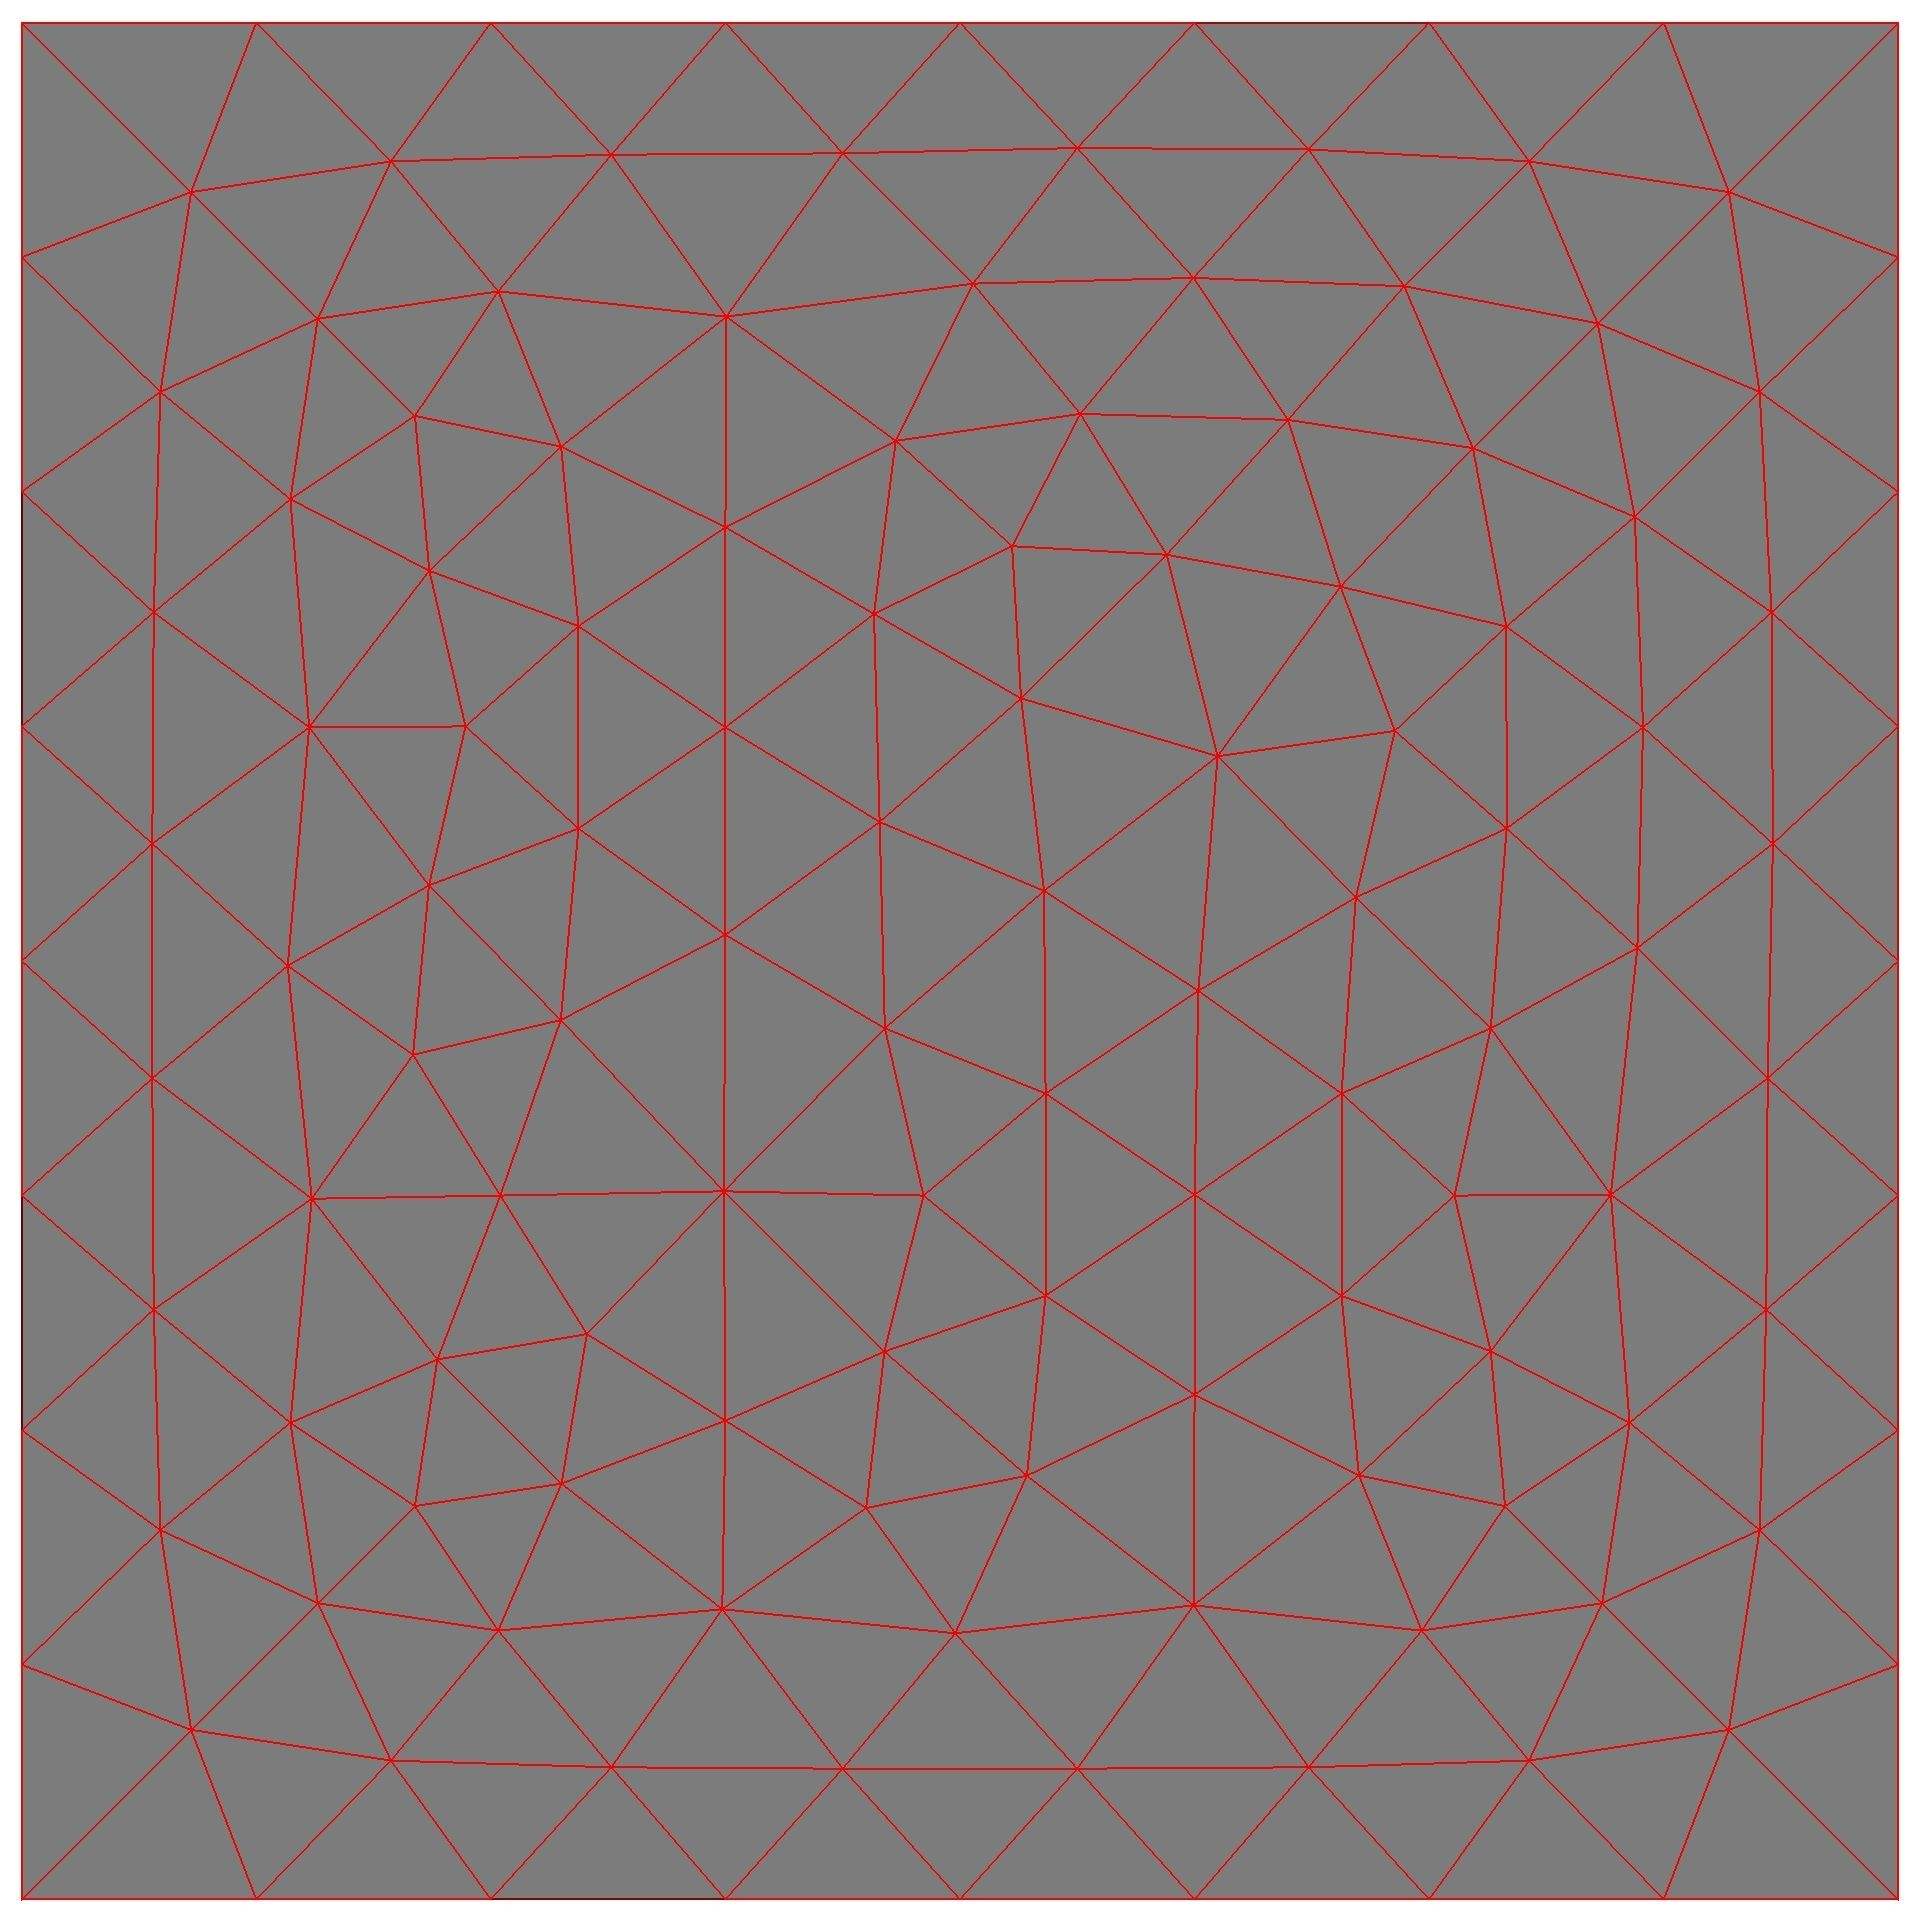
\includegraphics[height=0.7\textheight]{figures/isotropic/remesh_cube.jpg}
        }
        \only<2>{
            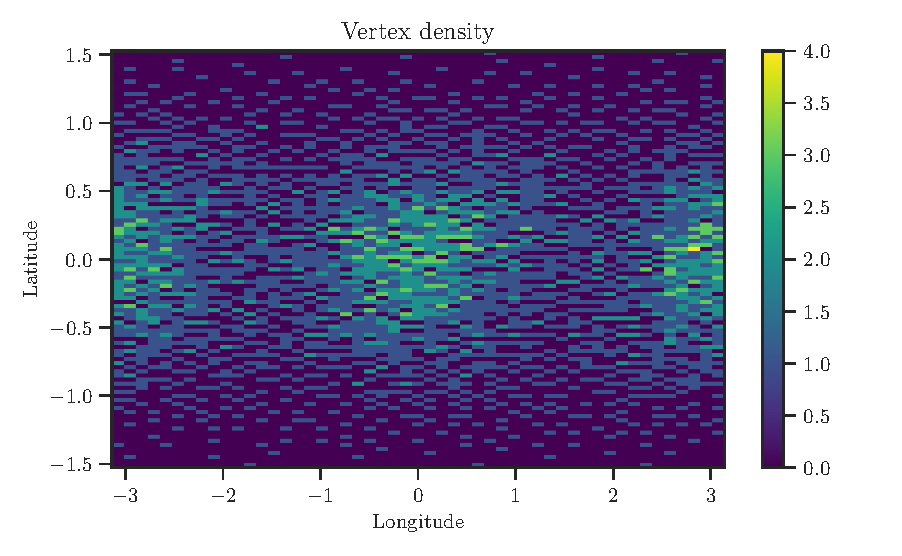
\includegraphics[height=0.7\textheight]{figures/dynamic_exploration/castalia/refine/density.pdf}
        }
        \only<3>{
            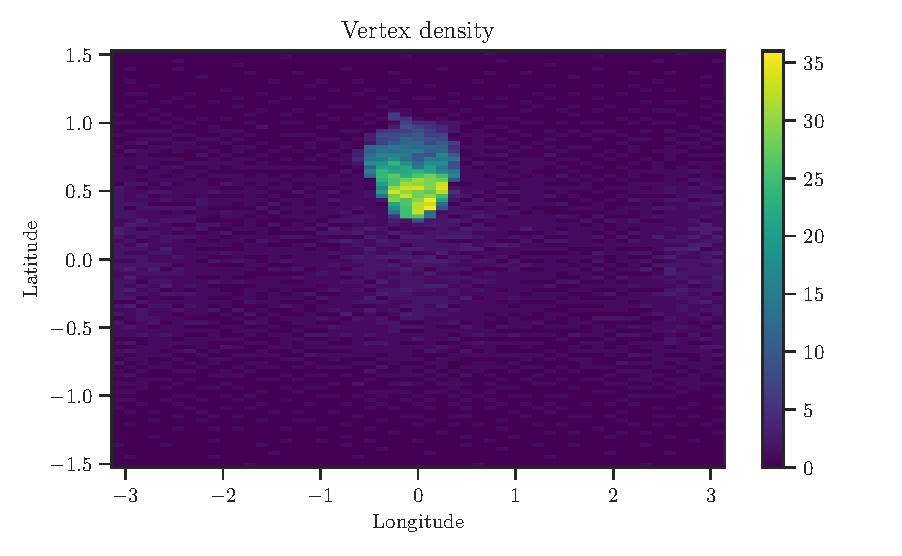
\includegraphics[height=0.7\textheight]{figures/dynamic_exploration/castalia/land/density.pdf}
        }
    \end{center}
\end{frame}

\begin{frame}{4769 Castalia Exploration}

\begin{center}
    \href{https://youtu.be/EMlYvBGN8S0}{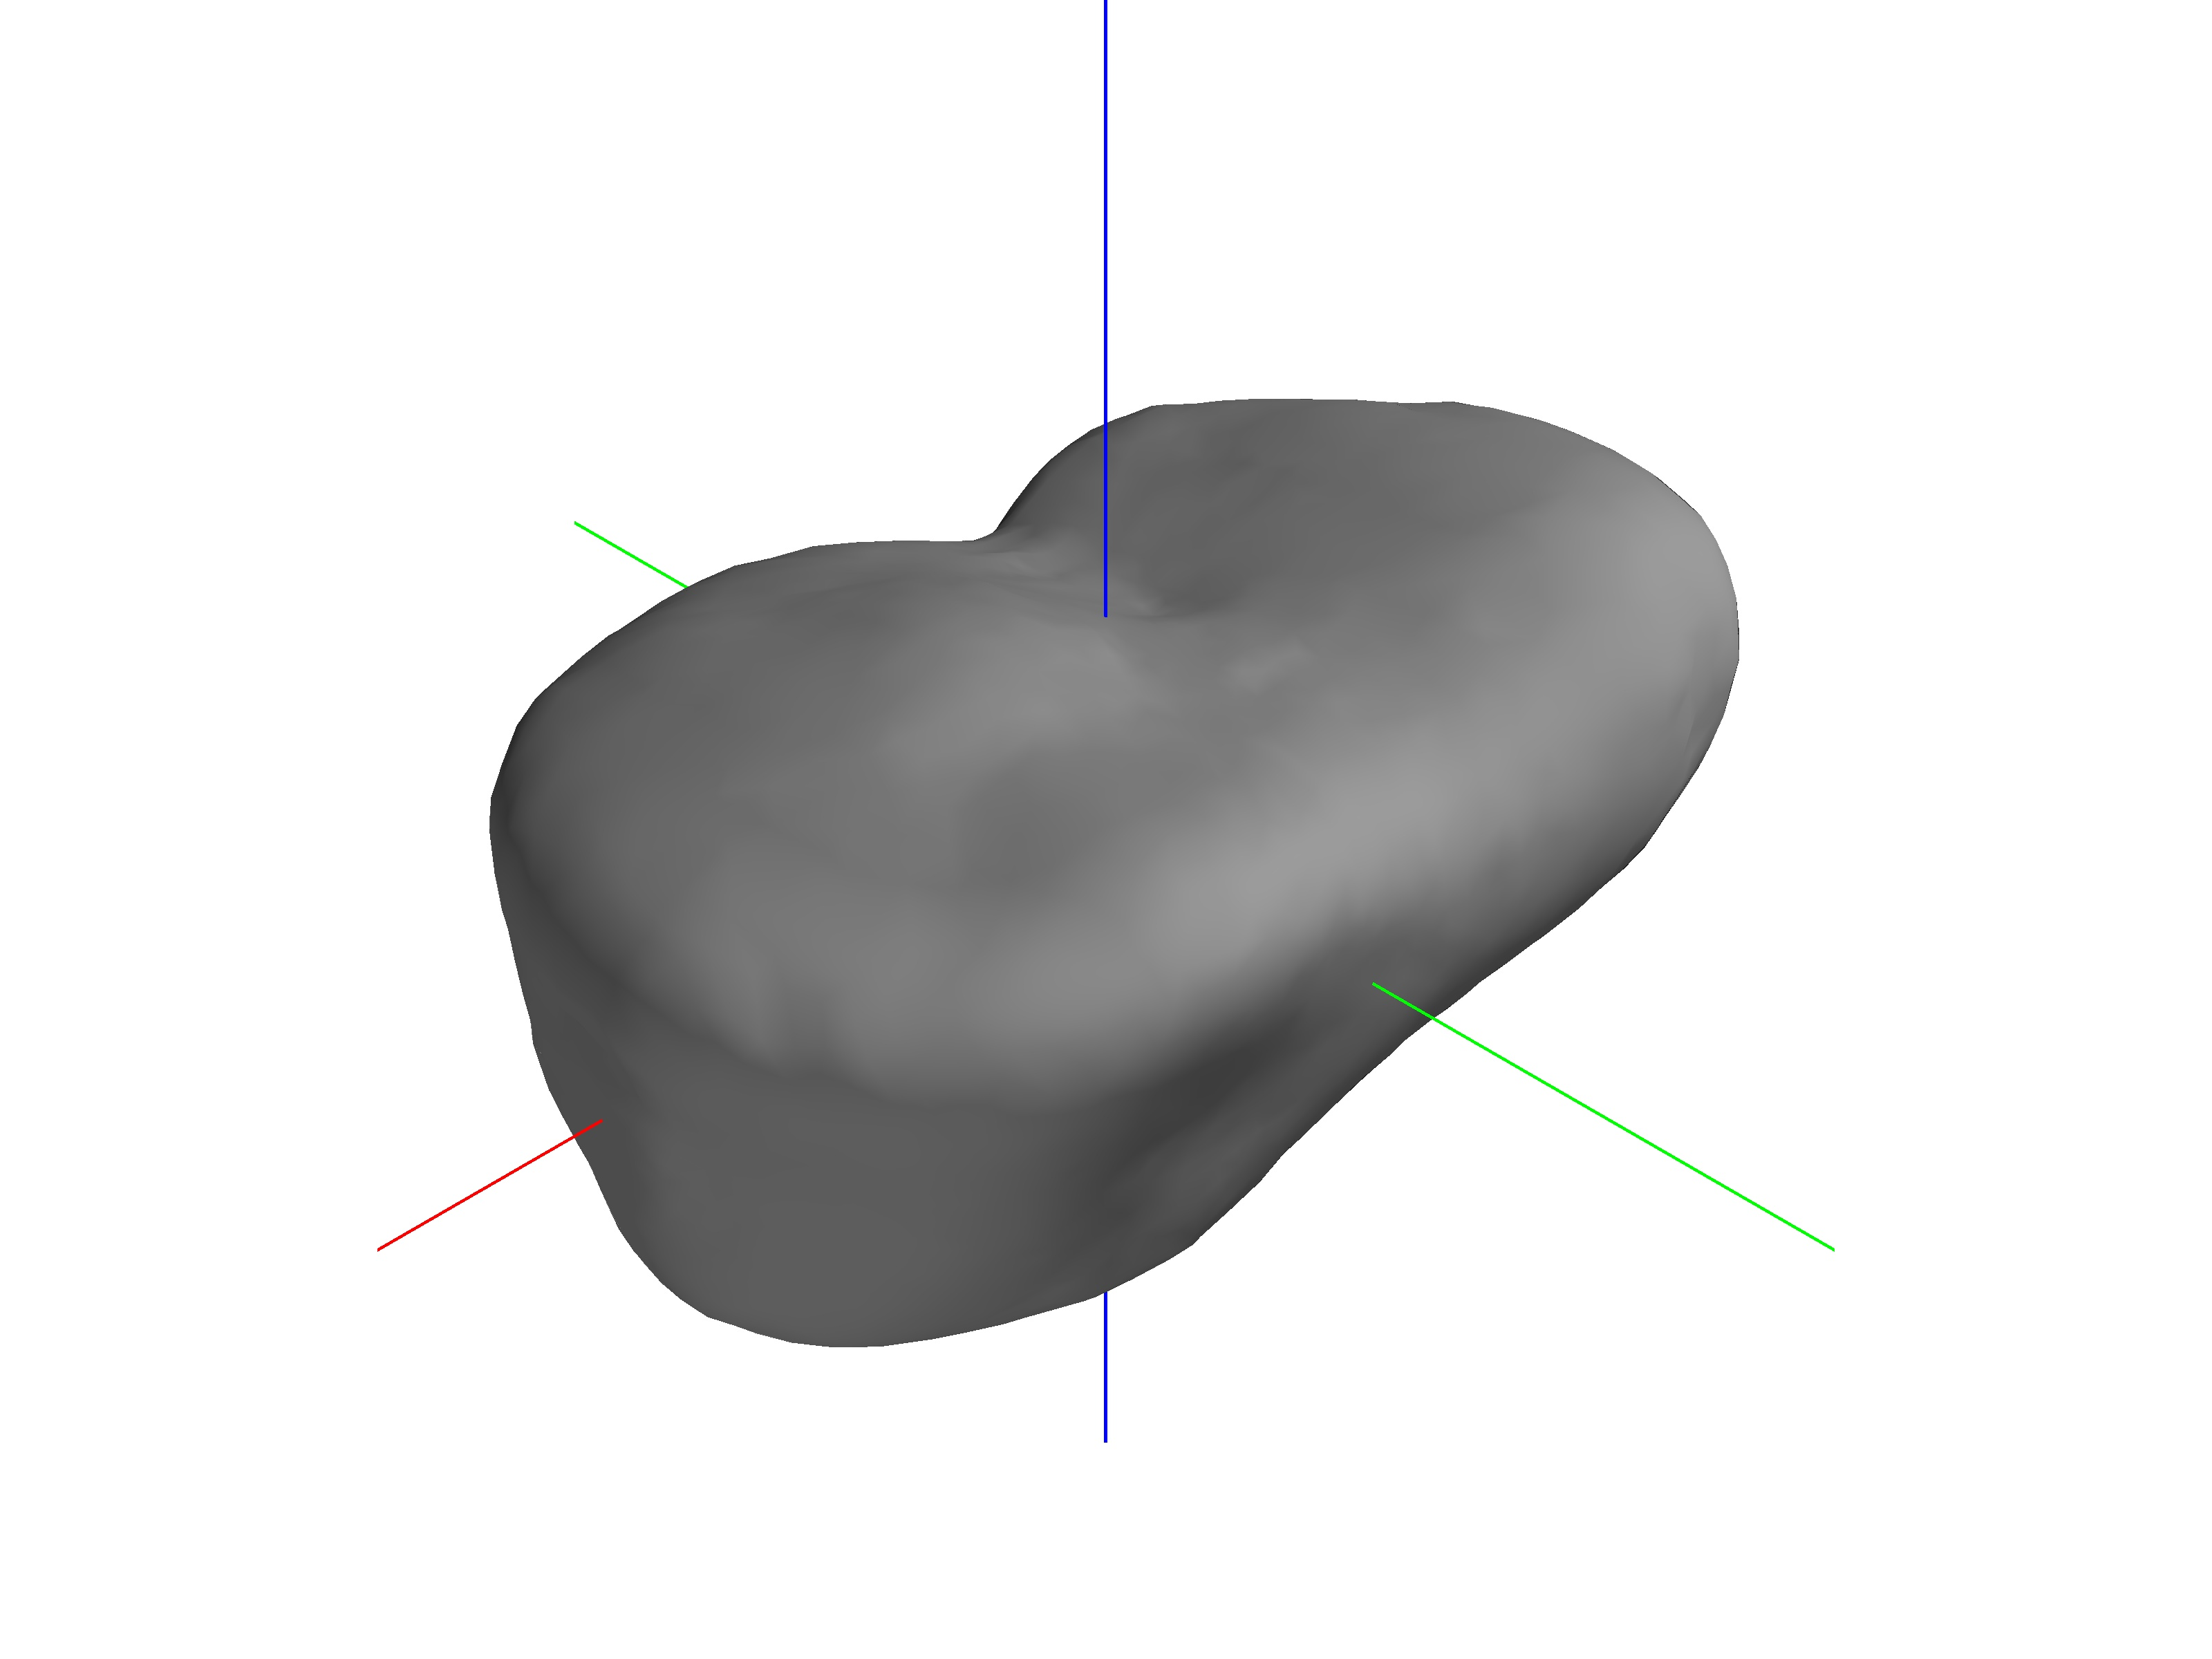
\includegraphics[trim={20cm 10cm 20cm 10cm},clip,keepaspectratio,width=0.5\textwidth,height=\textheight]{figures/dynamic_exploration/castalia/partial_14998.jpg}}%
        \href{https://youtu.be/jz-_SIi4a5A}{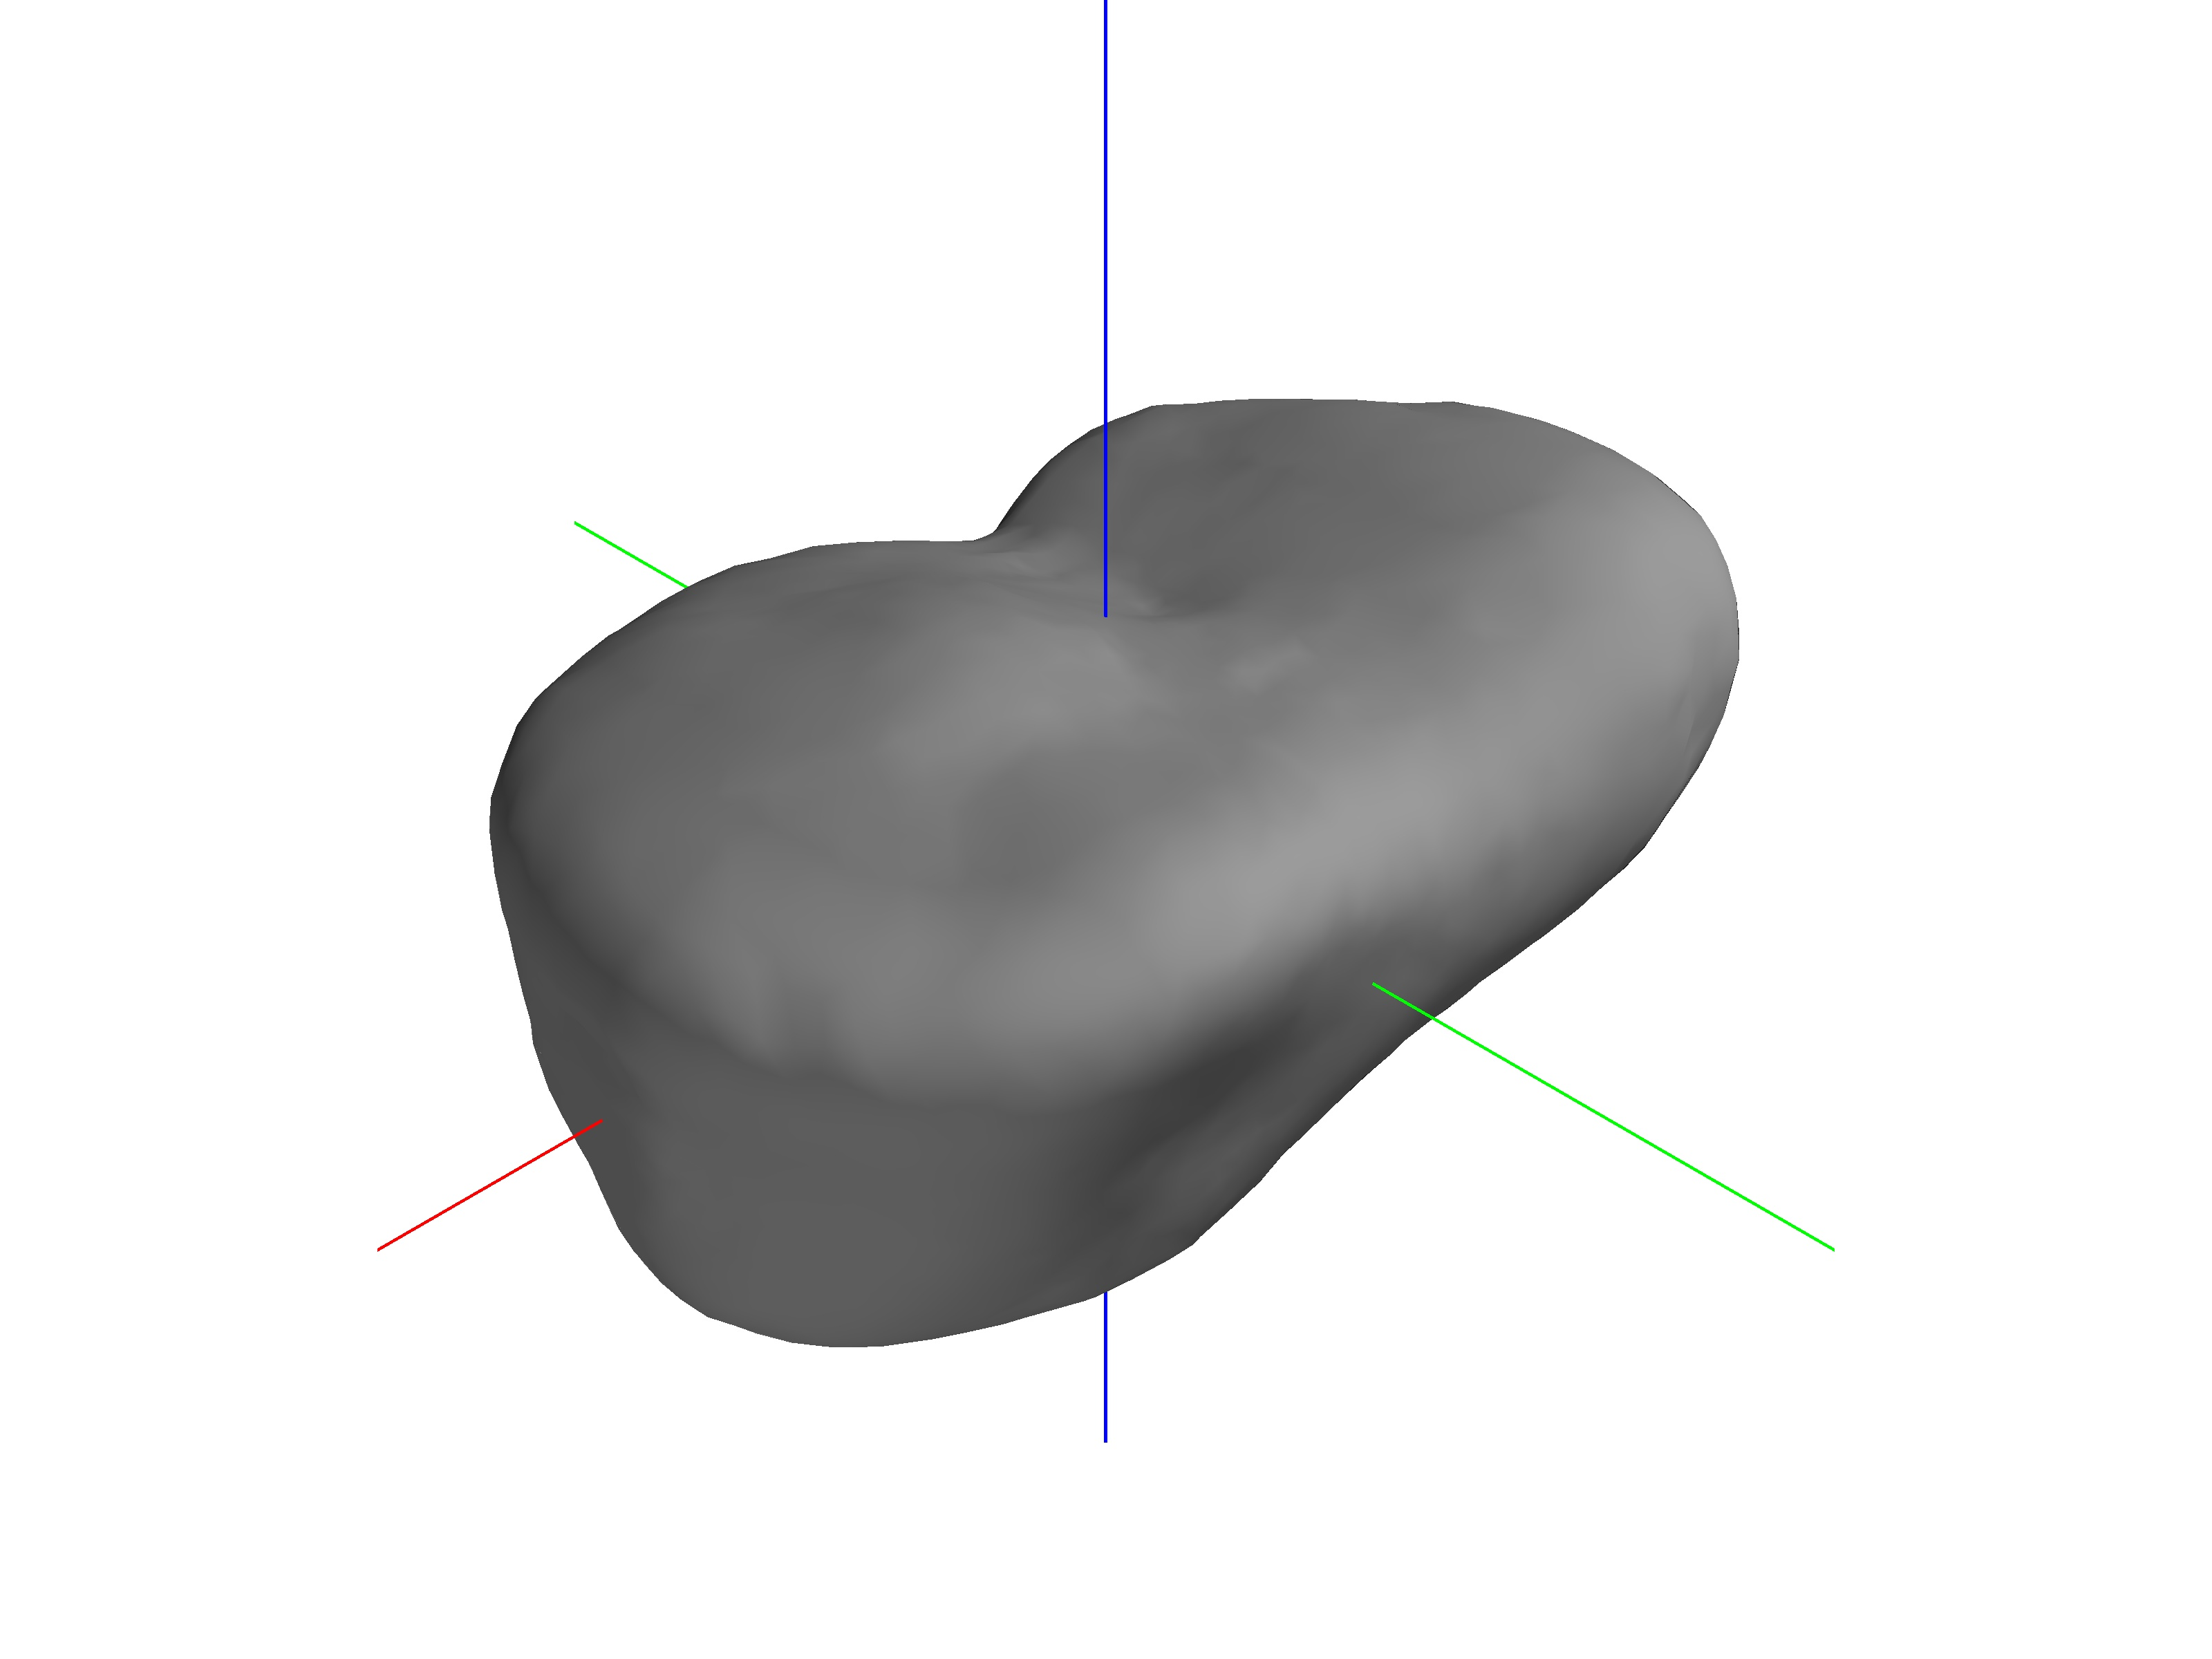
\includegraphics[trim={20cm 10cm 20cm 10cm},clip,keepaspectratio,width=0.5\textwidth,height=\textheight]{figures/dynamic_exploration/castalia/partial_14998.jpg}}
\end{center}

\end{frame}

\begin{frame}{4769 Castalia Refinement}

\begin{center}
    \href{https://youtu.be/pS8vLuRZGxE}{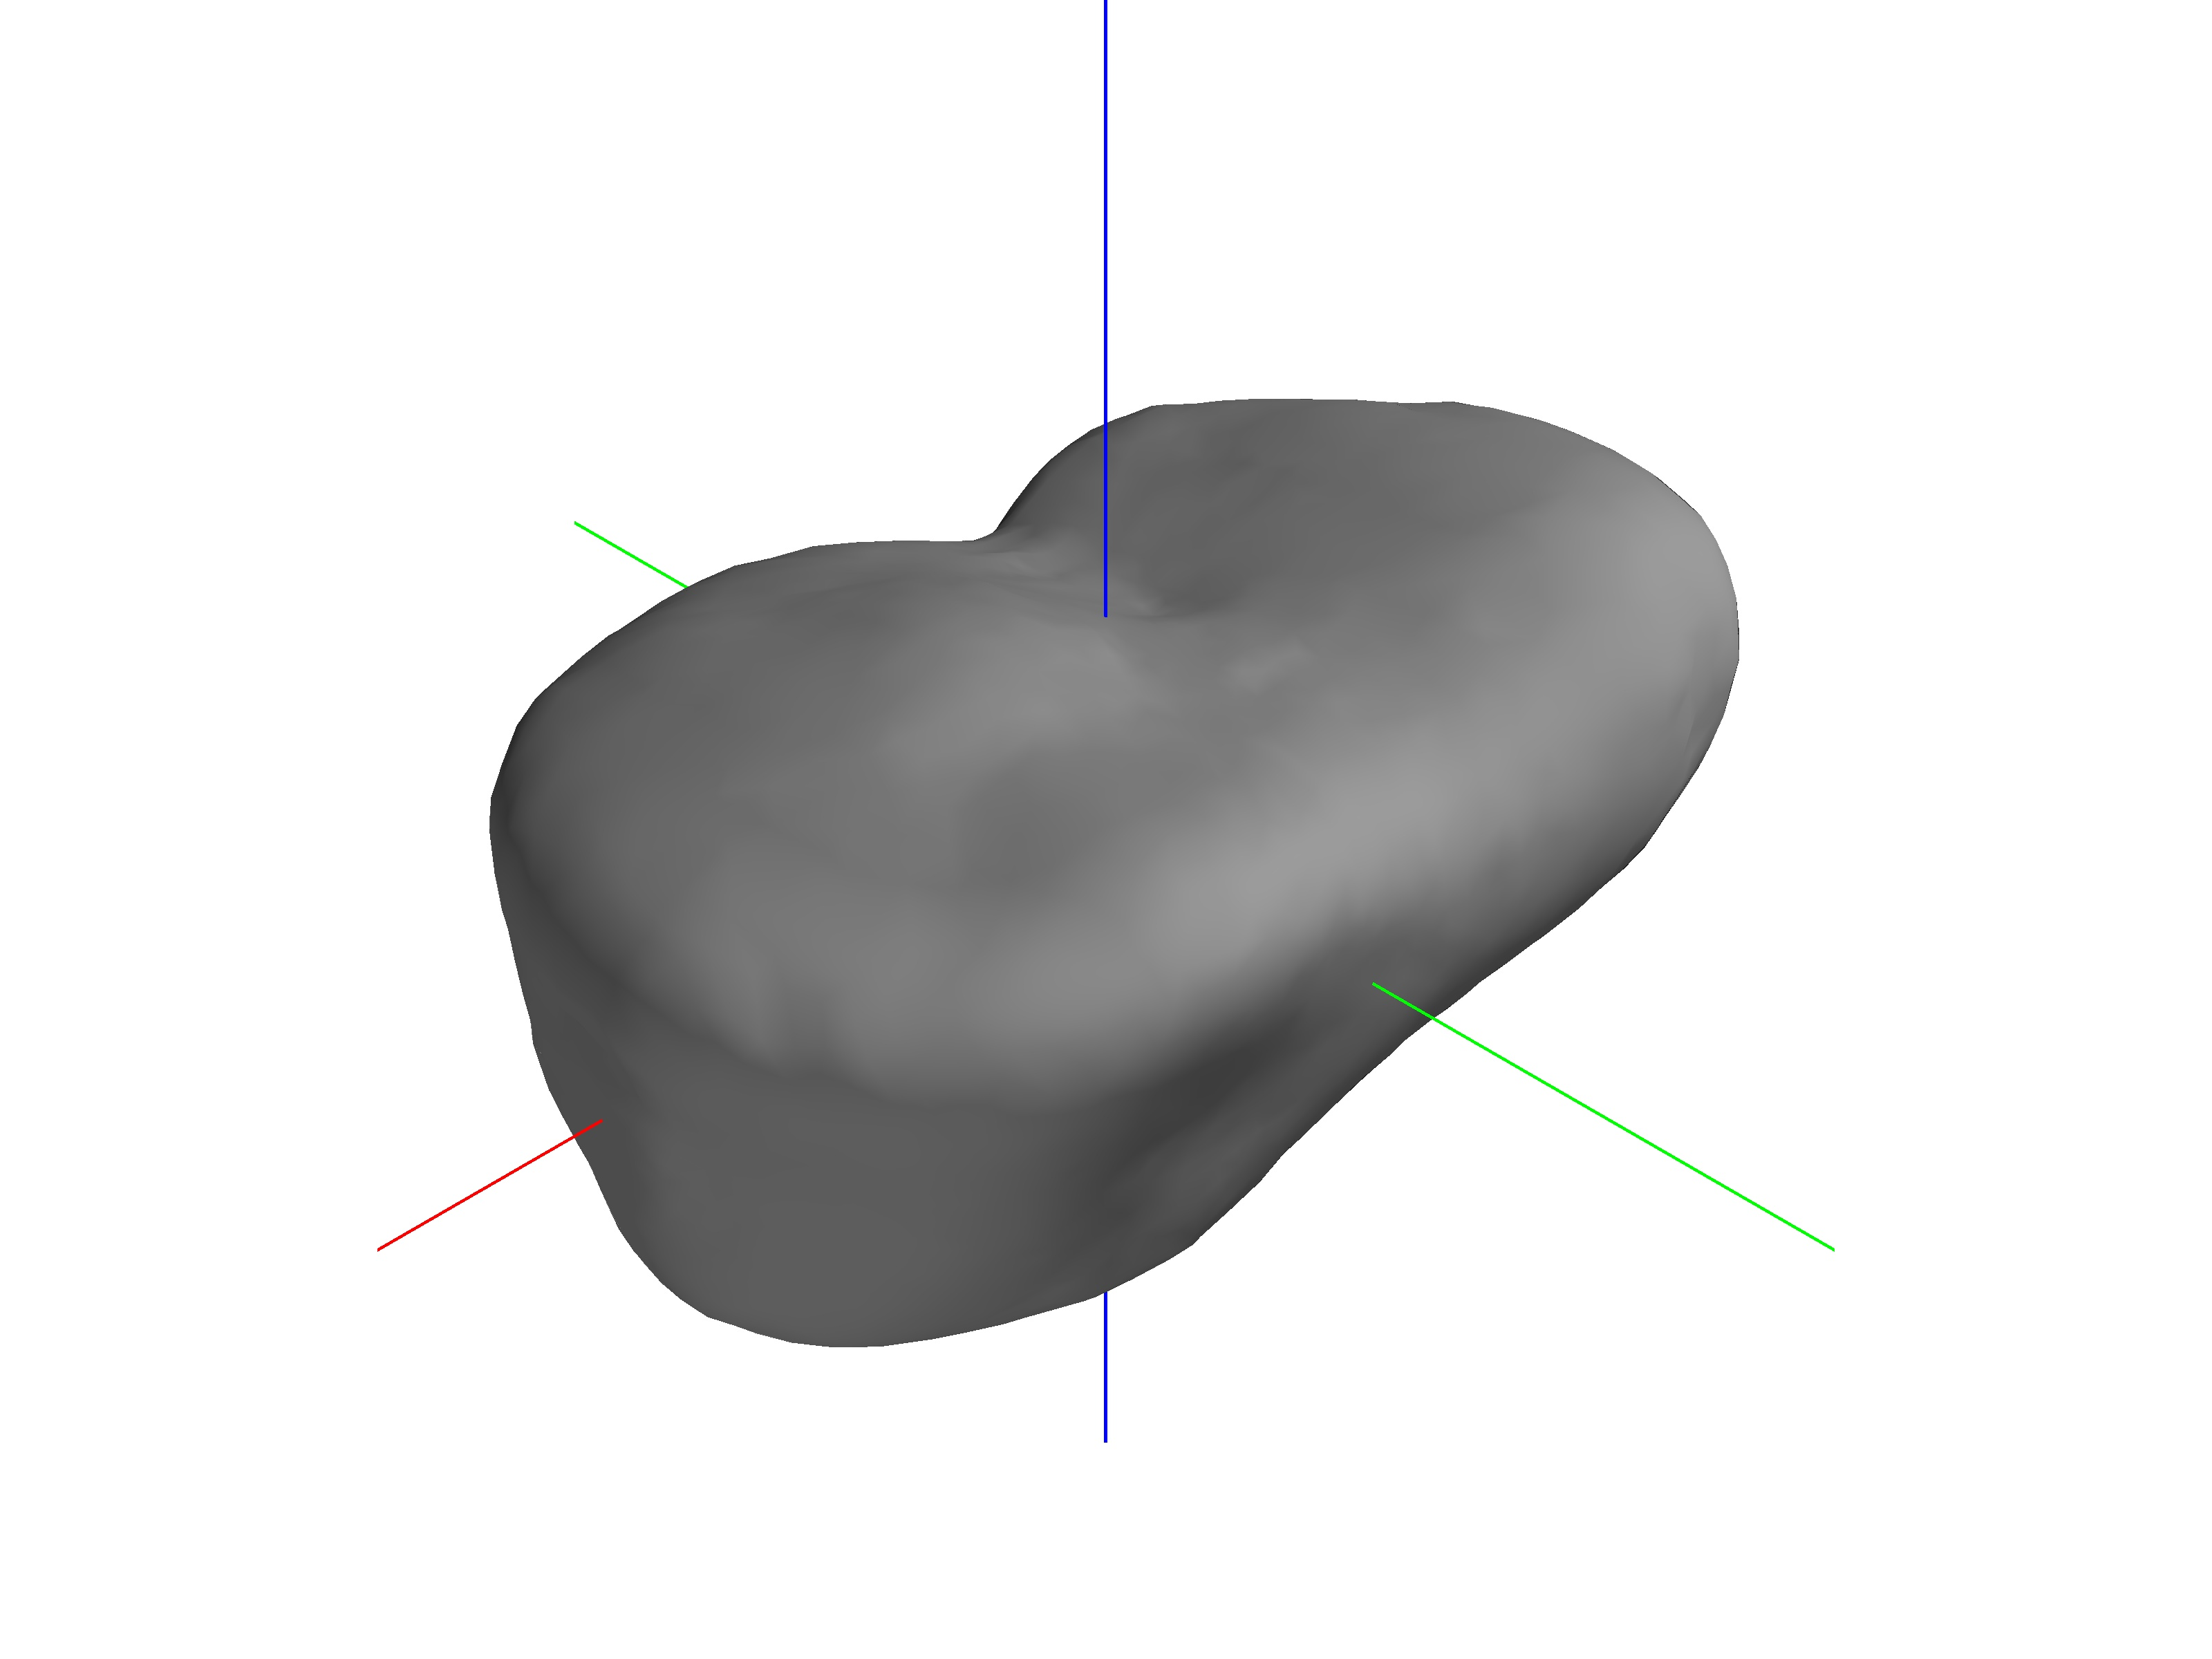
\includegraphics[trim={20cm 10cm 20cm 10cm},clip,keepaspectratio,width=0.5\textwidth,height=\textheight]{figures/dynamic_exploration/castalia/partial_14998.jpg}}%
    \href{https://youtu.be/5ETsFOXQeOs}{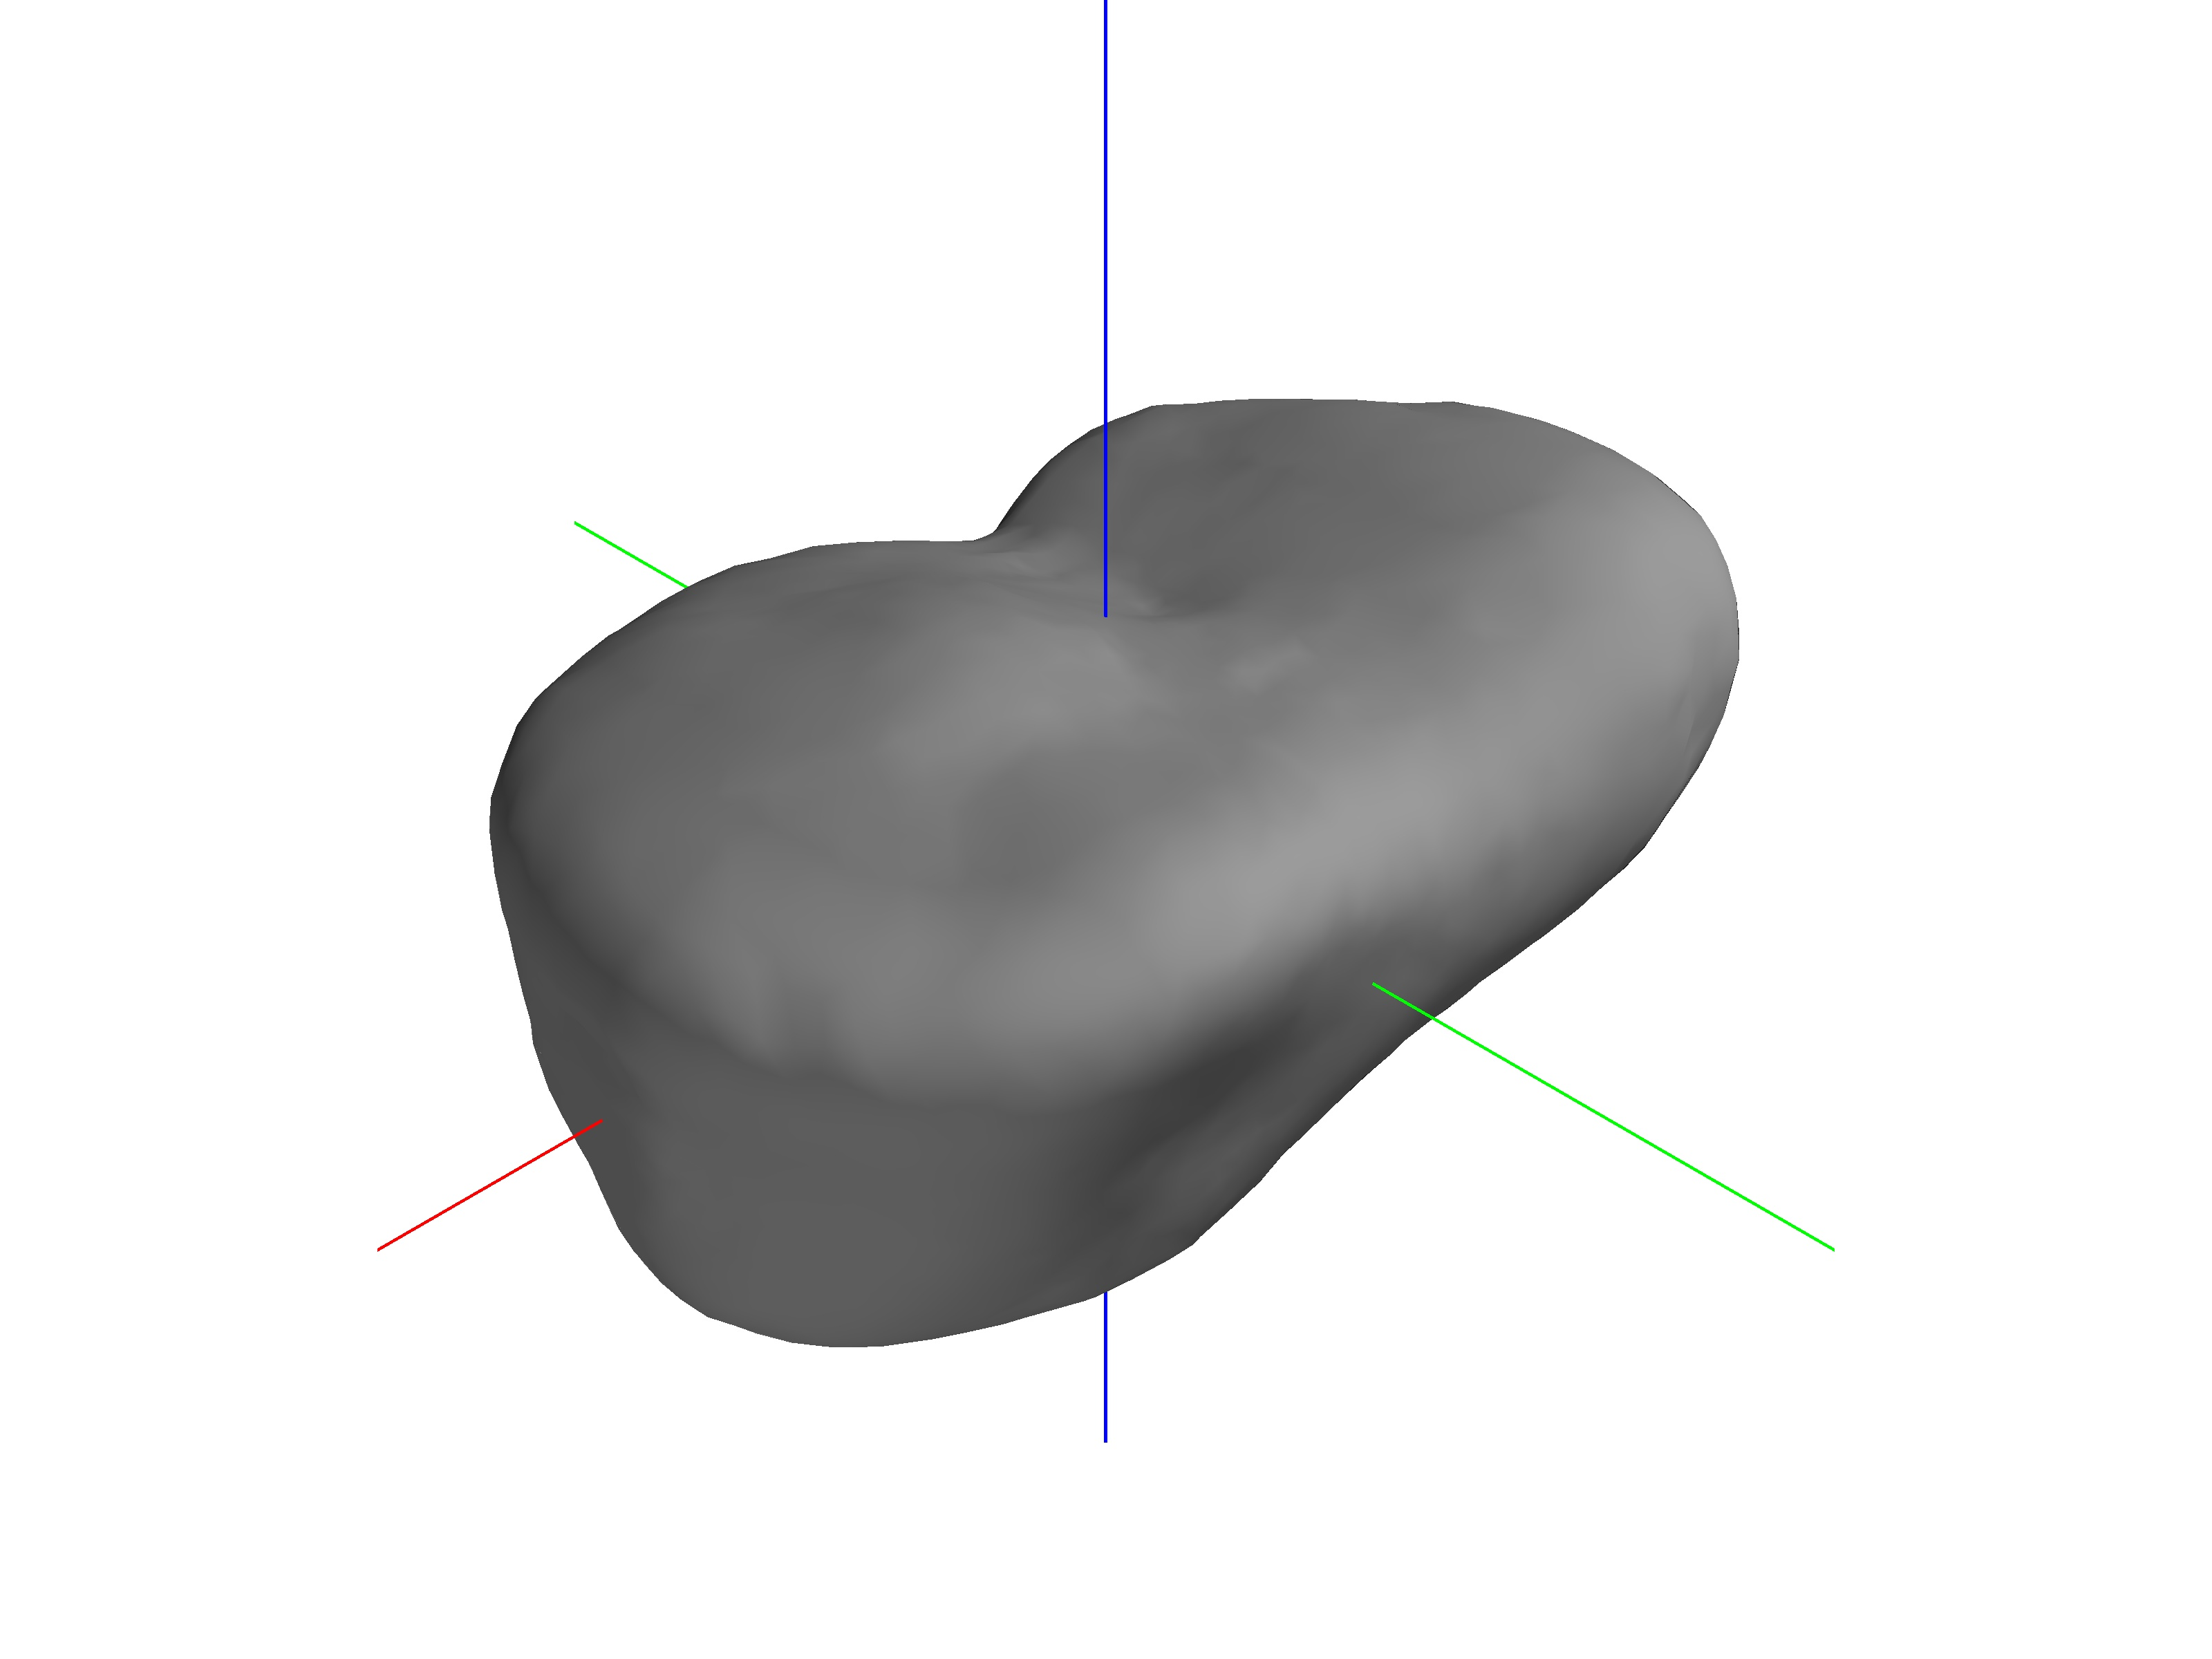
\includegraphics[trim={20cm 10cm 20cm 10cm},clip,keepaspectratio,width=0.5\textwidth,height=\textheight]{figures/dynamic_exploration/castalia/partial_14998.jpg}}
\end{center}

\end{frame}

\begin{frame}{4769 Castalia Landing}

\begin{center}
    \href{https://youtu.be/57sGEJRwfH4}{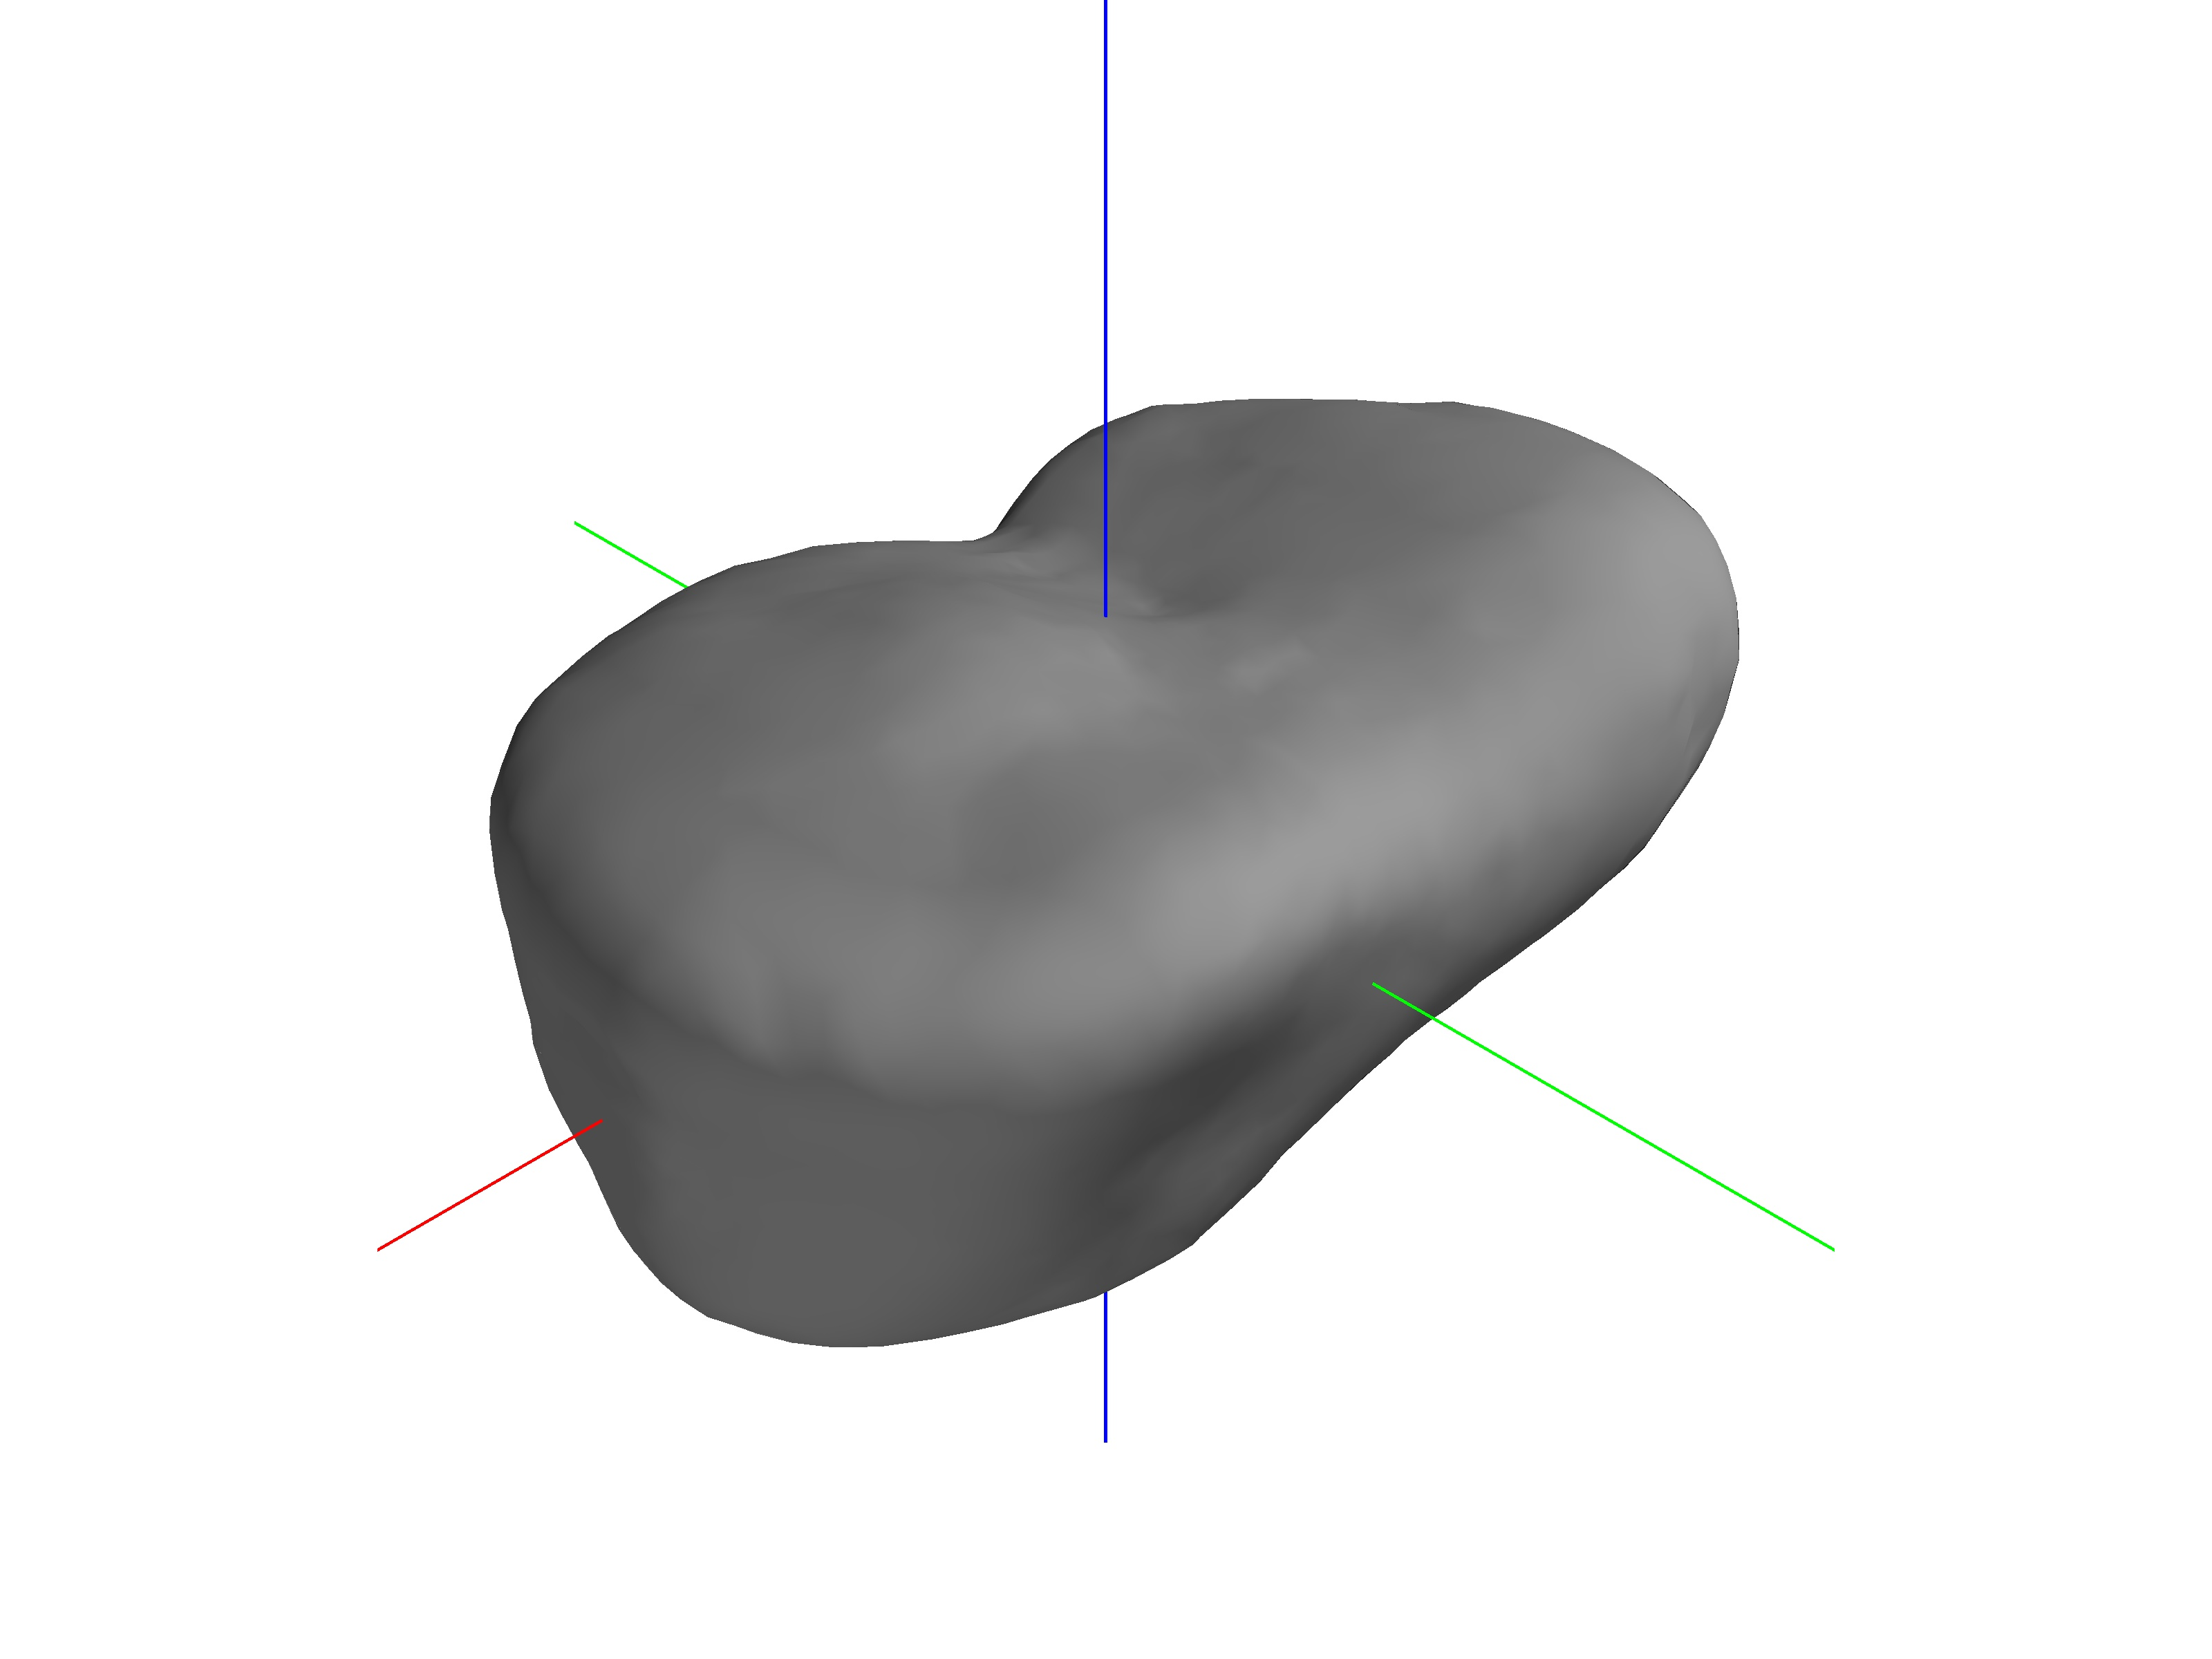
\includegraphics[trim={20cm 10cm 20cm 10cm},clip,keepaspectratio,width=0.5\textwidth,height=\textheight]{figures/dynamic_exploration/castalia/partial_14998.jpg}}%
    \href{https://youtu.be/8igpoKcwqXs}{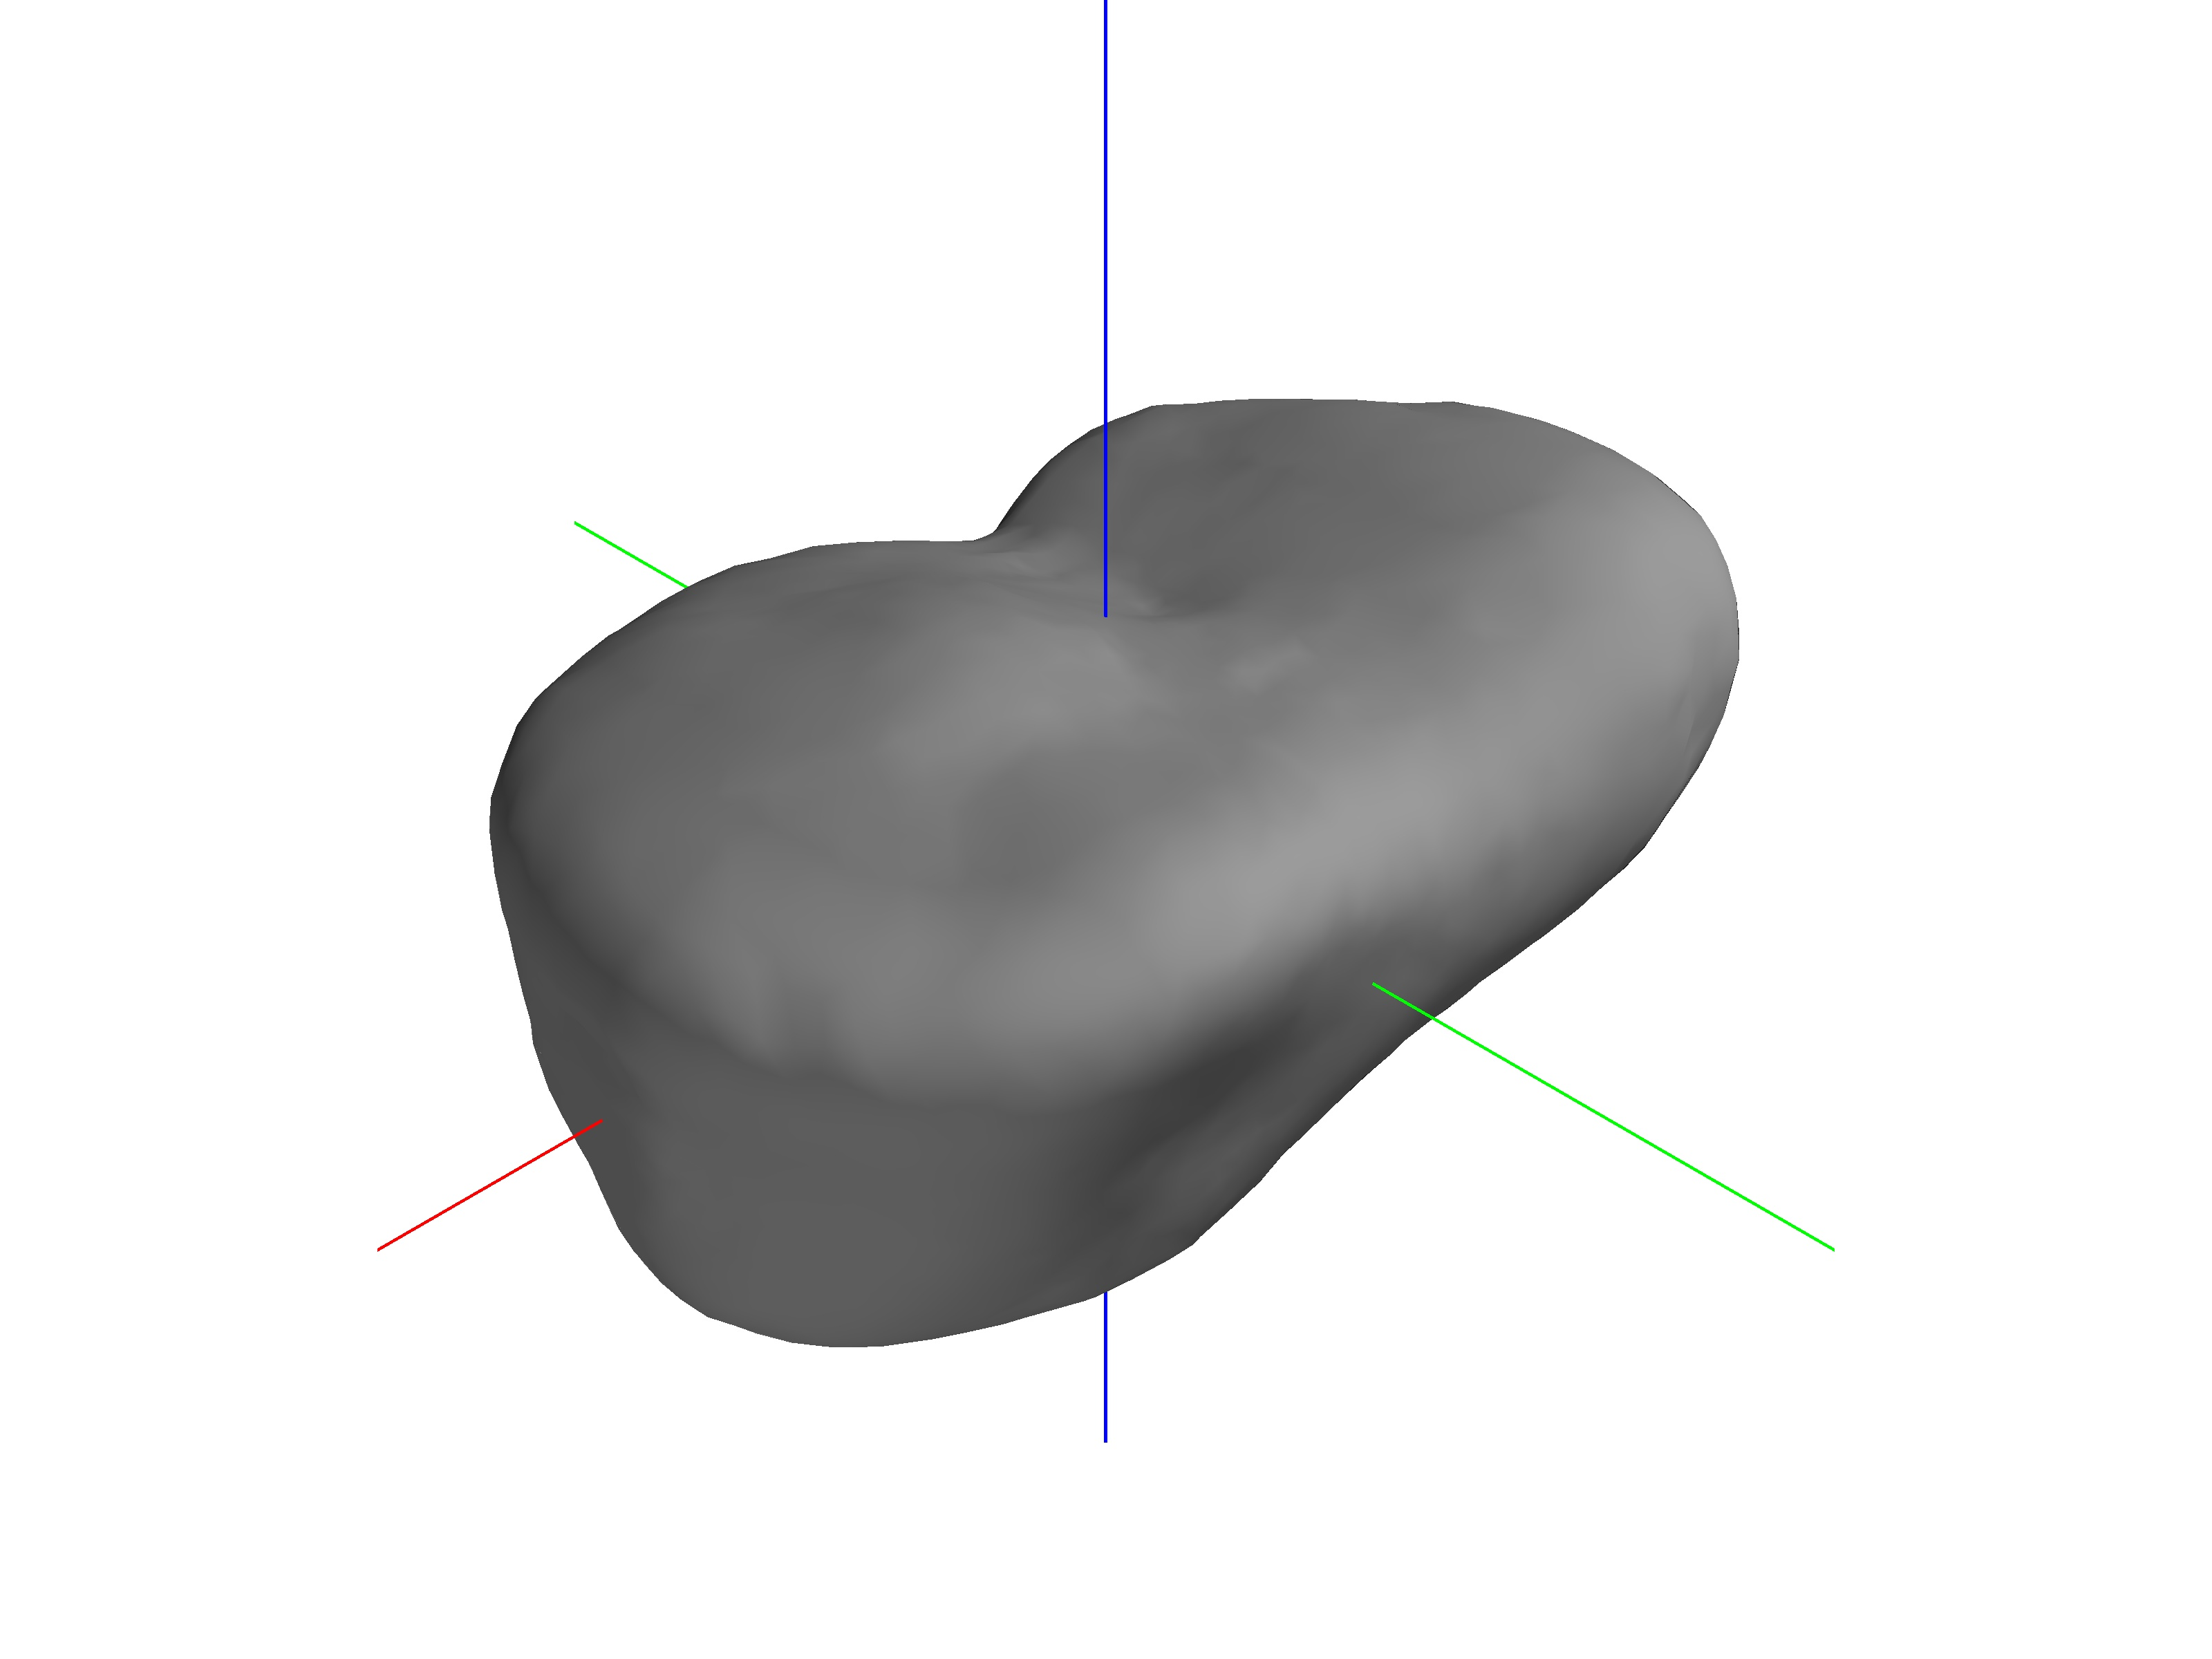
\includegraphics[trim={20cm 10cm 20cm 10cm},clip,keepaspectratio,width=0.5\textwidth,height=\textheight]{figures/dynamic_exploration/castalia/partial_14998.jpg}}
\end{center}

\end{frame}


% !TEX root = ../presentation.tex

\begin{frame}[c]{Thank you}
  \centering
  
  \textbf{\large Flight Dynamics \& Control Lab} \\
  Mechanical \& Aerospace Engineering \\
  School of Engineering \& Applied Science
  
  \begin{center} %figure%
      
\includegraphics[width=0.75\textwidth]{figures/defense/gw_txh_2cs_pos}
    \end{center}
  
  \url{https://fdcl.seas.gwu.edu}
\end{frame}


\end{document}

